% Section of thesis on DUNE 35ton prototype
% Target: 30 pages

\graphicspath{{35ton/Figs/}}

%----------------------------------------------------------------------------------------------------------------------------------------------------------------------------
\chapter{The DUNE 35~ton Prototype}\label{chap:35ton}

The 35~ton is the first experimental prototype of the DUNE far detector design and was briefly introduced in Section~\ref{sec:RoadToDUNE}.  It was originally constructed to demonstrate the unique design features of the LBNE far detector and was the only planned prototype for this experiment.  Following the dissolution of LBNE and the subsequent formation of the DUNE collaboration, the 35~ton has become an integral part of the design and execution of the DUNE far detector design.

As discussed in Section~\ref{sec:LArTPC}, the use of LArTPCs in future long-baseline experiments shows great promise.  To facilitate development of the detector technology, Fermilab has an extensive program of LArTPC experiments culminating in the flagship DUNE project.  Prototying is essential to the success of DUNE as understanding of how to operate progressively larger detectors evolves.  The stategy is staged, with each subsequent phase building on previous success.

The most pertinent issues facing large-scale LArTPCs concern:
\begin{itemize}
  \item the ability to achieve and maintain the necessary LAr purity for successful data taking;
  \item the design and construction of huge underground cryostats.
\end{itemize}
The research and development performed thus far have demonstrated viable solutions to these obstacles and has resulted in the situation where ProtoDUNE can be attempted with confidence.

The outcomes of each of these projects at Fermilab are the subject of this present chapter.  The first of the above issues, regarding LAr purity, is discussed in Section~\ref{sec:MTSLAPD} with reference to the Materials Test Stand and the Liquid Argon Purity Demonstrator.  The second complication, concerning the construction of large underground cryostats, was the main motivation for the 35~ton Phase~I experiment and is the subject of Section~\ref{sec:35tonPhaseI}.  The culmination of all these developments involved operating a small scale LArTPC alongside these improvements and was achieved in the 35~ton Phase~II run, discussed in Section~\ref{sec:35tonPhaseII}.  Since this experiment forms the basis for later chapters, it will be reviewed in much greater detail.  A summary of all this R\&D is presented in Section~\ref{sec:35tonSummary}.

%----------------------------------------------------------------------------------------------------------------------------------------------------------------------------
\section[The Materials Test Stand and Liquid Argon Purity Demonstrator]{The Materials Test Stand and\\Liquid Argon Purity Demonstrator}\label{sec:MTSLAPD}

Work developing LArTPCs for future neutrino experiments began at FNAL in 2007 with a view to eventually facilitating a multi-kton LAr experiment.  Even utilising a modular design, as with the DUNE far detector (Section~\ref{sec:FarDetector}), drift distances on the order of a few metres are realistically required, necessitating a low concentration of electronegative impurities.  Attaining and holding the requisite LAr purity in a huge underground cryostat over many years of running is a considerable challenge addressed by the test stands reviewed in this section.

%----------------------------------------------------------------------------------------------------------------------------------------------------------------------------
\subsection{The Materials Test Stand}\label{sec:MTS}

The Materials Test Stand (MTS) \cite{MTS2006,MTS2009a,MTS2009b,MTS2011} was constructed at FNAL to develop LAr purification techniques and to characterise the effect of various materials on the electron lifetime when submerged in the liquid.  It consists of a small cryostat and two filters containing activated-copper-coated granules and an adsorbent molecular sieve respectively; a schematic of the MTS setup is shown in Figure~\ref{fig:MTS}.  The filters are designed to remove oxygen and water contaminants with functionality similar to that successfully demonstrated by the ICARUS collaboration \cite{ICARUS1993b}.  Oxygen is removed by the copper beads using the chemical reaction
\begin{equation}
  2~\textnormal{Cu} + \textnormal{O}_2 \rightarrow 2~\textnormal{CuO}
\end{equation}
and water molecules are physically trapped in the microporous structure of the sieve.  The filters additionally contain the ability to be regenerated in situ, a necessity when planning a long-running experiment, multi-kton experiment; those used previously were primarily proprietary \cite{ICARUS1993a,ICARUS2006}.

\begin{figure}
  \centering
  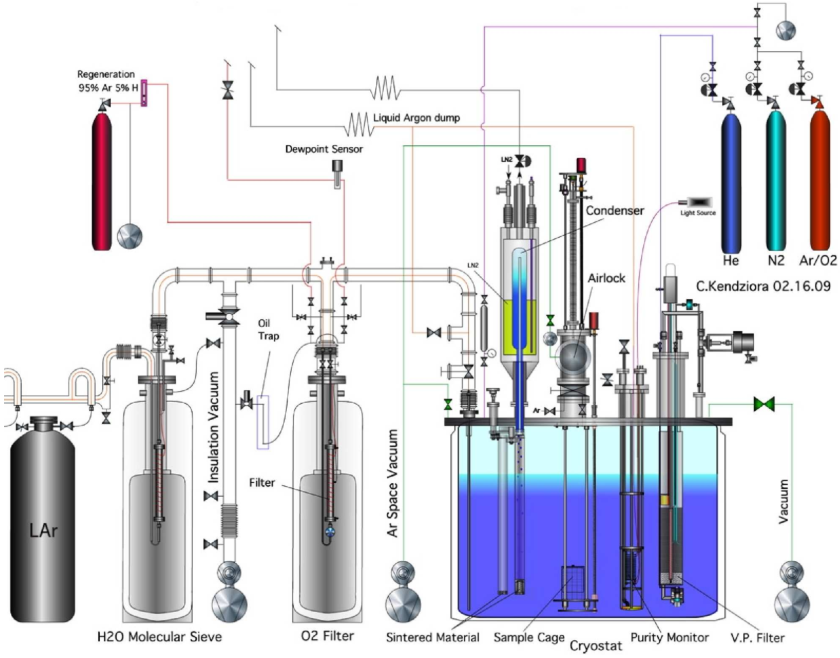
\includegraphics[width=14cm]{MTS.pdf}
  \caption[The Materials Test Stand Stand at FNAL.]{The Materials Test Stand Stand at FNAL \cite{MTS2009b}.  Liquid argon used to fill the cryostat flows from left to right in the schematic, through two filters designed to reduce the H$_2$O and O$_2$ contamination respectively.  A second filter system (the `vapour pump' (V.P.)), using the same materials, is installed within the cryostat to remove impurities introduced by the materials being examined.}
  \label{fig:MTS}
\end{figure}

The MTS successfully demonstrated good argon purity ($<3$~ppb~H$_2$O) and showed the primary opposition to electron lifetime is water contamination, demonstrated in Figure~\ref{fig:MTSResults}.  It was found that exposure to warm surfaces in the cryostat, such as above the liquid level, facilitated contamination from water impurities as they remain on surfaces even in a vacuum.  The condenser used in the MTS to recondense gaseous argon returned it directly to the liquid in the cryostat (as `raining' condensation) and was found to dramatically reduce the LAr purity when in use.  This is due to contaminants introduced into the gas by exposure to the warm croystat walls which could be negated by returning the liquid via a different path which maximised subjection to cold surfaces.  Notably, the electron lifetime was found to be unaffected on the introduction of test materials, although as suspected the temperature of the materials did have an impact.  This is a hugely promising result for the future of LArTPC design and construction.

\begin{figure}
  \centering
  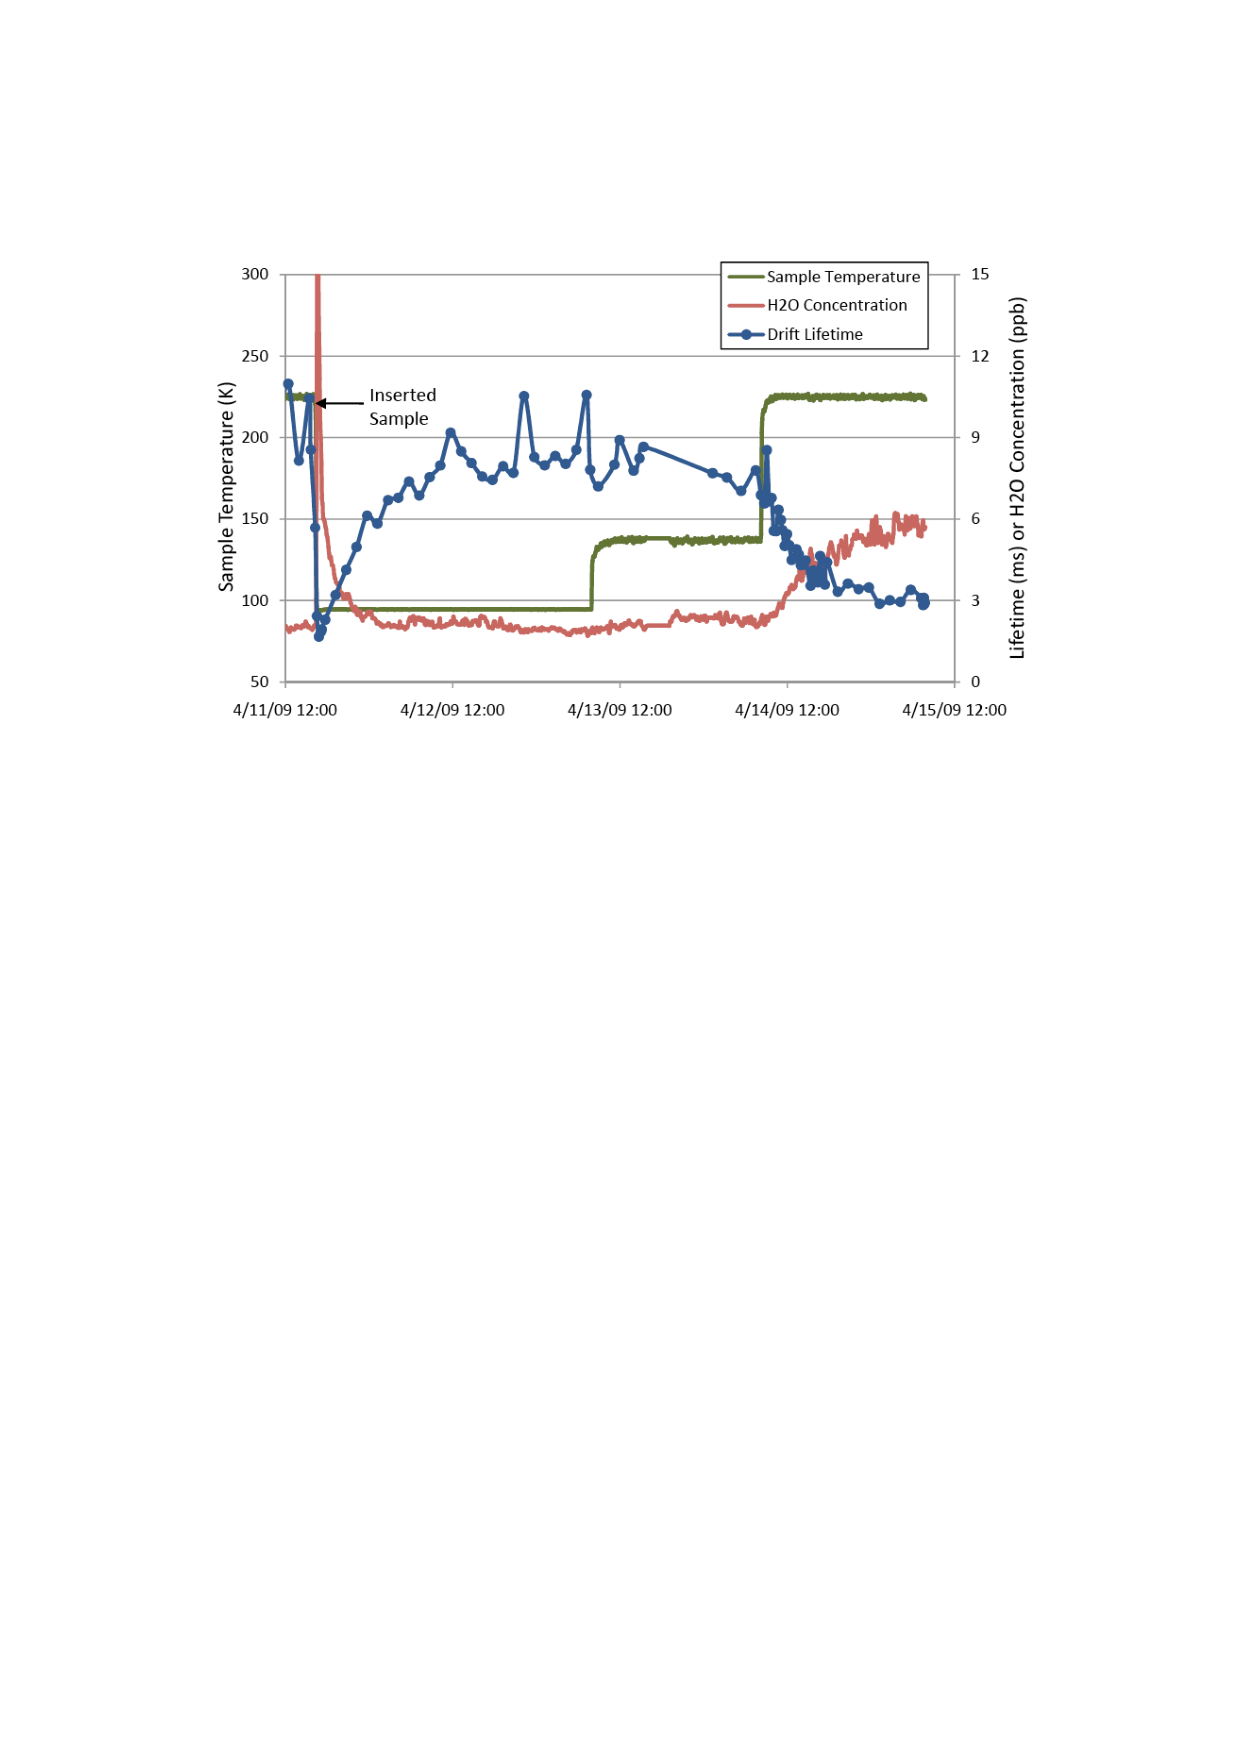
\includegraphics[width=12cm]{MTSResults.pdf}
  \caption[Results from the Materials Test Stand showing the water contamination in LAr and the corresponding electron lifetime.]{Results from the Materials Test Stand showing the water contamination in LAr and the corresponding electron lifetime \cite{MTS2009a}.  There is an obvious inverse correlation between the density of electronegative (H$_2$O) impurities and the resulting lifetime.}
  \label{fig:MTSResults}
\end{figure}

%----------------------------------------------------------------------------------------------------------------------------------------------------------------------------
\subsubsection{Filter Regeneration}\label{sec:FilterRegeneration}

Over time, the filters become less effective as electronegative impurities accumulate.  A significant success of the MTS was demonstrating the process of regenerating the filters in situ.  This is achieved by heating the vessels to 250$^{\circ}$C and, in the case of the molecular sieve, simply using a vacuum pump to remove the water vapour or, in the case of the activated copper, by pumping through a 95:5 mixture of Ar:H$_2$ gas to capture the oxygen through the reduction reaction
\begin{equation}
  \textnormal{CuO} + \textnormal{H}_2 \rightarrow \textnormal{Cu} + \textnormal{H}_2\textnormal{O}.
\end{equation}
During the running of the test stand, the filters were regenerated after the passage of around 1000~litres of liquid argon.

%----------------------------------------------------------------------------------------------------------------------------------------------------------------------------
\subsubsection{Purity Monitoring}\label{sec:PurityMonitoring}

The ability to constantly evaluate the LAr purity during an experimental run is hugely important to ensure high quality data.  The impurity concentrations are typically beyond the capabilities of many conventional gas analysers and so a custom device, known as a `purity monitor' (PrM), is utilised.  The design is based on the purity monitors developed by ICARUS \cite{ICARUSPurityMonitor} and is shown in Figure~\ref{fig:PurityMonitor}.

\begin{figure}
  \centering
  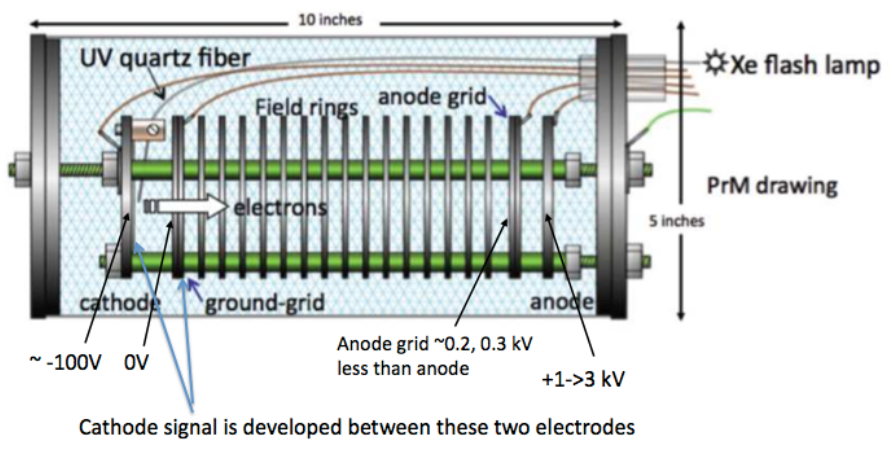
\includegraphics[width=10cm]{PurityMonitor.png}
  \caption[Schematic design of the purity monitors utilised at the FNAL LAr test stands.]{Schematic design of the purity monitors utilised at the FNAL LAr test stands \cite{}.  Purity monitors using this design were pioneered by ICARUS \cite{ICARUSPurityMonitor} and used in the MTS along with the subsequent Liquid Argon Purity Demonstrator (Section~\ref{sec:LAPD}) and 35~ton Runs I (Section~\ref{sec:35tonPhaseI}) and II (Section~\ref{sec:35tonPhaseII}).}
  \label{fig:PurityMonitor}
\end{figure}

The PrM consists of a cylindrical volume containing LAr from its surrounding environment and an anode and photocathode separated by a short drift region.  When taking purity measurments, light from a Xenon flash lamp is incident on the cathode, liberating photoelectrons which traverse towards the anode.  Electronegative impurities in the LAr will decrease the electron lifetime and therefore the number of electrons reaching a certain point along the drift volume.  A measurement of the ratio of the charge arriving at the anode to that at the cathode is hence a measurement of the inherit purity of the liquid.

The MTS cryostat contains a purity monitor and they were subsequently used in the Liquid Argon Purity Demonstrator and the 35~ton.  When developed for the Liquid Argon Purity Demonstrator and 35~ton cryostats, two sizes were used; long (47~cm) and short (16~cm).

%----------------------------------------------------------------------------------------------------------------------------------------------------------------------------
\subsection{The Liquid Argon Purity Demonstrator}\label{sec:LAPD}

The Liquid Argon Purity Demonstrator (LAPD) \cite{MTS2011,LAPD2014,LAPDJINST2014} was designed to demonstrate the required purity of LArTPC experiments is possible without the use of large scale vacuum pumps.  Previous and current LArTPC experiments, such as ICARUS, Argoneut, LArIAT and MicroBooNE, have been constructed as flat plane vessels and have used an evacuation method as the first step in removing atmospheric impurities to facilitate the required LAr purity.  The necessary mechanical capability of the cryostat to withstand this process, along with the associated equipment, results in unfeasible engineering challenges and costs as detectors increase to multi-kton scales.

In order to circumvent these issues, a design utilising multiple smaller-scale cryostats was proposed.  This however leads to greater complexity relating to both the engineering requirements of the piping infrastructure and the reconstruction capabilities of interactions spanning multiple active volumes.  LAPD successfully pioneering an alternative approach, using a `piston purge' as a first purification step to remove atmospheric impurities.  This is a hugely important result and has significantly influenced the design of future LArTPC experiments, including the 35~ton.  Additionally, although designed to be evacuated with vacuum pumps, MicroBooNE was filled using the piston purge technique following the success of LAPD.

%----------------------------------------------------------------------------------------------------------------------------------------------------------------------------
\subsubsection{LAPD Experimental Setup}\label{sec:LAPDExperimentalSetup}

The LAPD cryostat is shown in Figure~\ref{fig:LAPD}.  It consists of a cylindrical tank, diameter 10~feet and height 10~feet, with a domed head capable of holding 32.6~ton LAr.  It is physically next to the MTS and uses the purification system prototyped by this previous effort.  Insulation for the tank is provided by fibreglass sheets covering the outer volume which, along with the tank, is refrigerated by liquid nitrogen (LN$_2$) from an external supply.  As with the MTS, a condenser is utilised above the croystat to recondense argon gas using coils also cooled with LN$_2$.  This liquid is subsequently sent through the filtration system before being returned to the main volume, a consequense of the previous R\&D with the MTS.  After filling, the system is closed and a good LAr purity is maintained by constant circulation of the cryostat content through the filters.

The system is instrumented with PrMs, gas analysers and temperature sensors.  Four PrMs are contained within the cryostat to measure the purity gradient with an additional one just after the filters to sample to liquid before it is returned to the main volume.  Along with purity, the temperature gradient is measured in order to study the effect of this on electron drift velocity.  The contaminants in the LAr are quantified using nitrogen, oxygen and water analysers outside of the main volume.

\begin{figure}
  \centering
  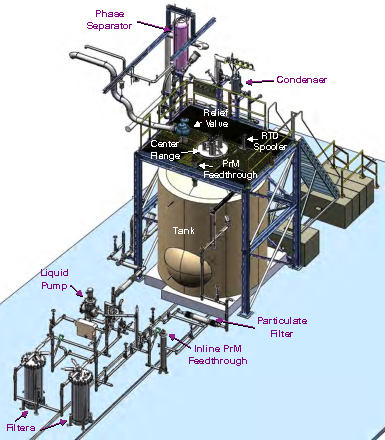
\includegraphics[width=10cm]{LAPD.pdf}
  \caption[The Liquid Argon Purity Demonstrator cryostat and purification system.]{The Liquid Argon Purity Demonstrator cryostat and purification system \cite{LAPDJINST2014}.The two cylinders at the bottom left are the filters described in Section~\ref{sec:MTS}.  The piping facilitates the transport of LAr into and out of the cryostat so continual purification within a closed system may be achieved.}
  \label{fig:LAPD}
\end{figure}

%----------------------------------------------------------------------------------------------------------------------------------------------------------------------------
\subsubsection{Filling LAPD}\label{sec:FillingLAPD}

The piston purge technique involves injecting warm argon gas at high pressure at the bottom of the cryostat with the top open for venting, demonstrated in Figure~\ref{fig:LAPDPistonPurgeSchematic}.  The heavier than air argon gas acts as a piston, forcing the ambient air out of the top of the cryostat.  Figure~\ref{fig:LAPDPistonPurgeImpurities} demonstrates how this successfully reduces the impurity concentration in the cryostat, shown as a function of complete volume changes.  After completion of the piston purging, the O$_2$ contamination had decreased from 21\% to 6~ppm, N$_2$ from 78\% to 18~ppm and H$_2$O from 200~ppm to 1.2~ppm.

\newsavebox{\largestimage}

\begin{figure}
  \centering
  %\savebox{\largestimage}{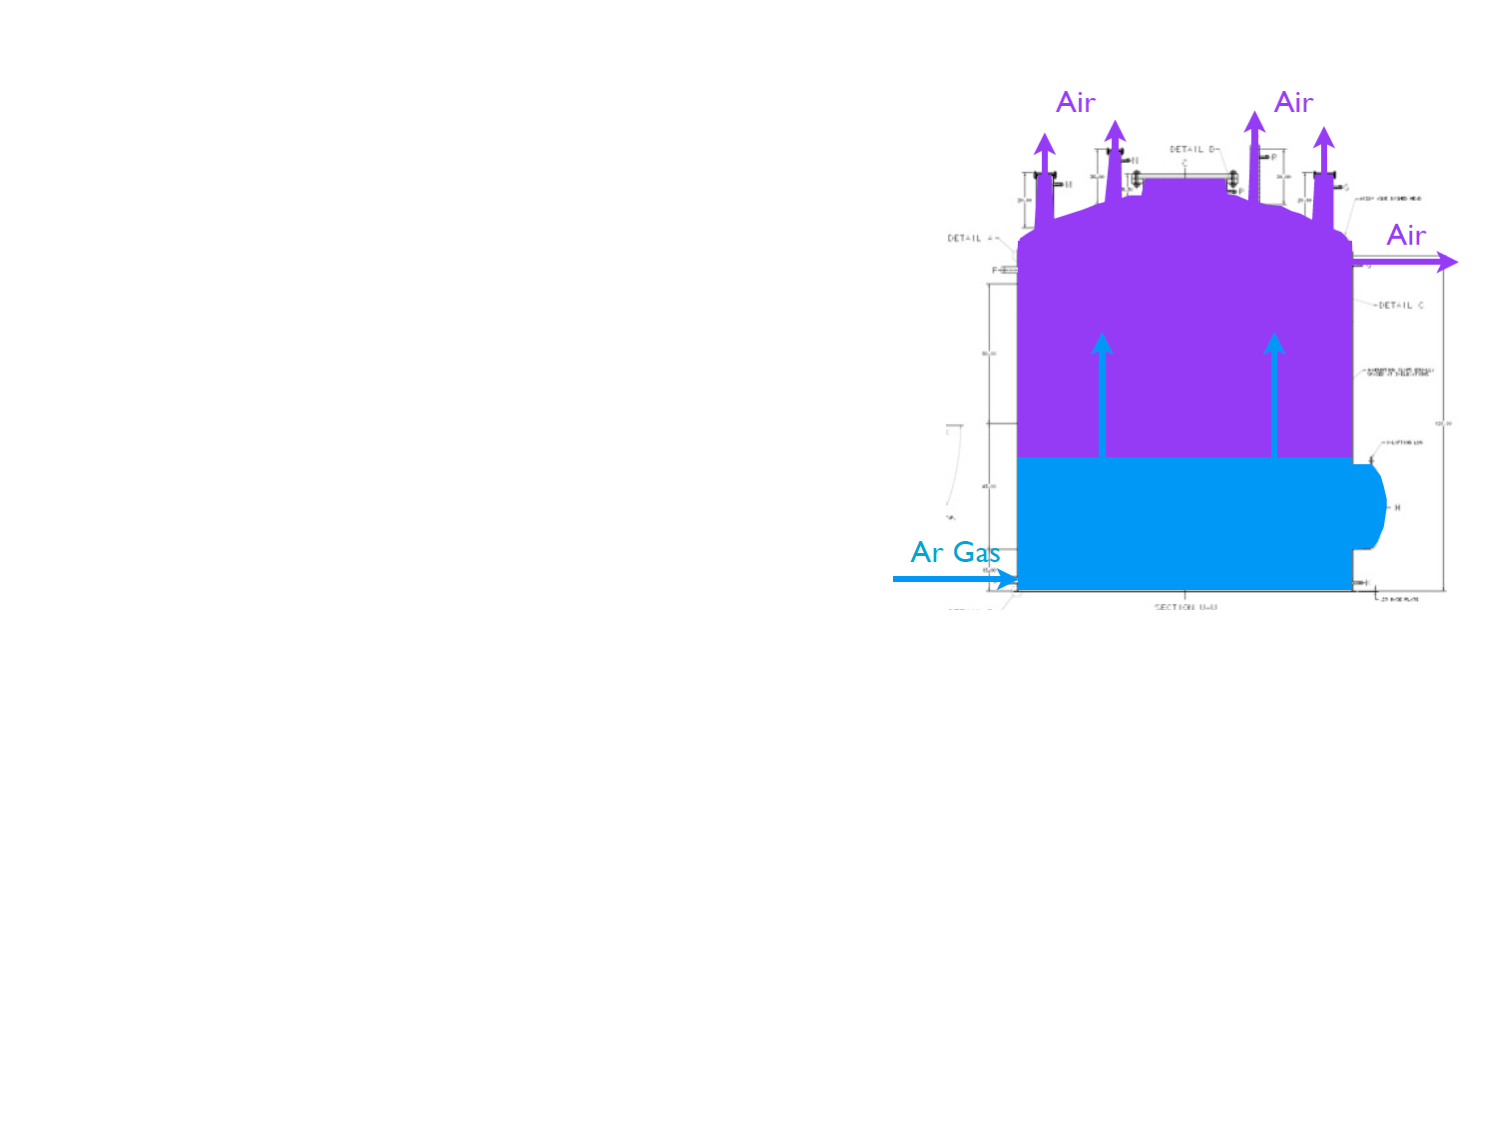
\includegraphics[width=0.49\textwidth]{LAPDPistonPurgeSchematic.pdf}}
  \begin{subfigure}[t]{0.5\linewidth}
    \centering
    %\usebox{\largestimage}
    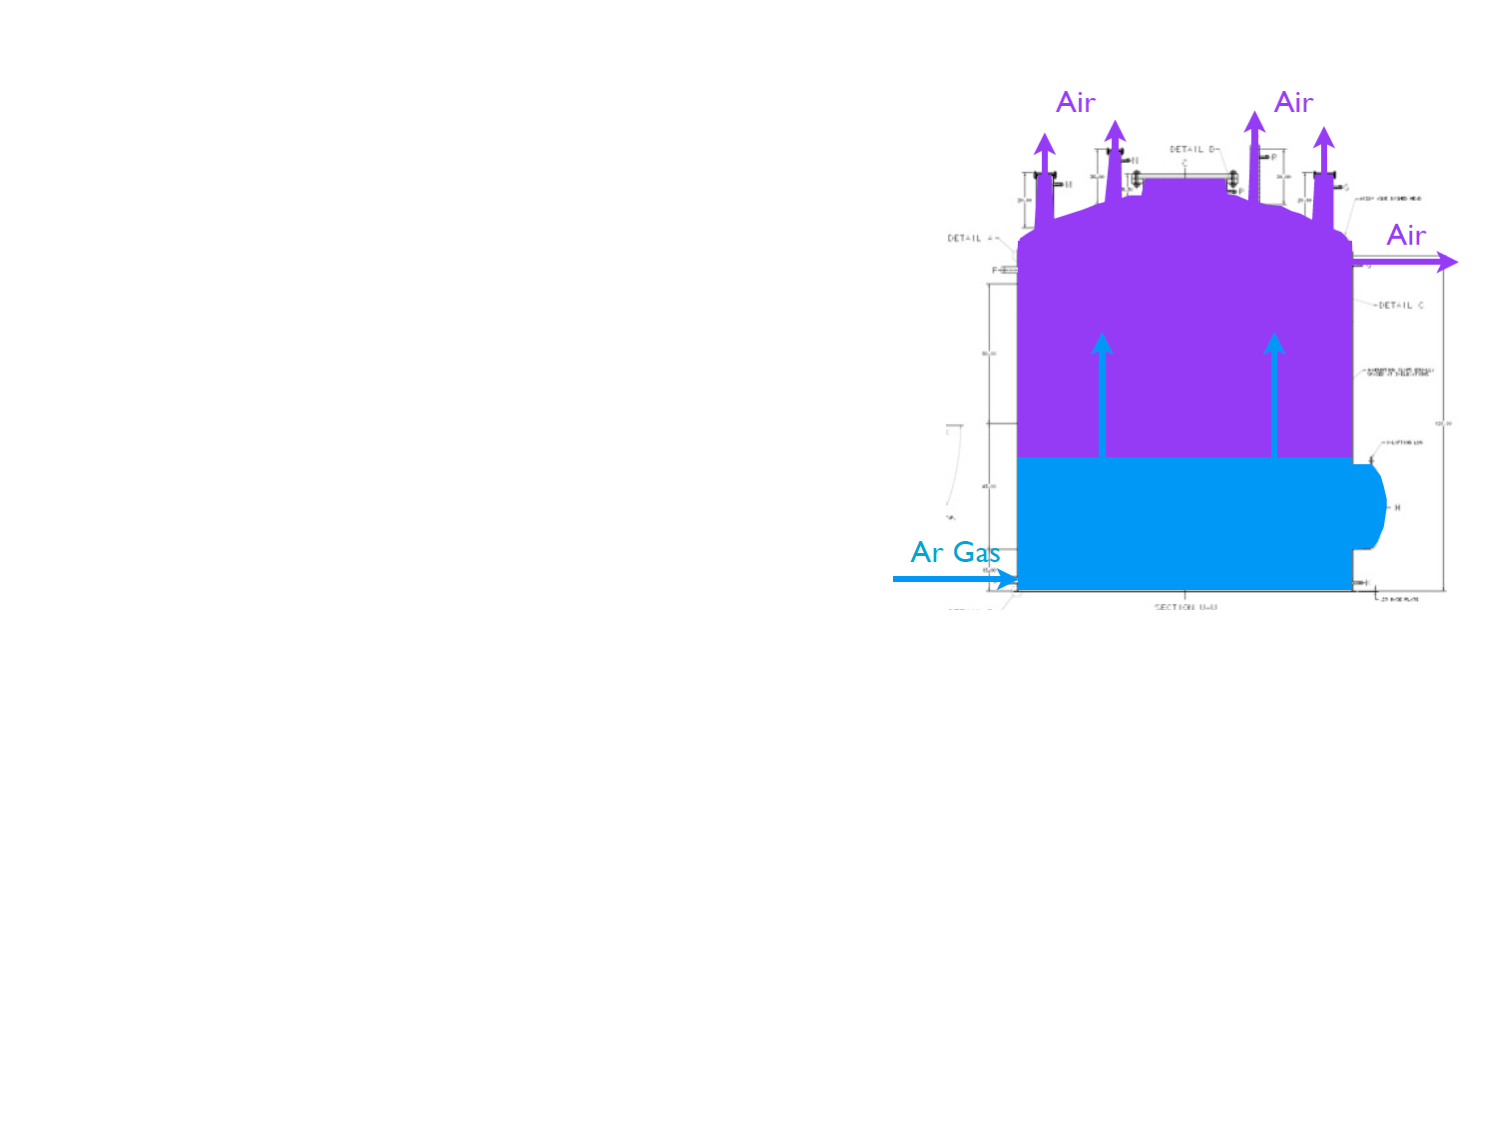
\includegraphics[width=0.98\textwidth]{LAPDPistonPurgeSchematic.pdf}
    \caption{Schematic of the LAPD piston purge.}
    \label{fig:LAPDPistonPurgeSchematic}
  \end{subfigure}\vspace{5mm}
  \begin{subfigure}[t]{0.7\linewidth}
    \centering
    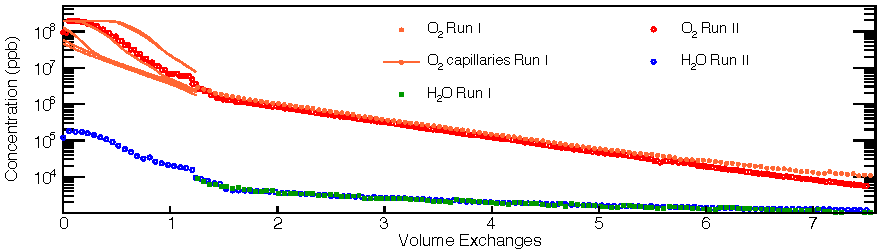
\includegraphics[width=0.98\textwidth]{LAPDPistonPurgeImpurities.pdf}
    %\raisebox{\dimexpr.5\ht\largestimage-.5\height}{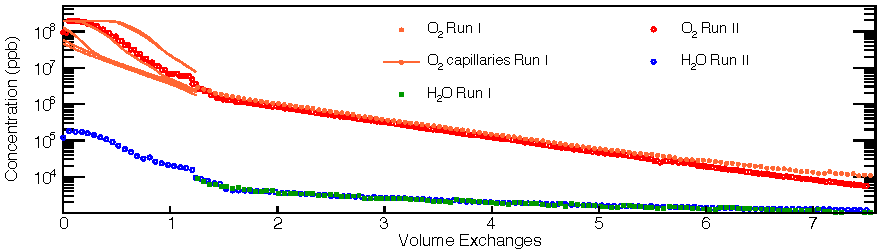
\includegraphics[width=\textwidth]{LAPDPistonPurgeImpurities.pdf}}
    \caption{LAPD impurity concentration during the piston purge.}
    \label{fig:LAPDPistonPurgeImpurities}
  \end{subfigure}
  \caption[The piston purge technique in the Liquid Argon Purity Demonstrator to remove atmopheric impurities before filling.]{The piston purge technique in the Liquid Argon Purity Demonstrator to remove atmopheric impurities before filling \cite{LAPDJINST2014}.  The results from two LAPD runs are shown, the first with the cryostat only half filled to prototype the technique.  Discontinuities between the impurity concentrations are caused by switches between gas analysers.}
  \label{fig:LAPDPistonPurge}
\end{figure}

Following the filling of the cryostat with gaseous argon, the contents are then continually circulated through the filters to further reduce the impurities present.  The improved electronegative concentrations are shown, again with reference to the number of complete volume changes, in Figure~\ref{fig:LAPDGasCirculation}.  This lasted, as can also be observed in the figure, for a number of days and resulted in a much improved O$_2$ contamination of around 20~ppb and an H$_2$O level which balanced the outgassing rate from the warm cryostat surfaces.

\begin{figure}
  \centering
  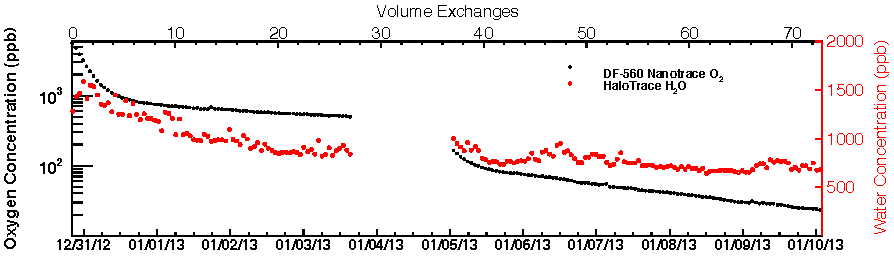
\includegraphics[width=0.7\linewidth]{LAPDGasCirculation.pdf}
  \caption[The concentration of electronegative impurities during the gas circulation stage in the Liquid Argon Purity Demonstrator following the piston purge.]{The concentration of electronegative impurities during the gas circulation stage in the Liquid Argon Purity Demonstrator following the piston purge \cite{LAPDJINST2014}.  The stabilisation of the oxygen contamination signified a leak, which was fixed during the break in readings.}
  \label{fig:LAPDGasCirculation}
\end{figure}

The filling can thus proceed by transporting LAr into the cryostat through the filter system, to ensure a high purity in maintained.  The impurity concetrations were inspected before filling and after filtration and in total, a volume of 29.7~ton LAr was supplied to the LAPD cryostat.  Once filled, and during the course of operations, the liquid argon volume was constantly recirculated through the filtration system to preserve the LAr purity.  This is shown schematically in Figure~\ref{fig:LAPDLiquidCirculation}.

\begin{figure}
  \centering
  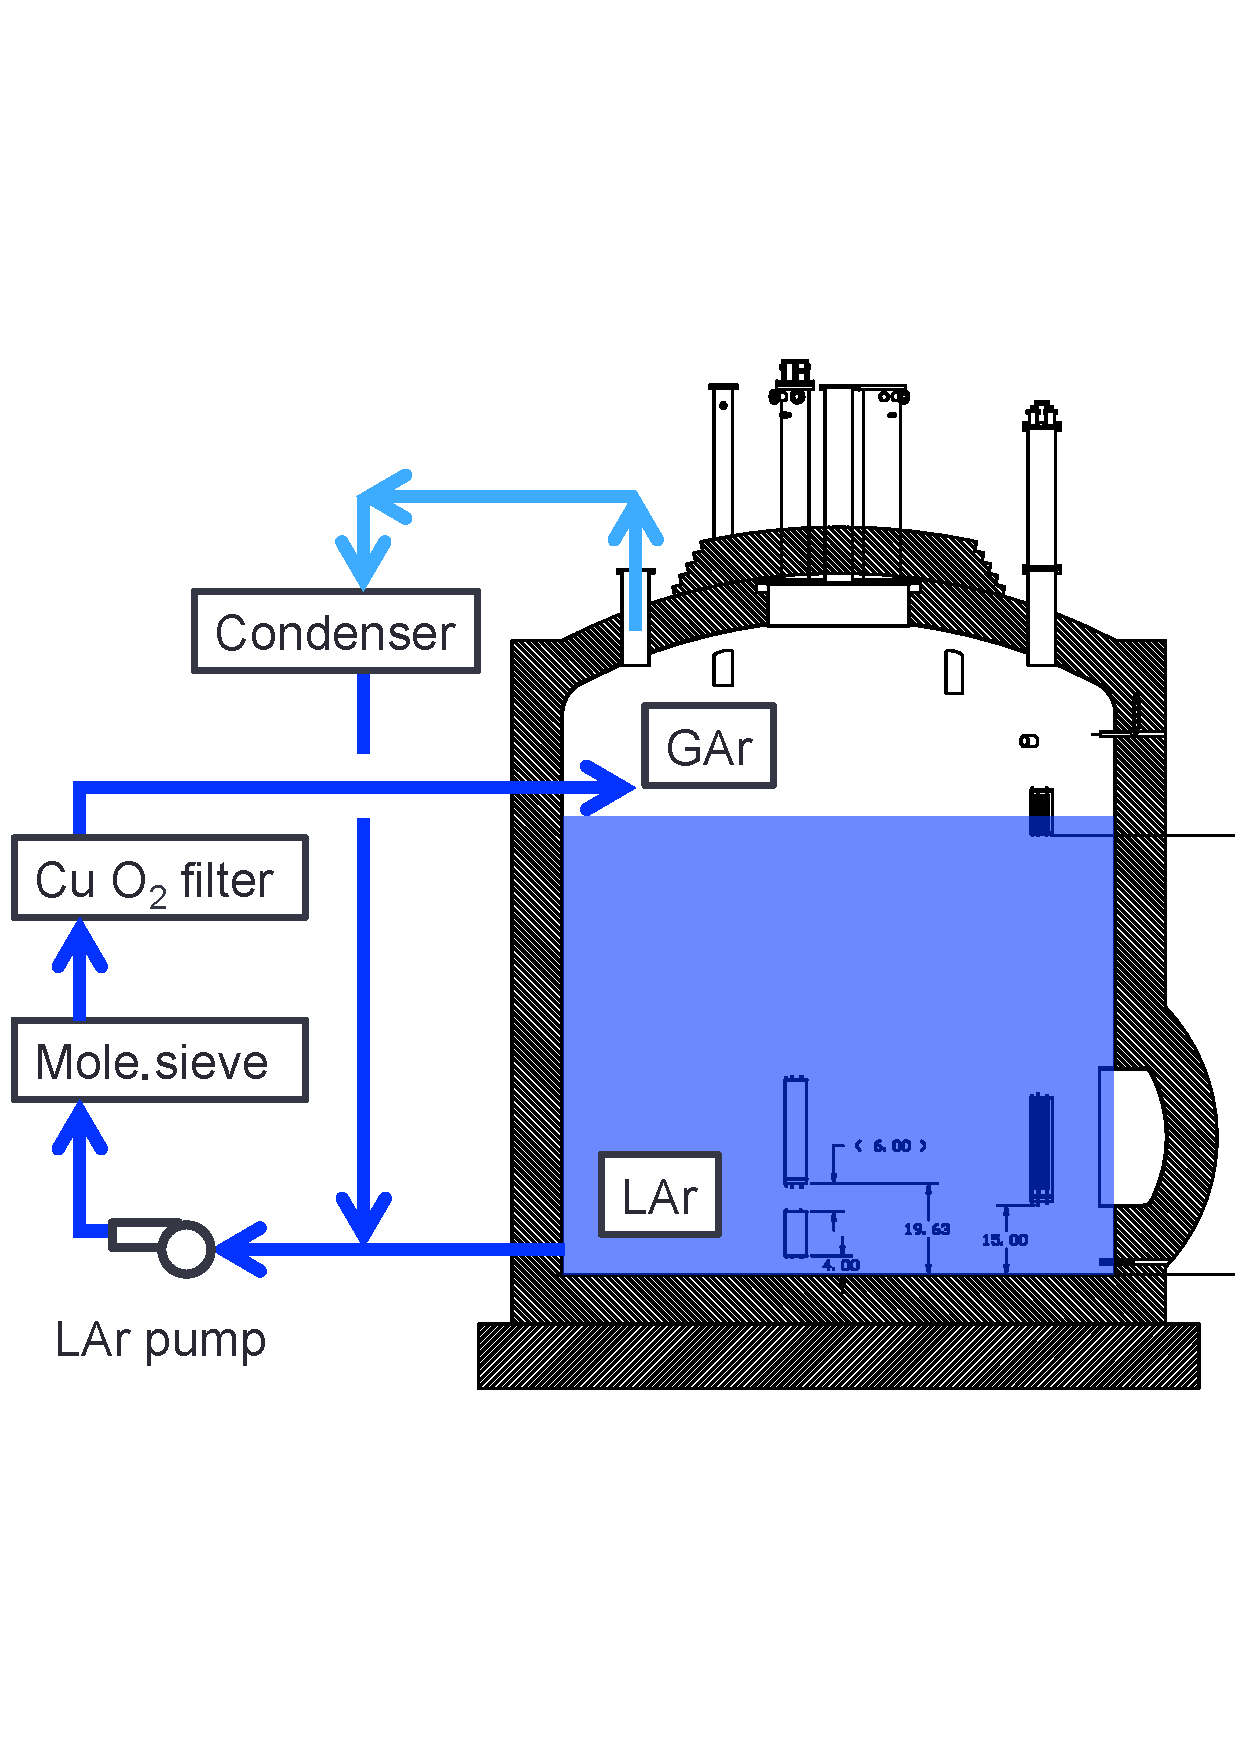
\includegraphics[width=10cm]{LAPDLiquidCirculation.pdf}
  \caption[Schematic showing the recirculation of the LAr during commissioning and operations of the Liquid Argon Purity Denomstrator.]{Schematic showing the recirculation of the LAr during commissioning and operations of the Liquid Argon Purity Denomstrator \cite{LAPD2014}.  Liquid is extracted from the bottom of the cryostat and pumped through the filters to remove any impurities which may have established in the medium.  Following the experience of previous R\&D with the MTS \cite{MTS2009a}, the recondensed liquid is passed through the purification system before being reintroduced to the main volume inside the cryostat.}
  \label{fig:LAPDLiquidCirculation}
\end{figure}

%----------------------------------------------------------------------------------------------------------------------------------------------------------------------------
\subsubsection{LAPD Outcomes}\label{sec:LAPDOutcomes}

LAPD successfully demonstrated achieving and maintaining the required LAr purity for a large neutrino detector is possible without the costly and challenging use of evacuation techniques, reaching purities upwards of 60~ppt O$_2$ equivalent.  The measured electron lifetimes over the course of a six week run is shown in Figure~\ref{fig:LAPDElectronLifetime}.  Lifetimes of up to 4~ms were recorded, greater than the DUNE requirement of 3~ms although utlitising a much smaller-scale cryostat.  Nonetheless, the success of LAPD has great significance for future LArTPCs, including the 35~ton, and was an important stage in the FNAL LAr test program.

\begin{figure}[ht]
  \centering
  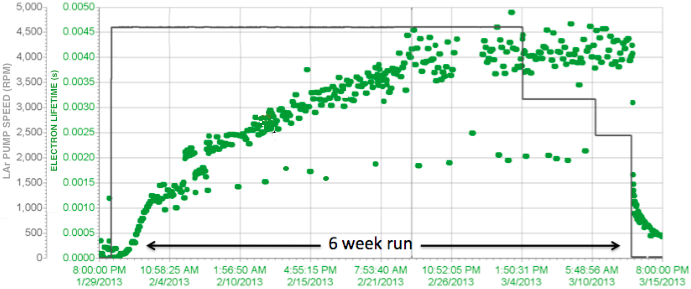
\includegraphics[width=12cm]{LAPDElectronLifetime.png}
  \caption[The electron lifetime achieved in the Liquid Argon Purity Demonstrator during a six week run.]{The electron lifetime achieved in the Liquid Argon Purity Demonstrator during a six week run.  Adapted from \cite{LAPD2014}.}
  \label{fig:LAPDElectronLifetime}
\end{figure}

%----------------------------------------------------------------------------------------------------------------------------------------------------------------------------
\subsection{LongBo}\label{sec:LongBo}

Following the successful LAPD runs, a futher phase involved the introduction of a small-scale TPC detector into the liquid argon \cite{LongBo2015}.  The detector is named LongBo (an upgrade from the smaller Bo test detector) and is cylindrical with 25~cm diameter and 2~m length.  It was positioned vertically in the LAPD cryostat, demonstrated in Figure~\ref{fig:LongBo}, and was equipped with a high voltage on the cathode to produce the drift field and three wire planes at the top of the detector for readout.  External scintillator counters were placed around the outer wall of the cryostat to provide triggers on through-going cosmic muons which may deposit charge in the detector.

\begin{figure}
  \centering
  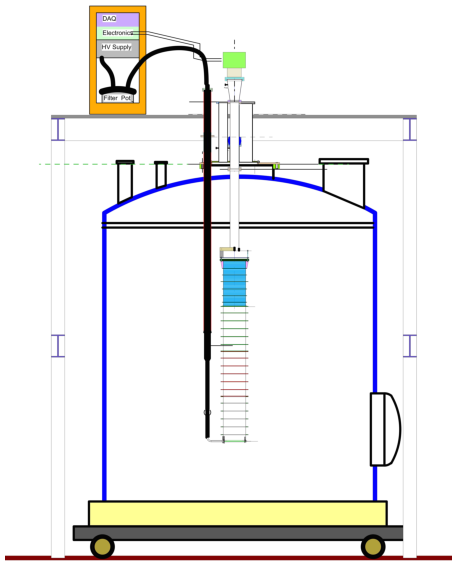
\includegraphics[width=8cm]{LongBo.pdf}
  \caption[The LongBo TPC detector shown within the Liquid Argon Purity Demonstrator Cryostat.]{The LongBo TPC detector shown within the Liquid Argon Purity Demonstrator Cryostat \cite{LongBo2015}.  The black tube represents the high voltage feedthrough to the cathode at the bottom of the TPC.}
  \label{fig:LongBo}
\end{figure}

LongBo was the first LArTPC experiment to utilise `cold readout' electronics to amplify and shape the signal at the front end.  An early version of the ASICs being developed for MicroBooNE were used to read out 16 of the 144 channels, with the remaining using preamplifiers made with discrete circuitry.  At the drift field of 350~V/cm, the signal/noise ratio, a useful number in quantifying the electronics, was around 30, with the channels read out by the ASICs reporting values up to 1.4 times larger.

The LAPD/LongBo experiment successfully maintained similar LAr purities than without the presence of the detector, as predicted by the results of the MTS.  By using TPC data, it was also possible to make measurements of the electron lifetime from through-going muons (using Equation~\ref{eq:ElectronLifetime}).  A comparison between the measured values from the purity monitors and the TPC data may be found in Figure~\ref{fig:LongBoPurity}.  A reasonable agreement is observed between these complimentary measurements with values between 6~ms and 14~ms reported, with 95\% confidence.  These promising results confirmed designing and operating a LArTPC within a non-evacuable cryostat is viable and contributed to the development of the LAr program towards the DUNE far detector, with the 35~ton experiment the next stage.

\begin{figure}
  \centering
  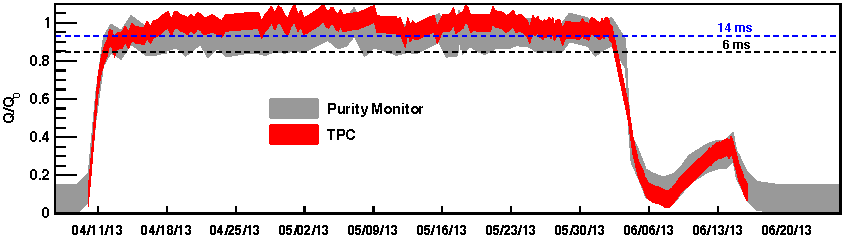
\includegraphics[width=14cm]{LongBoPurity.pdf}
  \caption[The LAr purity within the Liquid Argon Purity Demonstrator cryostat with the LongBo TPC present, measured using both data from the detector and information from the purity monitors.]{The LAr purity within the Liquid Argon Purity Demonstrator cryostat with the LongBo TPC present, measured using both data from the detector and information from the purity monitors \cite{LongBo2015}.}
  \label{fig:LongBoPurity}
\end{figure}

%----------------------------------------------------------------------------------------------------------------------------------------------------------------------------
\section{35~ton Experiment: Phase~I}\label{sec:35tonPhaseI}

The scale of the cryostats required for the DUNE experiment are such that constructing them as flat plane vessels 1.5~km underground would be unfeasibily expensive and pose huge engineering challenges.  Following the success of LAPD (discussed in Section~\ref{sec:LAPD}), which eliminates the requisite to evacuate the cryostat prior to filling, the LBNE collaboration decided to utilise membrane cryostat technology well established in the liquified natural gas (LNG) industry.  The 35~ton \cite{35tonPhaseI2014Cryostat,35tonPhaseI2014,35tonPhaseI2015} was therefore employed to demonstrate the application of a membrane cryostat to a LAr experiment and was the only planned prototype for LBNE.  The DUNE project has maintained this design choice and the 35~ton has since become a recognised and integral part of the collaboration, providing the first test of the technologies envisioned for the eventual far detector.

The 35~ton croystat was constructed in 2012 at PC4, a former proton facility in a decomissioned beamline, at Fermilab.  It has operated in two phases: Phase~I (December 2013 -- February 2014) was proposed to demonstrate the membrane cryostat technology with just the cryostat and purification systems; Phase~II (February 2016 -- April 2016) contained a small-scale DUNE-style detector to validate the integrated system and affirm the detector design elements.  The Phase~I run is the subject of Section~\ref{sec:35tonPhaseI} whilst Phase~II is considered in detail in Section~\ref{sec:35tonPhaseII}.

The 35~ton is the first membrane cryostat used for scientific purposes and the first overall constructed in the United States.  It is also the first designed to contain LAr, which is around three times denser than LNG.  The initial aims of the project (Phase~I) include to demonstrate the feasibility of the cryostat technology for LAr, including thermal performance and leak tightness, and to show the required LAr purity may be acheived without evacuation and maintained through the use of the filtration system developed and validated by the MTS and LAPD.  This first phase will be discussed in this section; the 35~ton cryostat and filling procedures will be described in Sections~\ref{sec:35tonCryostat} and~\ref{sec:35tonFilling} respectively before outcomes of the experiment are presented in Section~\ref{sec:35tonPhaseIOutcomes}.

%----------------------------------------------------------------------------------------------------------------------------------------------------------------------------
\subsection{The 35~ton Cryostat}\label{sec:35tonCryostat}

An overview of the 35~ton cryostat is shown in Figure~\ref{fig:35tonCryostat}.  It contains a concrete shell within which the membrane cryostat is constructed from 2~mm think stainless steel panels.  An insulated region between these two segments reduces heat leaking.  The roof consists of two plates; Plate A is flat with insulation and membrane beneath and Plate B contains all penetrations and services.  Relevant properties of the 35~ton cryostat are listed in Table~\ref{tab:35tonCryostat}.

\begin{figure}
  \centering
  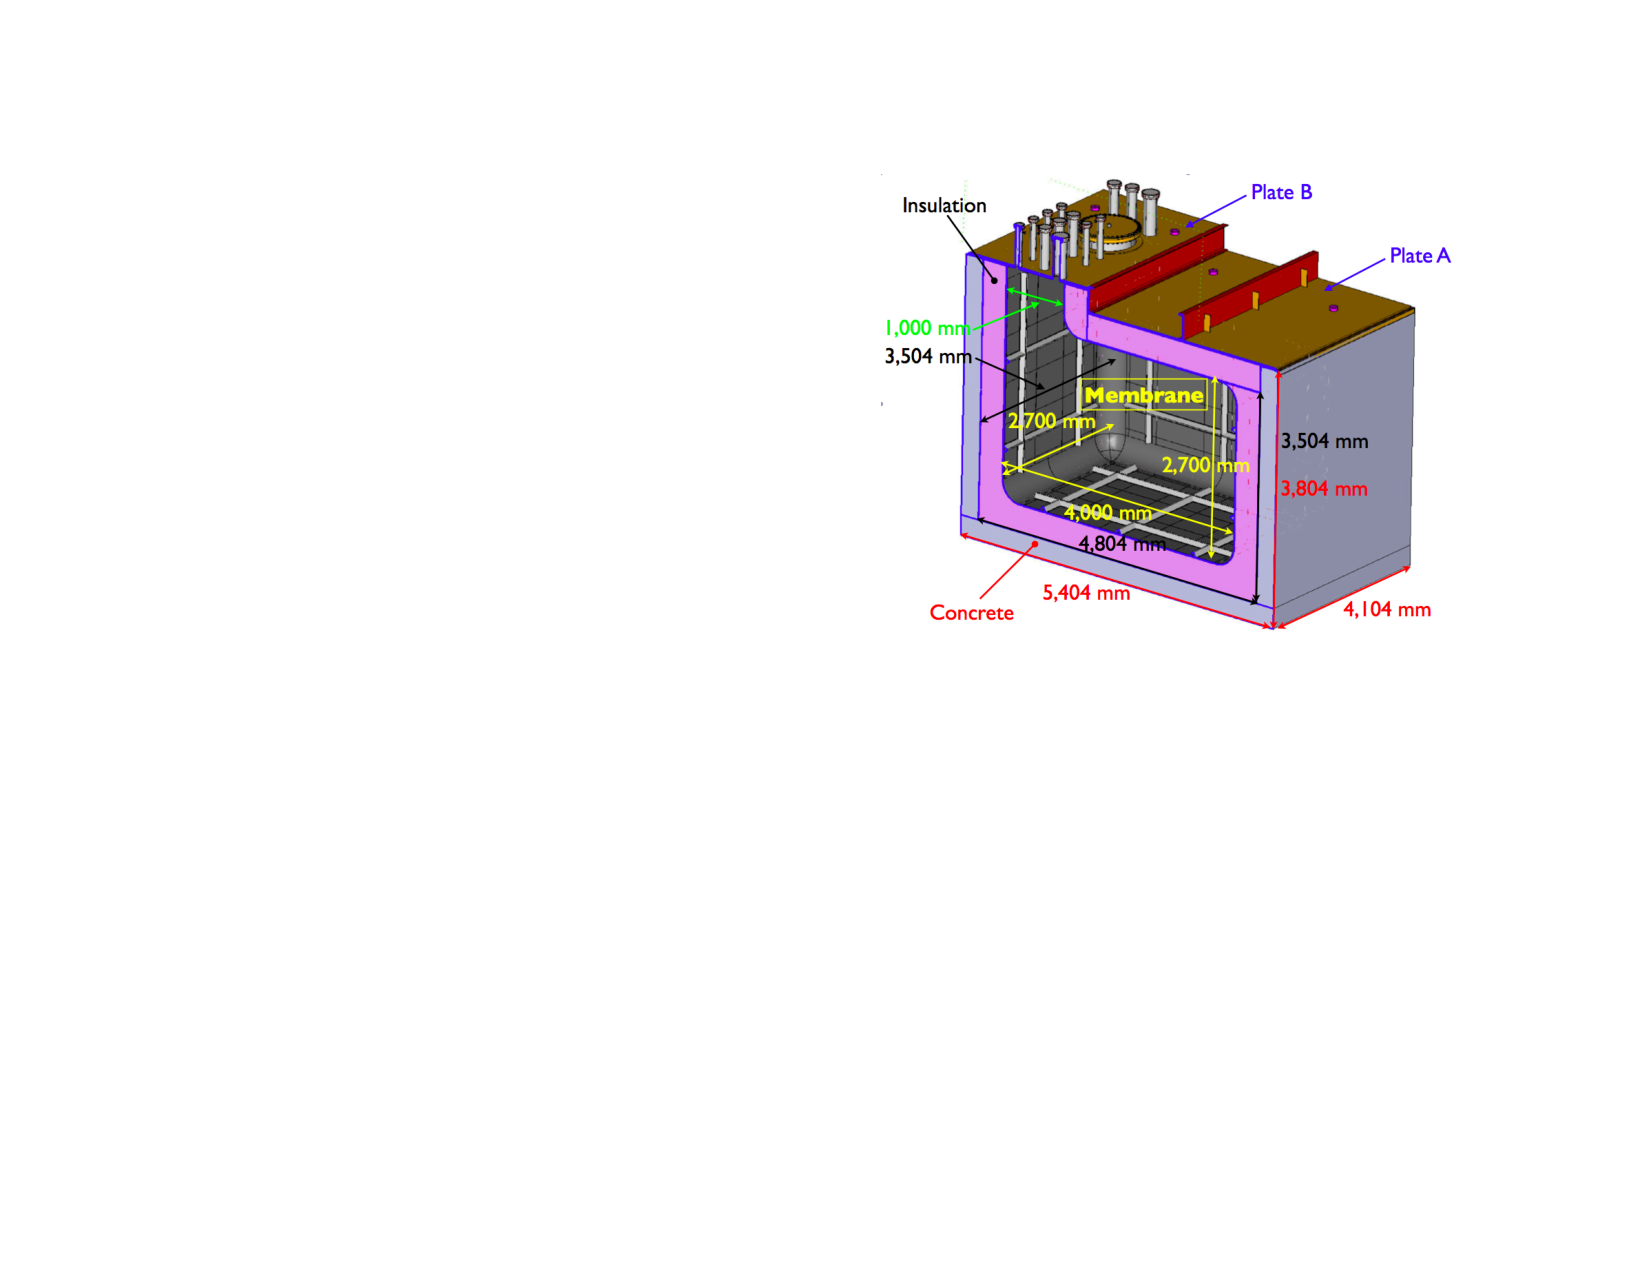
\includegraphics[width=10cm]{35tonCryostat.pdf}
  \caption[The 35~ton cryostat.]{The 35~ton cryostat \cite{35tonPhaseI2015}.}
  \label{fig:35tonCryostat}
\end{figure}

\begin{table}
  \caption[Details and dimensions of the 35~ton cryostat.]{Details and dimensions of the 35~ton cryostat \cite{35tonPhaseI2015}.}
  \label{tab:35tonCryostat}
  \centering
  \begin{tabular}{ l l }
    \toprule
    Parameter & Value \\
    \midrule
    Cryostat volume           & 29.16~m$^3$ \\
    LAr total mass            & 38.6~metric tons \\
    Depth of LAr              & 2.565~m (11\% total ullage) \\
    Inner dimensions          & 4.0~m (length) $\times$ 2.7~m (width) $\times$ 2.7~m (height) \\
    Insulation                & 0.4~m polyurethane foam \\
    Primary membrane          & 2.0~mm thick corrugated stainless steel \\
    Secondary barrier system  & 0.1~mm thick fiberglass \\
    Vapor barrier             & 1.2~mm thick carbon steel \\
    Steel reinforced concrete & 0.3~m thick layer \\
    LAr temperature           & $89\pm1$~K \\
    Operating gas pressure    & 70~mBar \\
    Design pressure           & 207~mBar \\
    Heat leak                 & $<13$~W/m$^2$ \\
    Leak tightness            & $1\times10^{-6}$~mBar$\cdot$litre/s \\
    \bottomrule
  \end{tabular}
\end{table}

The 35~ton was constructed physically nearby the Liquid Argon Purity Demonstrator in order to utilise existing infrastructure.  It is connected to the LAPD tank, which may be used to store LAr before transferring to the 35~ton, and uses the filtration setup designed and validated by the MTS and LAPD.  This network is shown schematically in Figure~\ref{fig:35tonLAPD}.  Unlike in LAPD, the pumps used in the 35~ton to circulate the LAr through the purification system are within the liquid but the framework operates in a similar way.  An identical condenser is also employed above the cryostat to cool boiled off gaseous argon which is returned to the bottom of the cryostat, nearby the pumps which subsequently extract the liquid for purification.

\begin{figure}
  \centering
  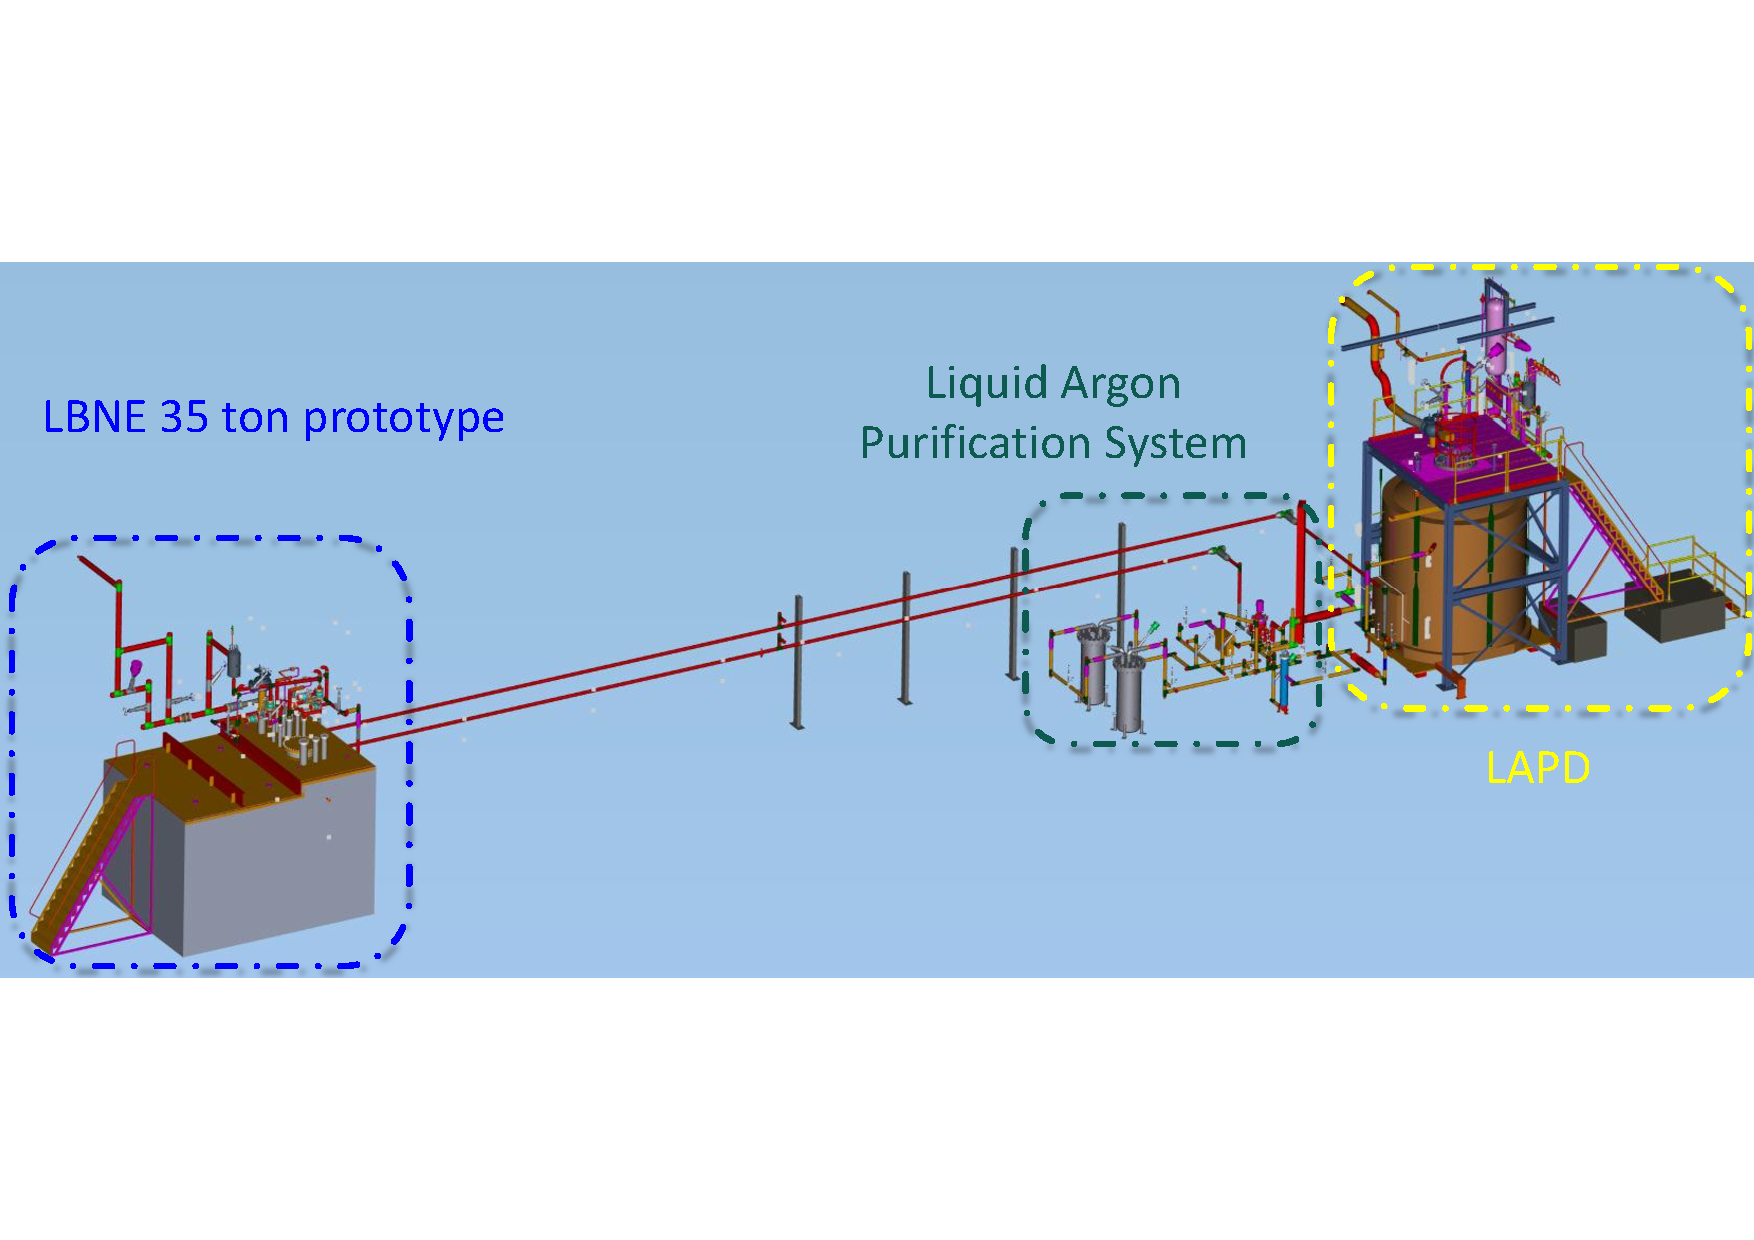
\includegraphics[width=14cm]{35tonLAPD.pdf}
  \caption[The network linking the 35~ton cryostat, the Liquid Argon Purity Demonstrator and the purification system at PC4, Fermilab.]{The network linking the 35~ton cryostat, the Liquid Argon Purity Demonstrator and the purification system at PC4, Fermilab \cite{35tonPhaseI2014}.}
  \label{fig:35tonLAPD}
\end{figure}

The cryogenic environment is monitored and controlled using standard detectors including temperature sensors, pressure transducers, flow meters and level sensors along with a suite of commercial gas analysers.  The height of the volume is instrumented with four purity monitors, two large and two small, with an additional long monitor positioned after the filters, as with LAPD.  Also as previously, the vertical temperature profile in the cryostat is monitored at 23~cm intervals with temperature detectors suspended on a chain.

%----------------------------------------------------------------------------------------------------------------------------------------------------------------------------
\subsection{Filling the 35~ton}\label{sec:35tonFilling}

The 35~ton cryostat is filled in a similar way to the Liquid Argon Purity Demonstrator, described in Section~\ref{sec:FillingLAPD}.  Initially, a piston purge with warm gaseous argon is performed to remove atmospheric impurities before closing off the vents and redirecting argon at the top of the cryostat through the filters for purification.  The impurity concentrations for this stage of filling are shown in Figure~\ref{fig:35tonGasFilling}.  Before filling with liquid, the cryostat is cooled in an attempt to reduce outgassing and to create an appropriate environment in which to introduce LAr.  This is achieved by injecting LAr through a spray at the top of the cryostat which generates a turbulent mixing of cold gas within the cryostat and gradually cools the walls of the vessel.  Following this, LAr is transferred from LAPD into the 35~ton; this is conducted in two stages since the 35~ton is slightly larger than LAPD.  The cooldown and LAr filling stages are shown in Figure~\ref{fig:35tonLiquidFilling}.

\begin{figure}
  \centering
  \begin{subfigure}[t]{0.48\linewidth}
    \centering
    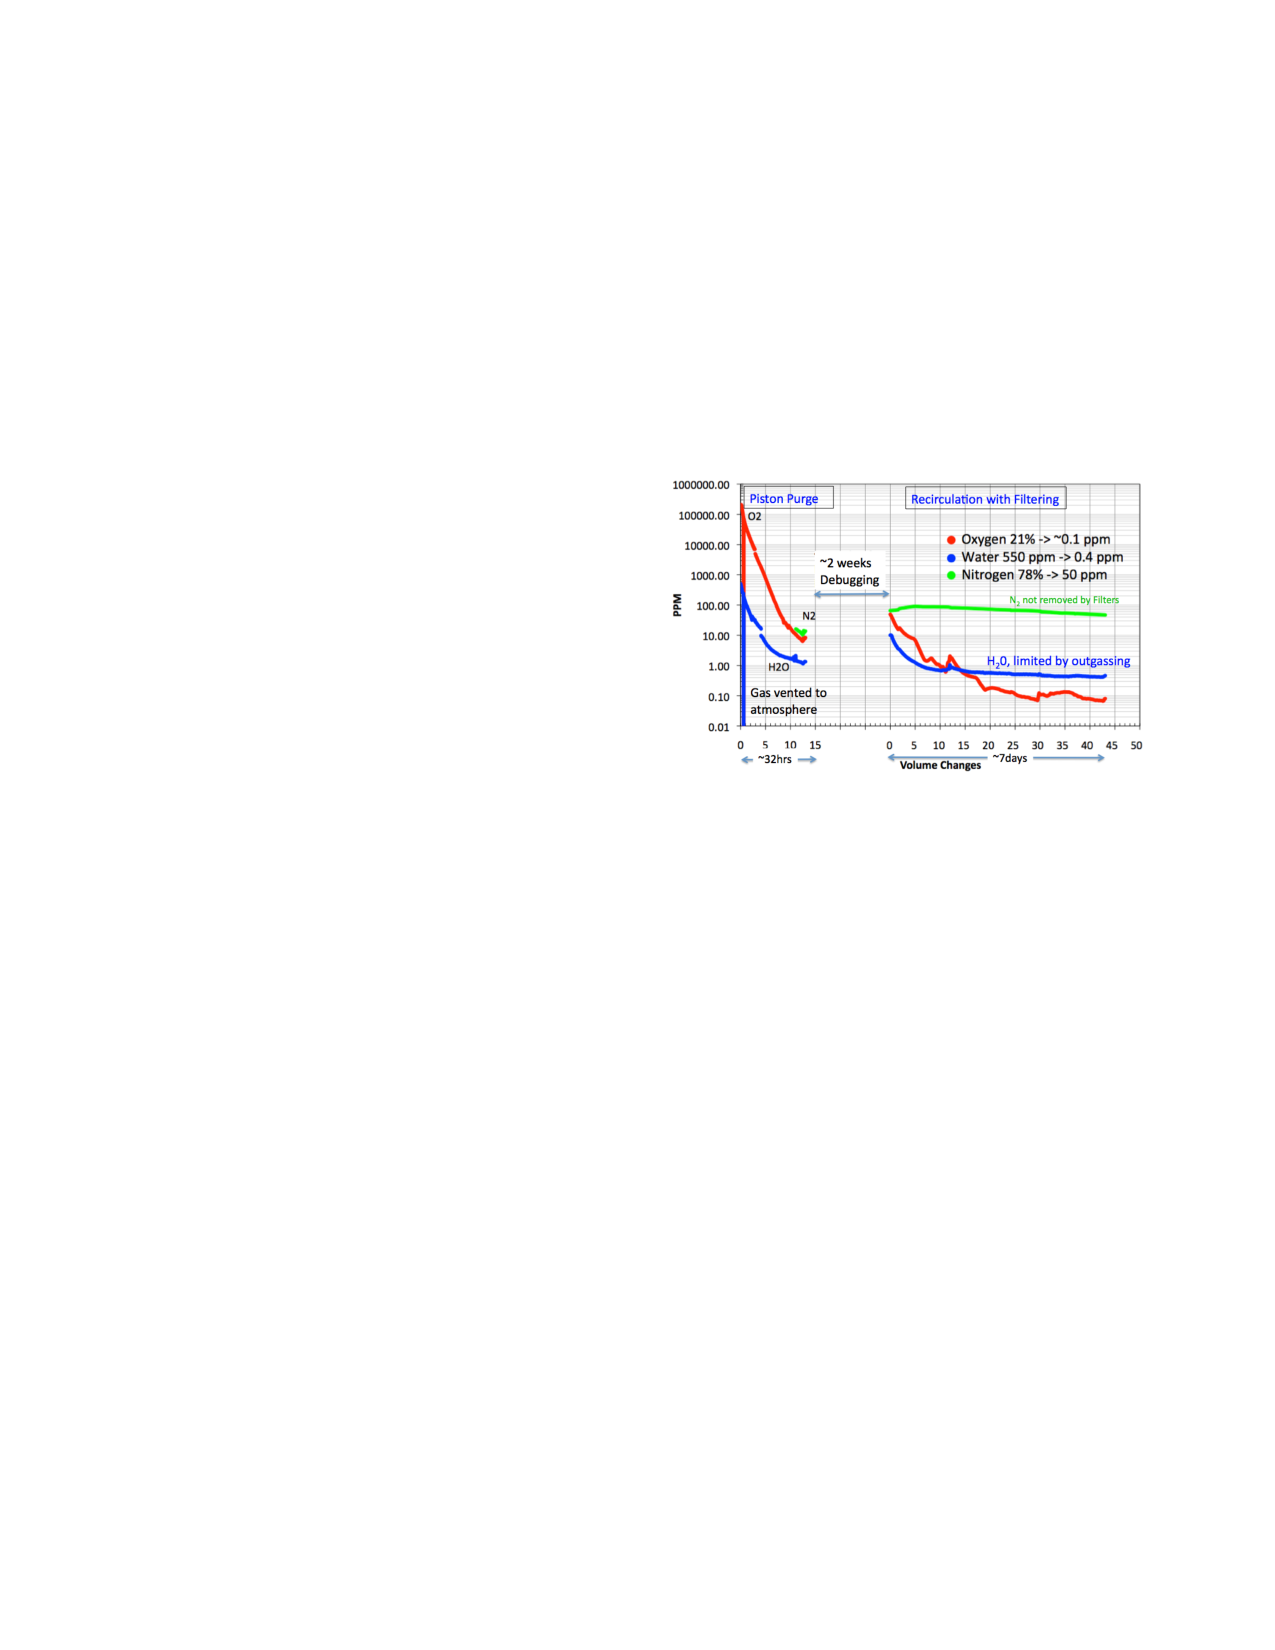
\includegraphics[width=0.98\textwidth]{35tonGasFilling.pdf}
    \caption{Gas filling.}
    \label{fig:35tonGasFilling}
  \end{subfigure}
  \hfill
  \begin{subfigure}[t]{0.48\linewidth}
    \centering
    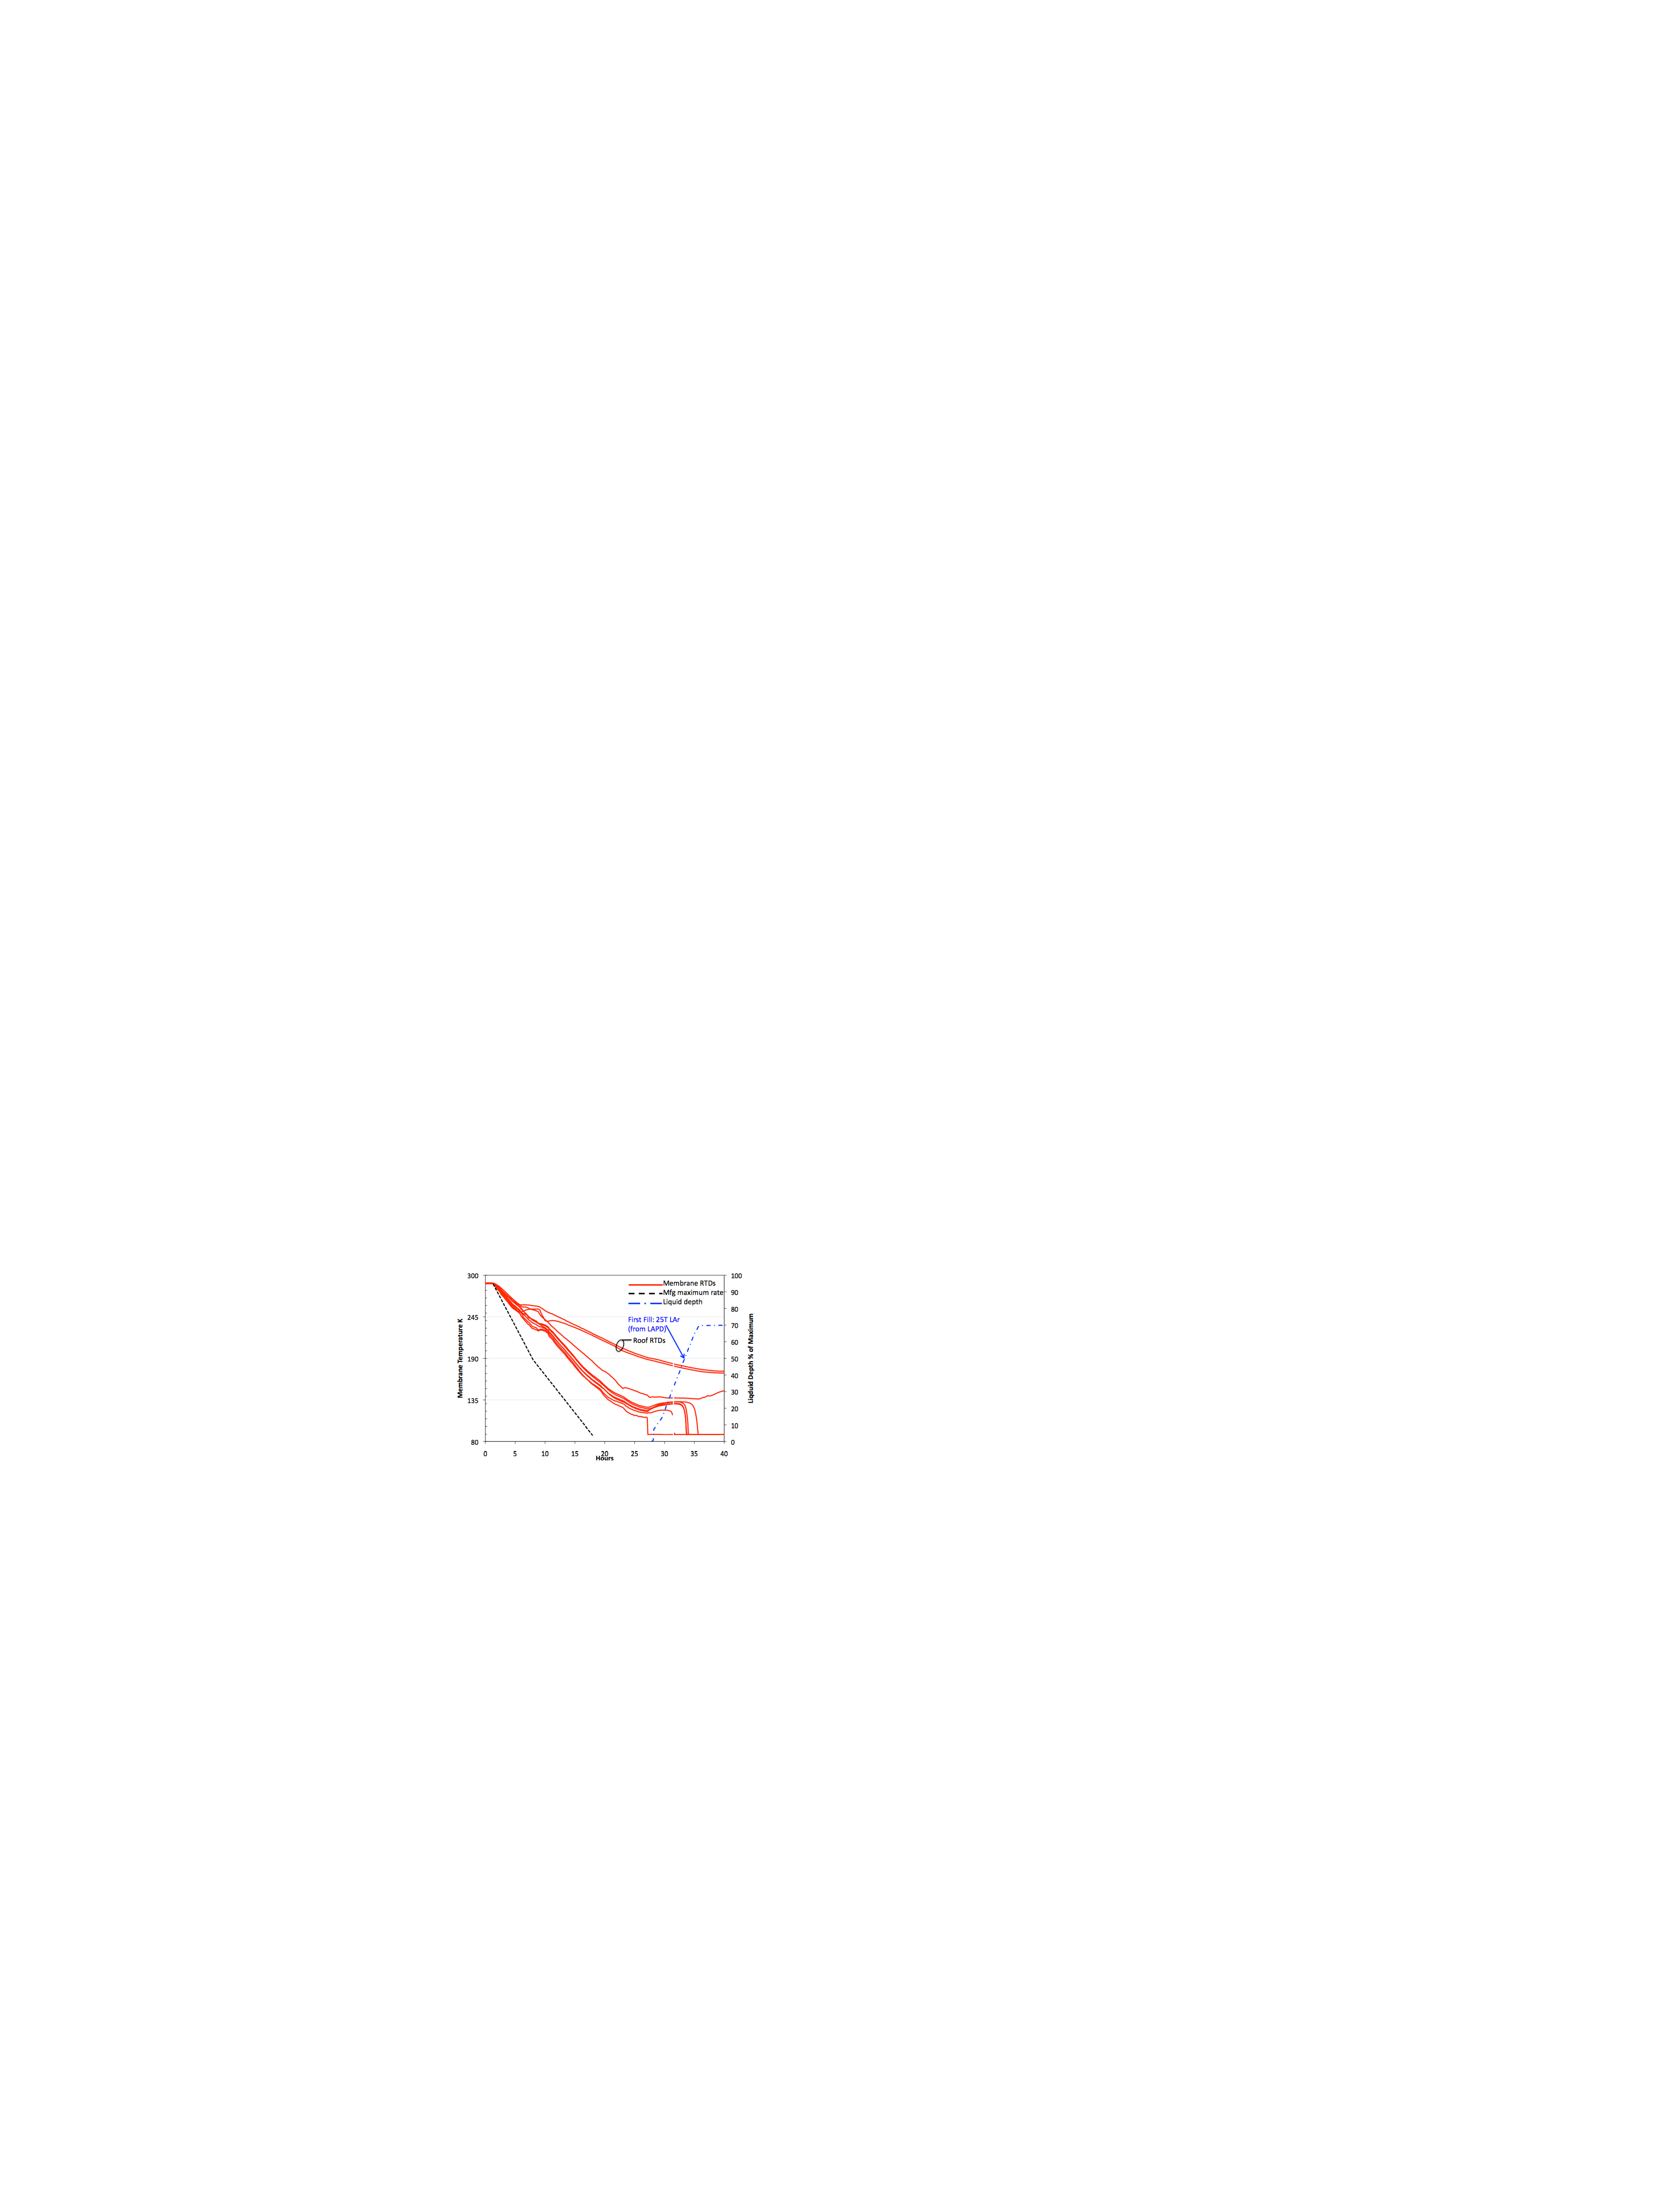
\includegraphics[width=0.98\textwidth]{35tonLiquidFilling.pdf}
    \caption{Liquid filling.}
    \label{fig:35tonLiquidFilling}
  \end{subfigure}
  \caption[Filling the 35~ton cryostat in four stages: piston purge, gas recirculation, cooldown and liquid filling.]{Filling the 35~ton cryostat in four stages: piston purge, gas recirculation, cooldown, liquid filling \cite{35tonPhaseI2015}.  The gas filling is shown in Figure~\ref{fig:35tonGasFilling} and involves using a piston purge to fill the tank with warm gaseous argon before circulating this gas through the filtration system.  Cooldown and liquid filling is demonstrated in Figure~\ref{fig:35tonLiquidFilling}, which shows the falling temperature of the crysotat as a result of the injection of liquid argon through the cooldown sprayers and the rising LAr level as the cryostat is filled from LAPD.}
  \label{fig:35tonFilling}
\end{figure}

%----------------------------------------------------------------------------------------------------------------------------------------------------------------------------
\subsection{Outcomes of Phase~I}\label{sec:35tonPhaseIOutcomes}

The 35~ton successfully demonstrated the feasibility of membrane cryostats for use with LAr and additionally showed the required LAr purity for future multi-kton LArTPC experiments may be achieved and held in such a vessel.  The lifetime over the course of the $\sim2$~month run, along with external changes to the system, is comprehensively summarised in Figure~\ref{fig:35tonPhaseIElectronLifetime}.

\begin{figure}
  \centering
  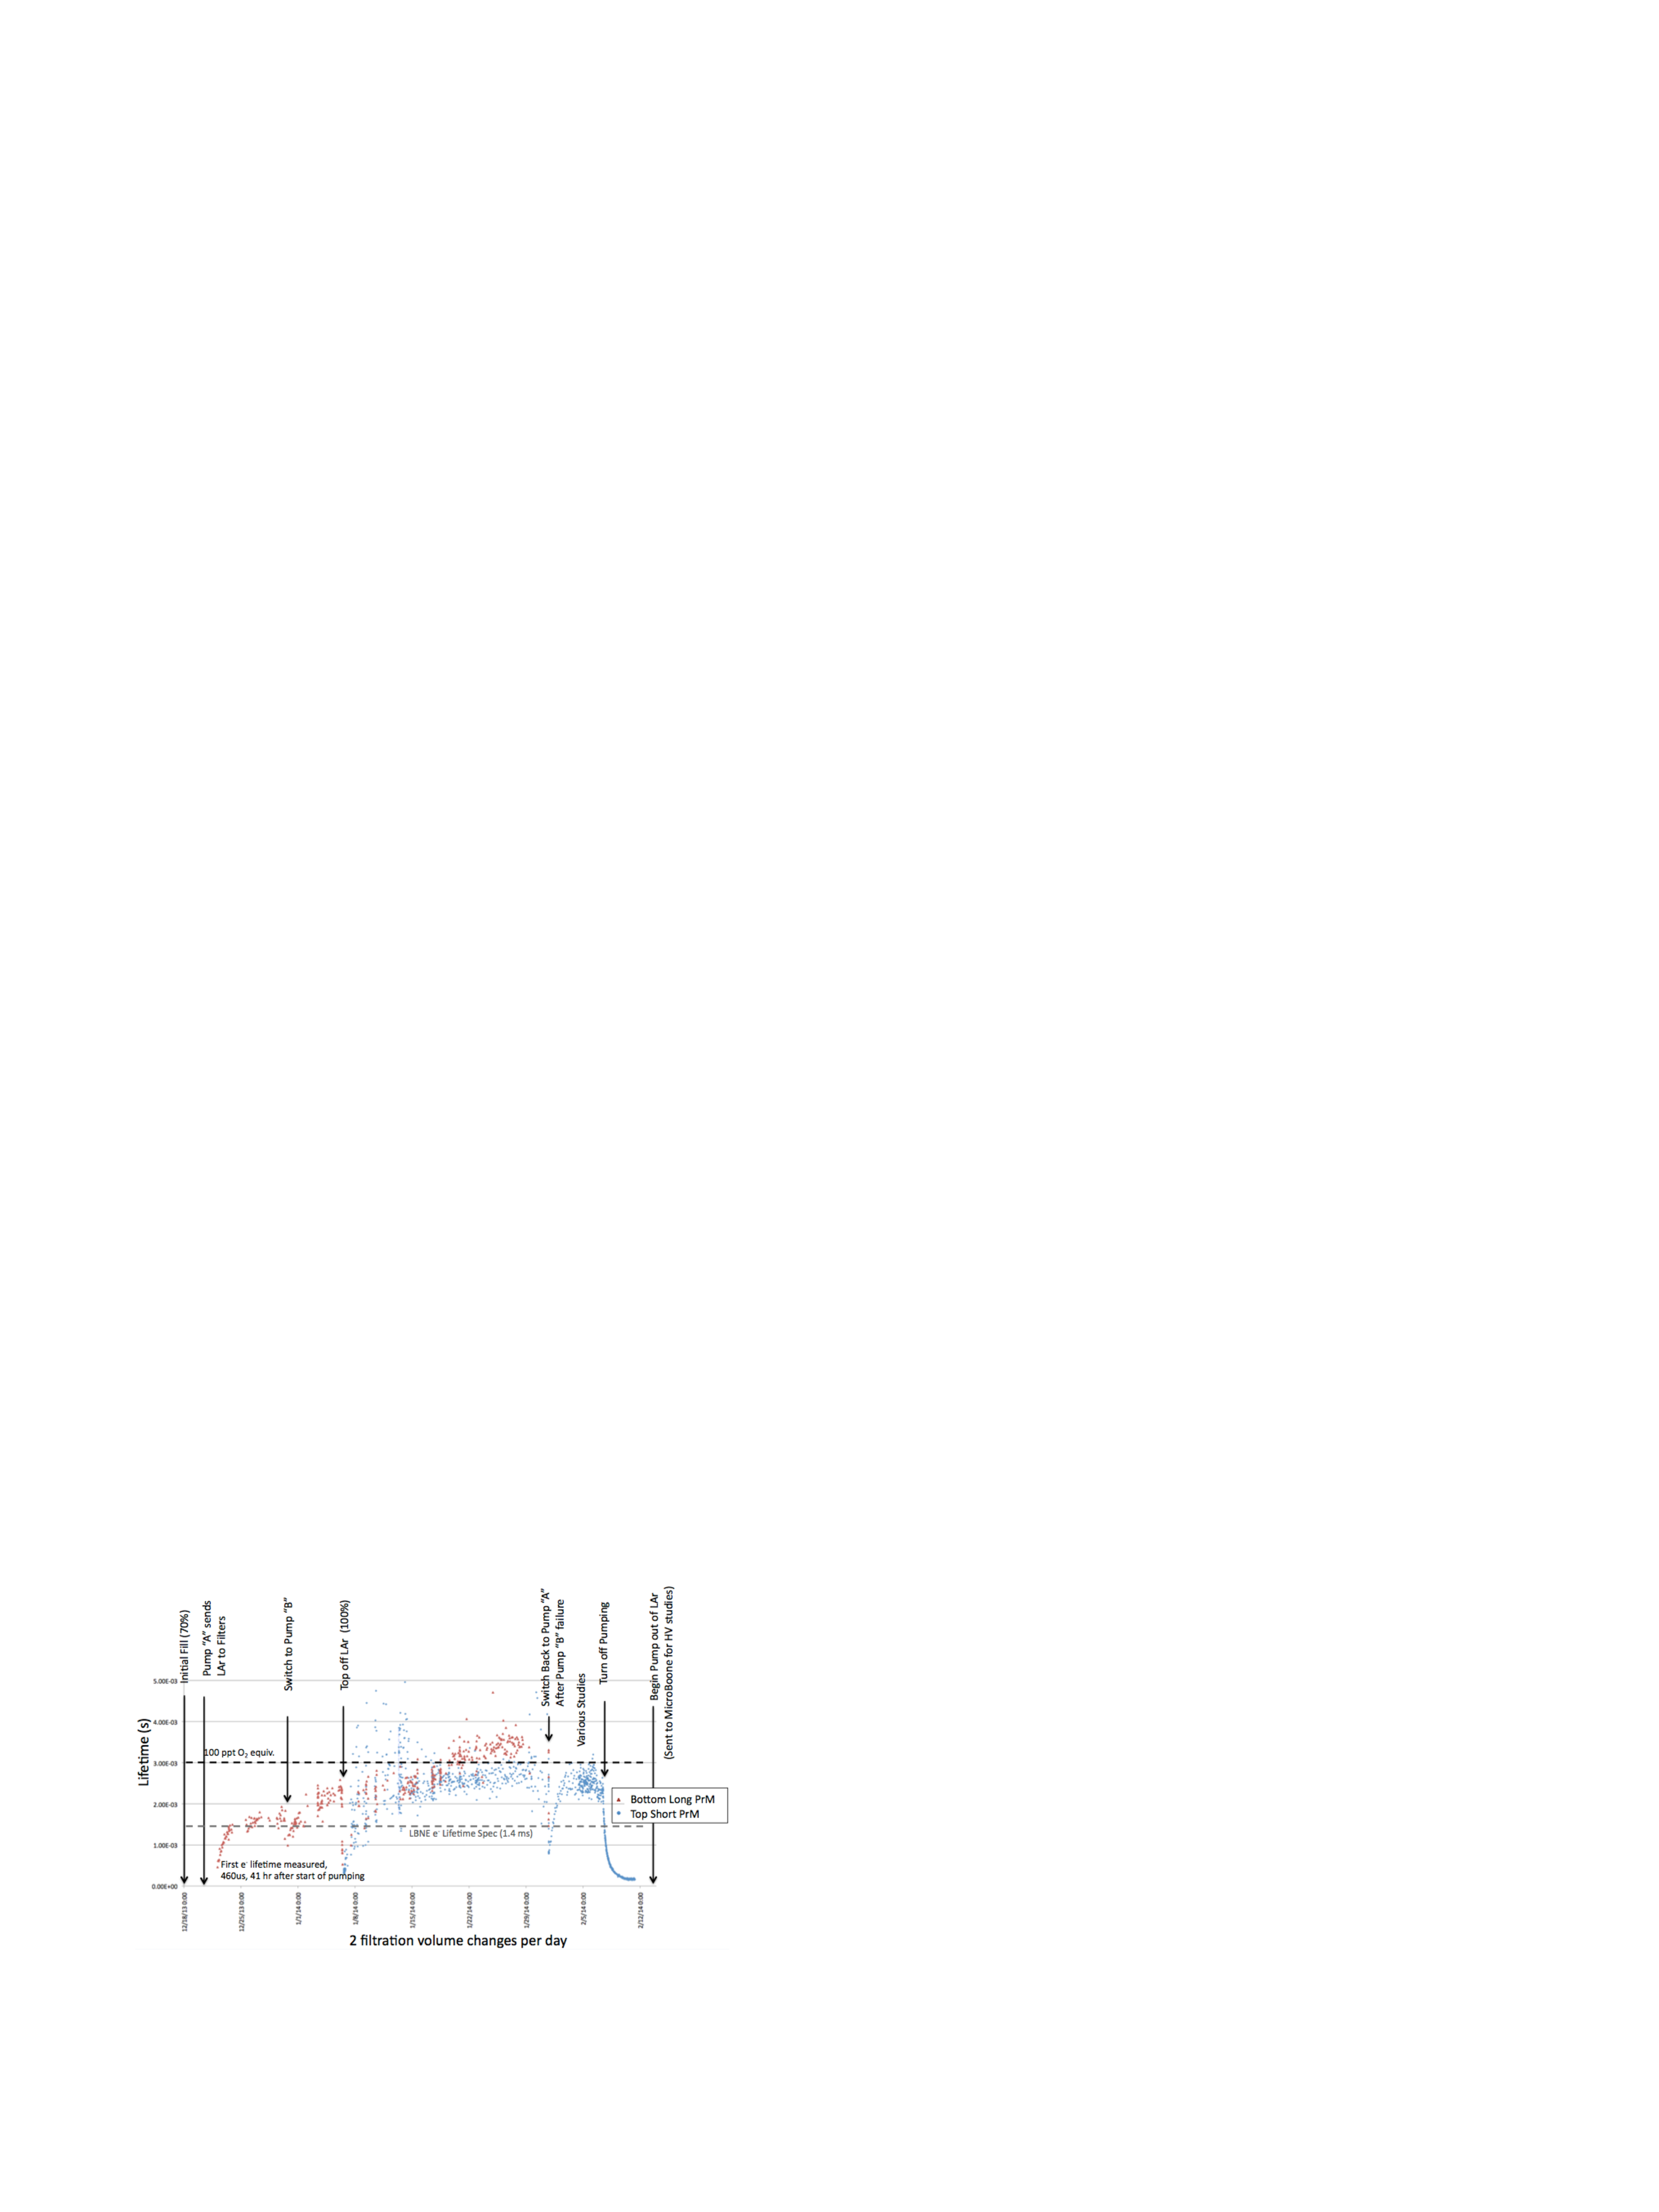
\includegraphics[width=14cm]{35tonPhaseIElectronLifetime.pdf}
  \caption[The electron lifetime in the 35~ton cryostat measured by two purity monitors over the course of the two month Phase~I run.]{The electron lifetime in the 35~ton cryostat measured by two purity monitors over the course of the two month Phase~I run \cite{35tonPhaseI2014}.  The measurements correspond to different positions in the cryostat, with the red points showing purity measurements at the bottom and blue points near the top.  Major external factors affecting the observed LAr purity are shown at the top of the figure.  The old LBNE requirement of 1.4~ms is noted as a dashed grey line; DUNE now requires 3~ms lifetime, equivalent to 100~ppt O$_2$ and illustrated by the black dashed line.}
  \label{fig:35tonPhaseIElectronLifetime}
\end{figure}

The lifetime is observed to reach and remain at the DUNE requirement for a good period of time; this is a major achievement in the context of the future of LArTPC experiments.  Dips in the purity were observed when topping up the croystat after initially filling one LAPD volume and when switching between the two pumps installed to extract the liquid for purification.  In both cases, good purity is recovered after a few volume exchanges.

The same variations of lifetime on temperature were observed as previously noticed in the MTS and LAPD, suggesting a genuine effect dependent on the ambient conditions.  Addtionally, during gas circulation a leak was found and fixed in a seal and, during cold operations, a leak developed in the argon cryo-piping as the dielectric breaks necessary to electrically isolate the cryostat from the building were not leak tight at cryogenic temperatures.  All associated 35~ton experience is useful as progress continues to larger and more complicated LAr cryostats.

The success of the 35~ton was exploited by utilising the existing setup for a second run, involving a small-scale DUNE-style detector.  This would be the first time a membrane cryostat would facilitate a detector and is the next stage along in prototyping the DUNE far detector.

%----------------------------------------------------------------------------------------------------------------------------------------------------------------------------
\section{35~ton Experiment: Phase~II}\label{sec:35tonPhaseII}

The first (and to date, only) particle detector housed within a membrane cryostat was the 35~ton Phase~II.  Following the positive outcomes of the 35~ton Phase~I (discussed in Section~\ref{sec:35tonPhaseI}), it is natural to extend operations to include a prototype DUNE detector.  The initial aims of the 35~ton Phase~II experiment were to develop, build and install a working TPC within the existing cryostat and infrastructure and make measurements of particle interactions induced by cosmic muons whilst demonstrating the required LAr purity is still maintained within a integrated system.  The far detector design was heavily constrained by construction, transport, assembly, time and cost requirements and prototyping is essential to demonstrate the required spatial, time and energy resolution, signal-to-noise performance, detection efficiency and uptime may be achieved.

The operation of the second 35~ton phase will be discussed in detail in this section.  An overview of the detector is provided in Section~\ref{sec:35tonDetector} before the data acquisition from the detector elements is discussed in Section~\ref{sec:35tonDataAcquisition}.  The custom camera system developed at Sheffield for detecting dielectric breakdown of the LAr is the subject of Section~\ref{sec:SheffieldCameras}.  Finally, the period of data taking is outlined in Section~\ref{sec:35tonPhaseIIRun} before outcomes of the project are presented in Section~\ref{sec:35tonPhaseIIOutcomes}.

%----------------------------------------------------------------------------------------------------------------------------------------------------------------------------
\subsection{The 35~ton Detector}\label{sec:35tonDetector}

A cutaway view of the 35~ton cryostat showing the detector installed in shown in Figure~\ref{fig:35tonDetector}.  The detector elements are designed to prototype as many features of the DUNE far detector as possible (shown in Figure~\ref{fig:DUNEFarDetectorDesign}).  The readout is performed by four APAs with wrapped induction wires and cold front end electronics (amplifiers and digitisers) which read out multiple drift regions simultaneously.  Embedded within the APAs are photon detectors, representing three difference design choices, to trigger on scintillation light.  The drift field is enabled by cathodes at either end of the TPC.  A flange placed on Plate A facilitates a warm/cold interface through which all electrical signals and the high voltage (HV) feedthrough pass.  Surrounding the walls of the cryostat are over 100 scintillation paddles (Cosmic Ray Counters, CRCs) to provide additional triggers from through-going cosmic muons.

\begin{figure}
  \centering
  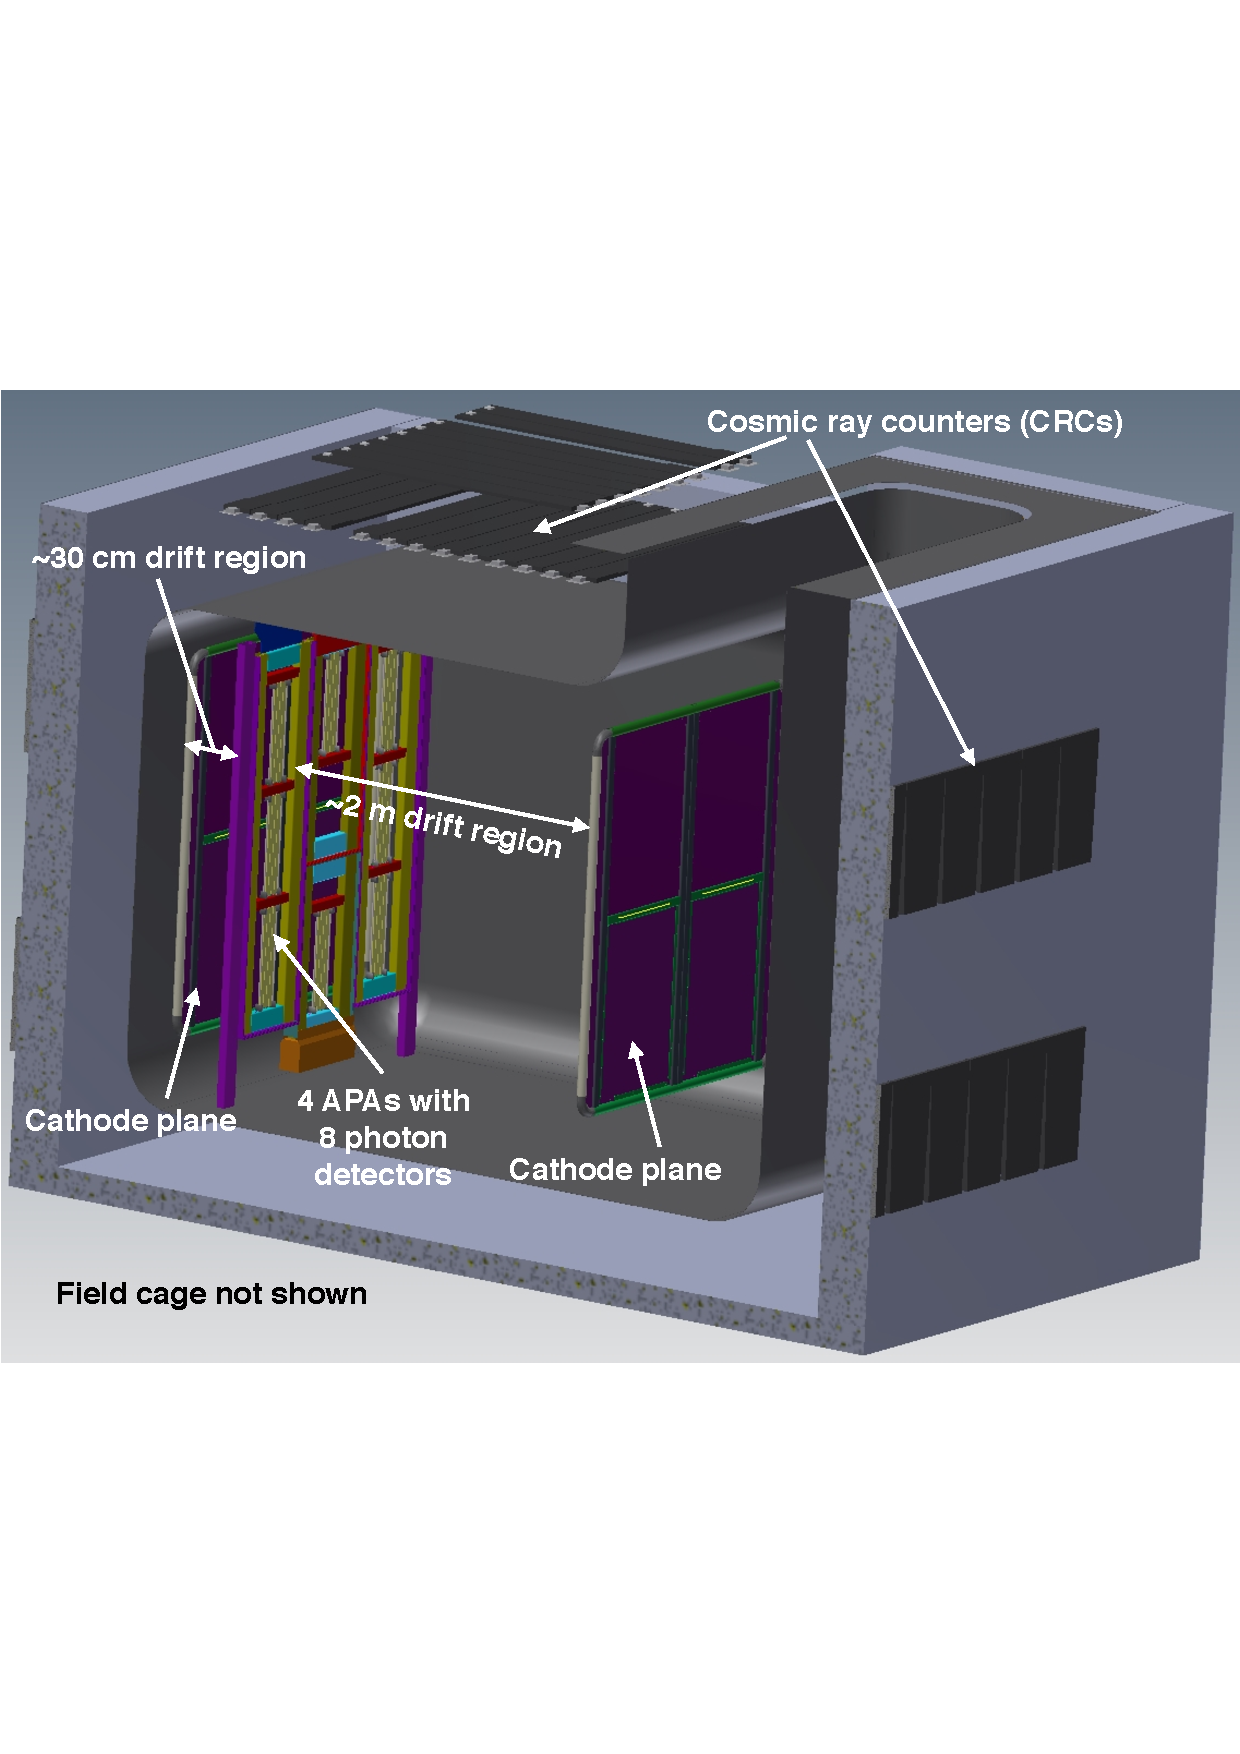
\includegraphics[width=10cm]{35tonDetector.pdf}
  \caption[The 35~ton detector operated during Phase~II of the 35~ton program.]{The 35~ton detector operated during Phase~II of the 35~ton program \cite{35tonPhaseINeutrino2014}.}
  \label{fig:35tonDetector}
\end{figure}

The three main detector components, the TPC, photon detectors and CRCs, are discussed in the following sections.  A photograph of the partially installed detector is shown in Figure~\ref{fig:35tonPhoto} highlighting most of the detector during construction.

\begin{figure}
  \centering
  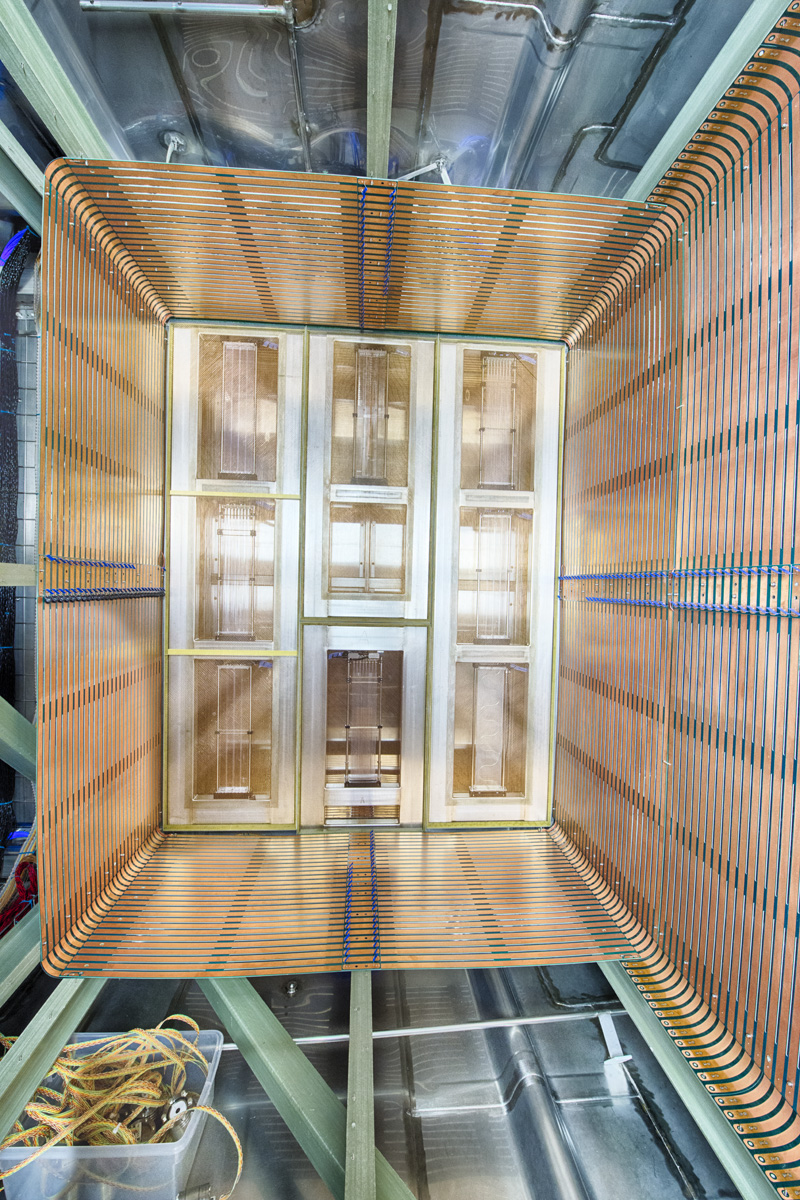
\includegraphics[width=11cm]{35tonPhoto.jpg}
  \caption[Photograph of the partially installed 35~ton detector.]{Photograph of the partially installed 35~ton detector \cite{VMS}.  The four APAs, with the embedded photon detectors, are visible and the field cage is under construction.  Cameras and cold cabling from the Sheffield Camera System, the subject of Section~\ref{sec:SheffieldCameras}, may be observed in a box, prior to installation, at the bottom of the photo.}
  \label{fig:35tonPhoto}
\end{figure}

%----------------------------------------------------------------------------------------------------------------------------------------------------------------------------
\subsubsection{TPC}\label{sec:35tonTPC}

The 35~ton TPC is very similar to the DUNE single phase design introduced in Section~\ref{sec:DUNESinglePhase}.  It has a module form, with multiple APAs reading out separate drift volumes, and two drift regions: the `long drift region' of length 2.26~m and the `short drift region', around 0.30~m long.  These were chosen to ensure the longest possible drift region in order to closely resemble the far detector drift distances, whilst ensuring the double-sided readout of the APAs may be tested.  Four APAs are used with a very similar design to that demonstrated in Figure~\ref{fig:DUNEFarDetectorAPA}; each contains two wrapped induction views with a grid and collection plane on each face.  The main difference between the APAs tested in the 35~ton and the current DUNE far detector design is the physical dimensions of the frames and the angle the induction wires make to the vertical.  There are three sizes of 35~ton APA; two tall (204~(height)~$\times$~52~(width)~cm) either side of two shorter structures stacked vertically (upper APA dimensions 112~(height)~$\times$~52~(width)~cm and lower APA dimensions 92~(height)~$\times$~52~(width)~cm).  The induction wires are wrapped at an angle of around 45$^{\circ}$, as opposed to 37$^{\circ}$, with slight differences between the planes to ensure the degeneracy is broken (angles of 45.7$^{\circ}$ and 44.3$^{\circ}$ are used).  The angle of 45$^{\circ}$ was initially chosen to optimise the physics reach by providing a high degree of spatial resolution for reconstruction of deposited charge but, following studies of the pattern-recognition performance, and experience with the 35~ton, the angles in the current design were chosen to facilitate a more straight forward disambiguation.

With four APAs and two separate drift regions, there are eight independent drift volumes (DVs), often also referred to as TPCs.  These are demonstrated as part of the geometry in Figure~\ref{fig:35tonGeometry}.  The coordinate system is defined in this figure; the drift direction is described by the $x$-coordinate and the dimension across an APA face, along which the collection planes are spaced, uses the $z$-coordinate (explaining the denotion of this plane as the Z plane).  The $y$-coodinate is parallel to the orientation of the vertical wires.  The origin is at the edge of one of the long APAs and is such that $x=0$ is at the centre of the APA frames with positive $x$ pointing into the long drift region, $y=0$ is half way between the two short centre APAs and $z=0$ is at the right hand side of the APAs when looking from the long drift region with positive $z$ directed across the faces of the APAs.

\begin{figure}
  \centering
  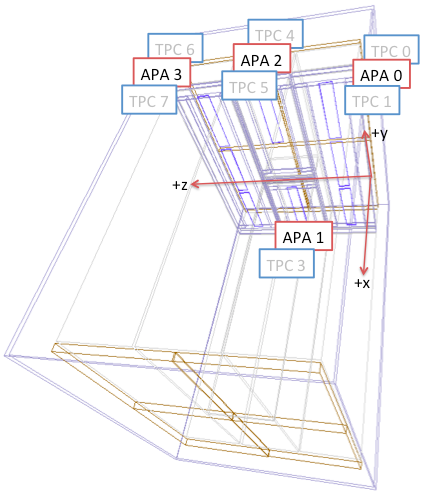
\includegraphics[width=8cm]{35tonGeometry.png}
  \caption[The 35~ton TPC geometry.]{The 35~ton TPC geometry and coordinate system \cite{35tonGeometryAlion2014}.  The blue frames represent the APAs and the orange the CPAs.  The eight separate drift volumes resulting from the modular TPC form are labelled TPC0--7.}
  \label{fig:35tonGeometry}
\end{figure}

The cathode and HV feedthroughs are designed to facilitate a voltage of 120~kV, providing the nominal field of 500~V/cm.  A field cage constructed using FR4 printed circuit board surrounds the open sides of the TPC to set up the necessary electric field.  This was the old LBNE design and has since evolved in the current DUNE outlook; it still enabled a study of the required field within a LArTPC however.

The TPC readout is similar to the DUNE design, with cold preamplifiers, signal shaping and digitisation implemented in ASICs mounted on front end boards at the ends of the APAs.  This is the first time a fully cold signal readout has been implemented in a LArTPC experiment and will be discussed in more detail in Section~\ref{sec:35tonElectronicsReadout}.

%----------------------------------------------------------------------------------------------------------------------------------------------------------------------------
\subsubsection{Photon Detectors}\label{sec:35tonPhotonDetectors}

Three design of photon detector were utilised in the 35~ton, none of which are current far detector considerations.  There were implemented within APAs in between the wire planes as eight separate units, demonstrated in Figure~\ref{fig:35tonPhotonDetectors} \cite{35tonPhotonDetectors}.

\begin{figure}
  \centering
  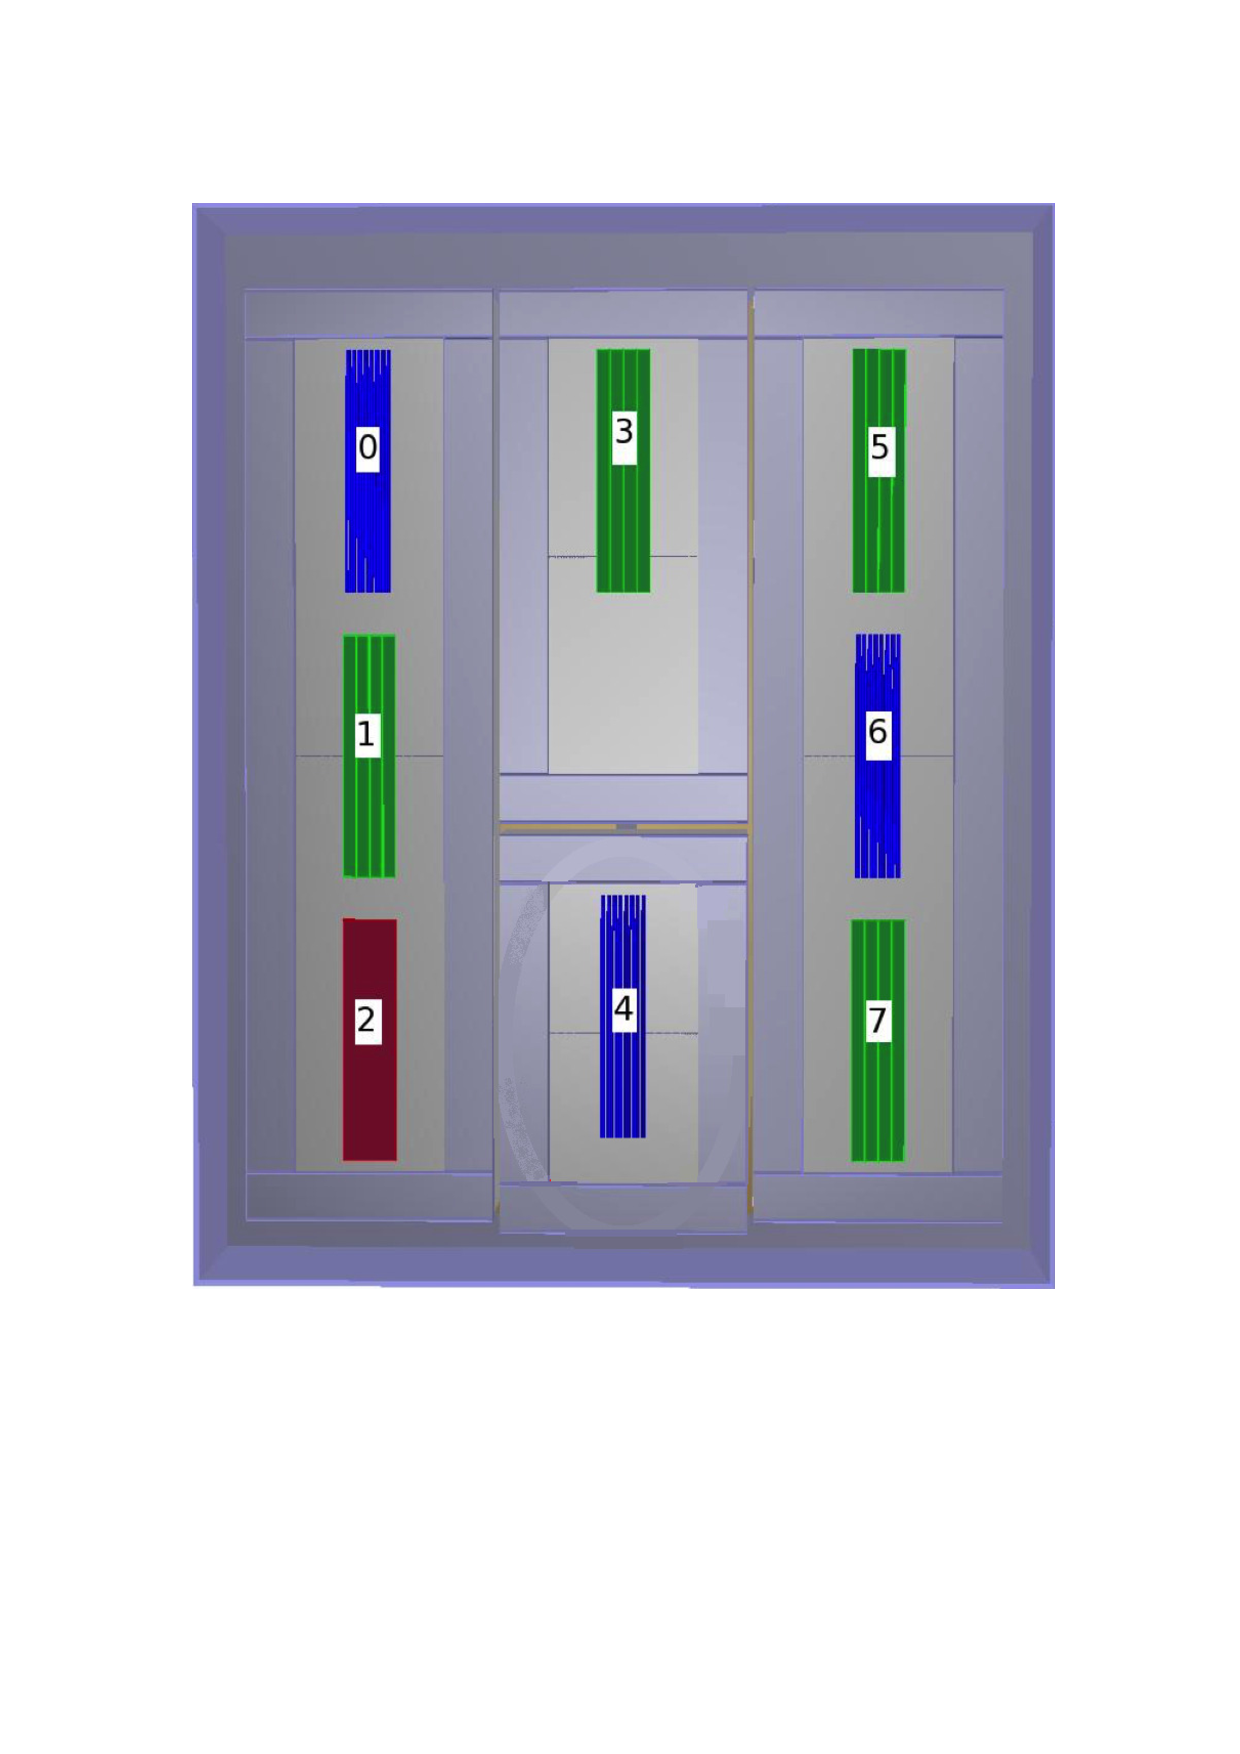
\includegraphics[width=6cm]{35tonPhotonDetectors.pdf}
  \caption[Photon detector units as implemented within the 35~ton APAs.]{Photon detector units as implemented within the 35~ton APAs \cite{35tonPhotonDetectors}.  The green detectors are the most similar to the current DUNE design and consist of a plastic bar with wavelength shifter (WLS); the blue and red detectors utilise designs of bundled fibres and plates embedded with WLS fibres respectively.}
  \label{fig:35tonPhotonDetectors}
\end{figure}

All detectors were read out by SiPMs which send analog signals outside the cryostat, via optical cables, for processing.  It was following experiences from the 35~ton that the current DUNE far detector design evolved (shown in Figure~\ref{fig:DUNEPhotonDetectors}).  In this plan, the detectors are orthogonal to the 35~ton versions and are inserted after the wire wrapping.

%----------------------------------------------------------------------------------------------------------------------------------------------------------------------------
\subsubsection{External Counters}\label{sec:35tonExternalCounters}

In order to provide an additional external trigger system, the 35~ton detector is instrumented with CRCs repurposed from the CDF muon upgrade detectors \cite{CDFCounters2005}.  Most are located on the outer walls of the cryostat, around all four sides and on top of Plate~B on the roof.  There are additional counters in the ceiling of the building directly above the 35~ton cryostat.  The positioning of all the scintillator paddles is shown in Figure~\ref{fig:35tonExternalCounters}.  There are two separate triggers provided by the counters: the `telescope trigger' caused by coincident hits recorded by the counters in the ceiling and those on the cryostat roof and the `horizontal trigger' caused by coincident counter hits on opposite walls of the cryostat (further subcategorised into `EW' and `NS' triggers).  The trigger rate for telescope muons is on the order of 60~Hz whilst horizontal muons trigger at a rate of around 2-3~Hz.

\begin{figure}
  \centering
  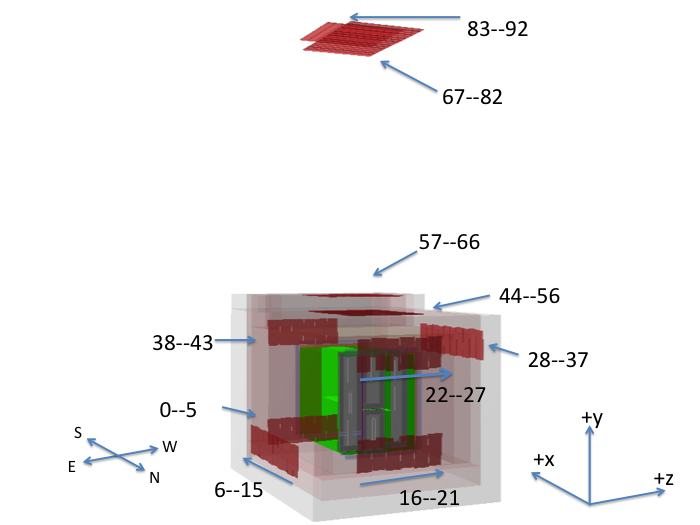
\includegraphics[width=12cm]{35tonExternalCounters.png}
  \caption[The location of the external counters positioned around the outer walls and in the ceiling above the 35~ton cryostat.]{The location of the external counters positioned around the outer walls and in the ceiling above the 35~ton cryostat \cite{35tonExternalCounters}.}
  \label{fig:35tonExternalCounters}
\end{figure}

%----------------------------------------------------------------------------------------------------------------------------------------------------------------------------
\subsection{Data Acquisition}\label{sec:35tonDataAcquisition}

The process of reading out the data from charge deposits on the anode planes through to the resulting data file on disk which may be utilised for subsequent analysis is the subject of this section.  The hardware components, including all readout electronics and processing units, will be briefly described in Section~\ref{sec:35tonElectronicsReadout}.  The data formats produced by the readout components are the subject of Section~\ref{sec:35tonDataFormats} before the software composing the data acquisition (DAQ) system is overviewed in Section~\ref{sec:35tonDAQ}.

%----------------------------------------------------------------------------------------------------------------------------------------------------------------------------
\subsubsection{Electronics and Readout}\label{sec:35tonElectronicsReadout}

The Front End Mother Boards (FEMBs) mounted on the end of the APAs contain two ASICs \cite{DeGeronimo2011,Thorn2012}; the `front end ASIC', which provides signal time-shaping at either 0.5~$\mu$s, 1.0~$\mu$s, 2.0~$\mu$s or 3.0~$\mu$s and amplification at gain settings of either 4.7~mV/fC, 7.8~mV/fC, 14~mV/fC or 25~mV/fC; and the `ADC ASIC' (Analog-Digital-Conversion) to perform 12-bit digitisation.  Different electronics response settings are demonstrated in Figure~\ref{fig:35tonFEASIC}; a configuration of 3~$\mu$s, 14~mV/fC was selected for normal data taking in order to maximise the signal/noise ratio in the collected data.  The digitised signals are extracted by Reconfigurable Computing Elements (RCEs) \cite{Herbst2014}, developed at SLAC, which trigger, buffer and format the data and send it downstream to the DAQ framework.  The digitising rate is 2~MHz, with the unit of time corresponding to an ADC sample described as a `tick' and equal to 500~ns.

\begin{figure}
  \centering
  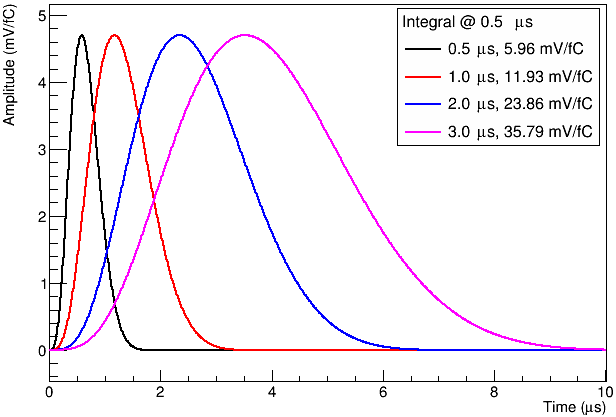
\includegraphics[width=10cm]{35tonFEASIC.png}
  \caption[Electronics response of the front end ASIC for different configuration settings.]{Electronics response of the front end ASIC for different configuration settings. {\color{red} Do I need this?}}
  \label{fig:35tonFEASIC}
\end{figure}

The photon detector information is digitised outside the cryostat by custom built units named `SiPM Signal Processors' (SSPs) \cite{SSPManual2016}, built at Argonne National Lab.  Each SSP reads out 12 channels and contains a fully differential voltage amplifier and a 14-bit ADC for signal digitisation.  Along with the RCE output, the SSPs transmit the processed signals to separate computers running the DAQ software.

The triggers are handled by the Penn Trigger Board (PTB), developed at the University of Pennsylvania, which also manages the CRC readout \cite{}.  A simplified block diagram of the triggering system is shown in Figure~\ref{fig:35tonTriggering}.  The PTB is designed to receive sub-system triggers (e.g. from the PDS) and generate global triggers along with timestamps, including internal triggers, for the whole detector.  It is additionally the front-end for the counter system and handles the reading out of all channels, forming counter `hits' (when a counter has turned on or off) and constructing triggers based on coincidences of these counter hits.  It has a backend which is designed to by compatible with the DAQ system and sends all information downstream to the acquisition software after the on-board logic has formed the relevant data products.

\begin{figure}
  \centering
  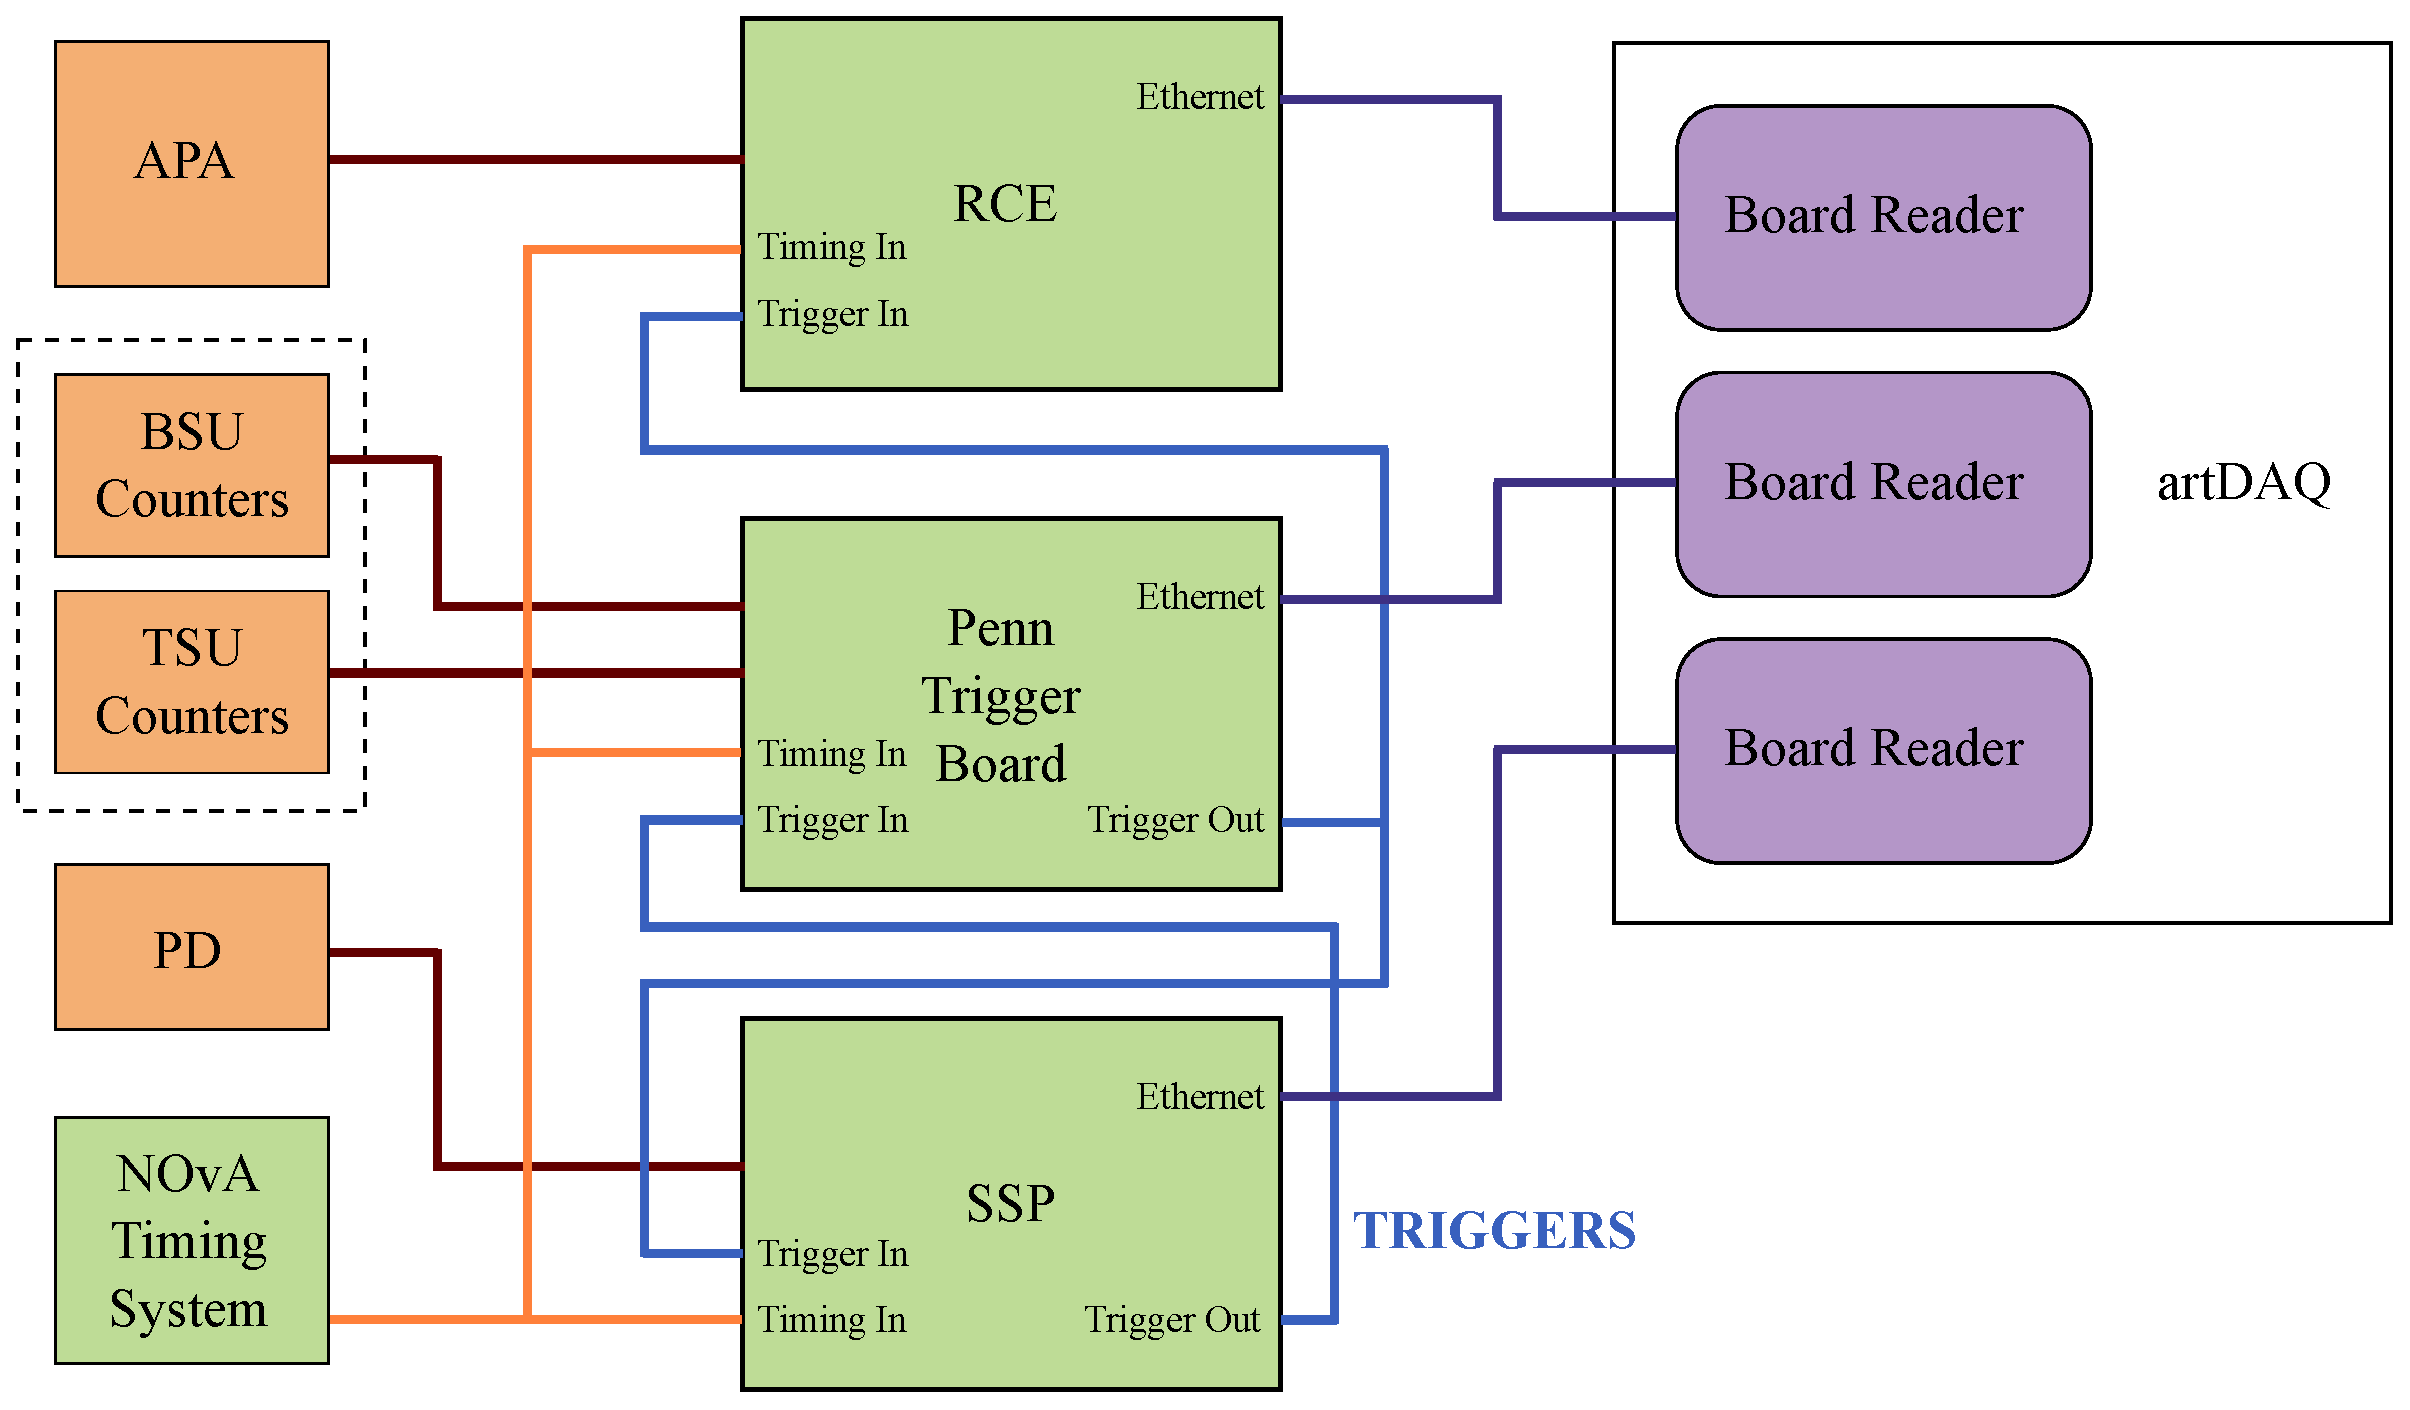
\includegraphics[width=12cm]{trigger_system.eps}
  \caption[Block diagram showing the triggering system for the 35~ton Phase~II.]{Block diagram showing the triggering system for the 35~ton Phase~II.  The Penn Trigger Board handles triggers from the CRCs and also from other detector components, such as the PDS.  Adapted from \cite{}.}
  \label{fig:35tonTriggering}
\end{figure}

%----------------------------------------------------------------------------------------------------------------------------------------------------------------------------
\subsubsection{35~ton Data Formats}\label{sec:35tonDataFormats}

The raw data format employs the concept of a `millislice' as a unified data structure common across all detector subcomponents.  An event is a collection of millislices, with one for each of the components being utilised (RCEs, SSPs, PTB).  Each contains substructure unique to the detector element; a simplified overview is provided in Figure~\ref{fig:35tonDataFormat}.

\begin{figure}
  \centering
  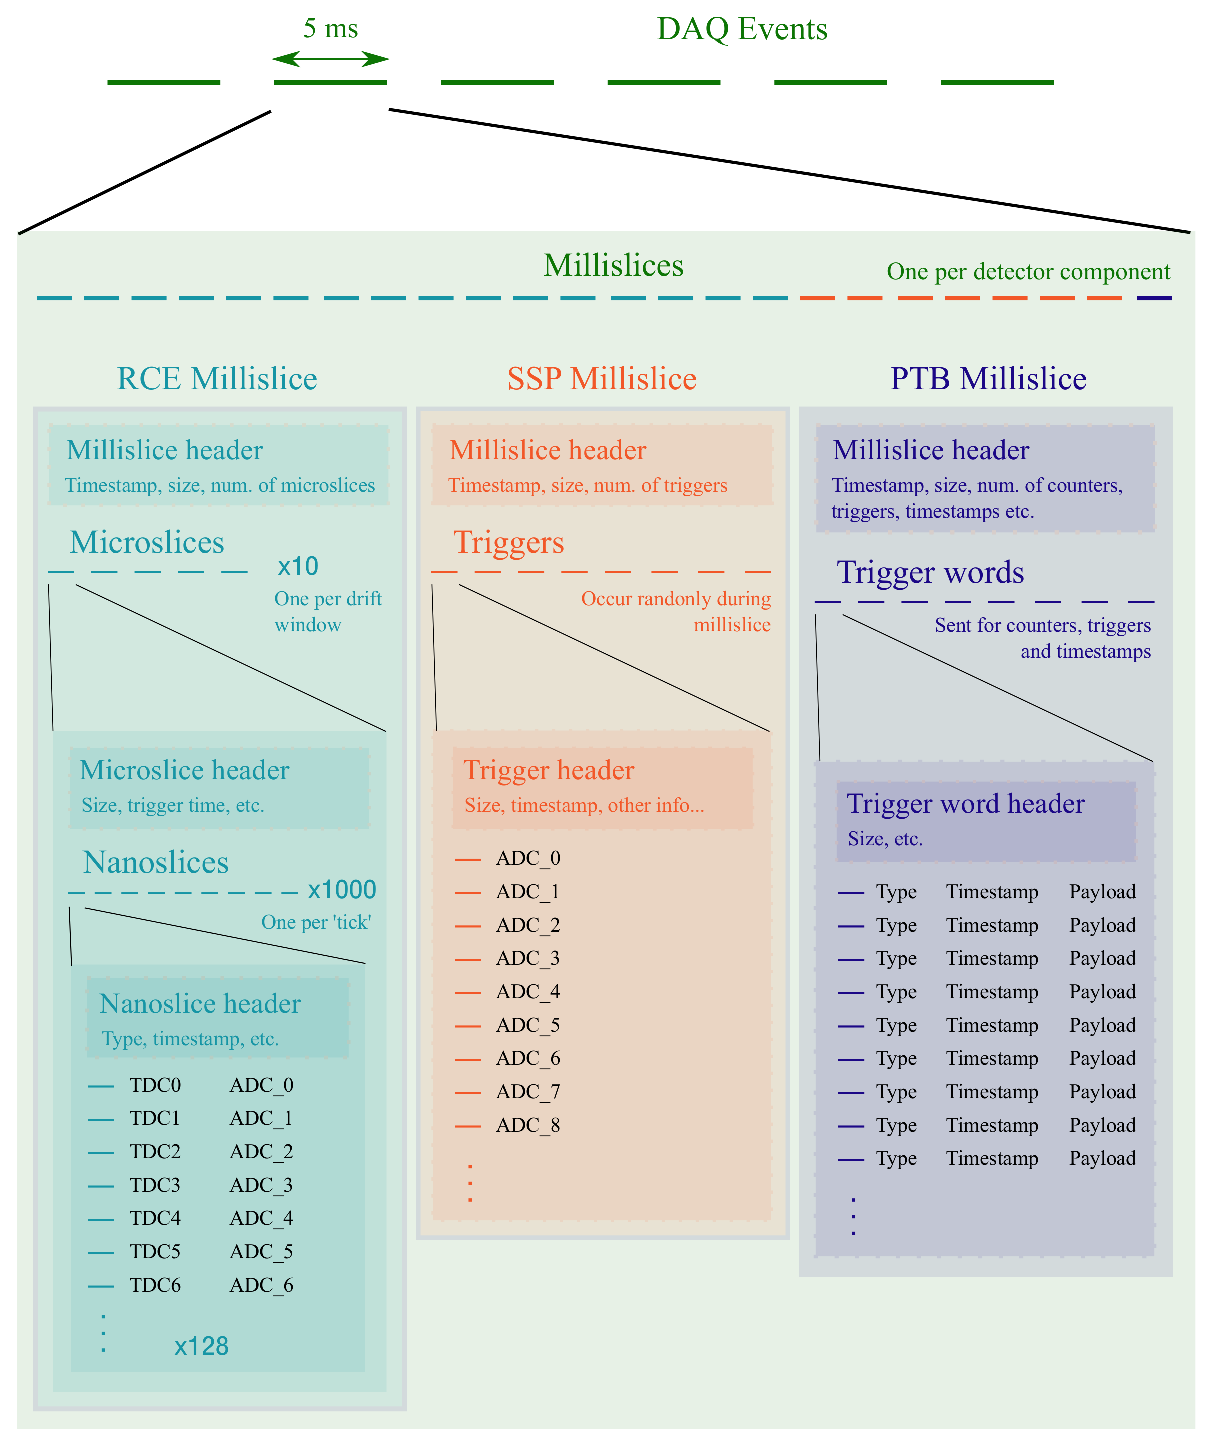
\includegraphics[width=14cm]{data_format.eps}
  \caption[35~ton data format]{Demonstration of the format used in 35~ton raw data.  A `DAQ event' is composed of a single millislice from each component, each containing further substructure unique to the readout elements.}
  \label{fig:35tonDataFormat}
\end{figure}

The raw format for the TPC data is complicated and has many levels of structure.  The 2048 TPC channels are read out out by 16 FEMBs, each processed by an RCE and represented by a separate millislice.  For the TPC data, a millislice contains all the information for 128 channels.  This data also has further substructure; a millislice is composed of N `microslices', with each microslice containing M `nanoslices'.  A nanoslice contains 128 ADC values, representing one tick worth of data for 1/16th of the detector.  A microslice thus contains this information for a `drift window' (N ticks) and a millislice a collection of M drift windows.  For the normal data running, N was set to 20 and M was 1000.

The data structure output from the SSPs and the PTB is a millislice consisting of a series of triggers filled with relevant information when required.  In the case of the photon detectors, an `SSP trigger' simply describes the waveform for a given channel as a list of ADC values, one for each tick.  A `PTB trigger' is either a counter hit, a trigger or a timestamp and contains a `trigger word' with the type, the timestamp and a variable payload describing relevant further information, such as the channel number or trigger type.  The triggers are created and saved in the SSP and PTB millislices regularly when self-triggered, or during an external trigger event provided by the PDS or the CRCs and handled by the PTB as demonstrated in Figure~\ref{fig:35tonTriggering}.

As data is collected, the RCEs continuously create and save microslices to send to the DAQ to form a millislice.  These microslices are empty (contain no nanoslices) until a trigger is received, at which point nanoslices are made and saved within each microslice.  Additionally, a buffer is in place to save a certain number of full microslices (containing nanoslices) before the microslice containing the trigger.  A certain number of full microslices proceeding the trigger are also recorded by the RCEs.  During normal running, a `$5+1+9$' format was employed; five microslices containing nanoslices before the trigger was received, the microslice containing the trigger, and the nine following microslices.  It should be further noted that, since the DAQ was designed for continuous data readout, these microslices need not necessarily be within the same millislice: it is possible for the trigger to occur in, for example, Microslice~18 of a certain millislice, resulting in the 15 filled microslices straddling successive millislices.  This is demonstrated in Figure~\ref{fig:35tonTriggeredEvent} and results in real `physics events' being saved in separate `DAQ events'.  To account for this, a splitter/stitcher module has been designed to extract the actual triggered events from the raw data and repackage them into a useful event structure.  This is the first stage before all offline analysis with the 35~ton data.

\begin{figure}
  \centering
  \includegraphics[width=16cm]{triggered_event.eps}
  \caption[Demonstration of how TPC data from a triggered event in a LArTPC is saved when employing a DAQ with continuous readout]{Demonstration of how TPC data is saved when using a DAQ designed for continuous readout.  The black arrows represent hypothetical triggers occurring within the duration of a particular millislice.  In each case, the five preceding microslices and the nine proceeding microslices are filled with nanoslices and saved; all other microslices are saved with no nanoslices since they contain no useful data.  An example of such an event is shown occurring in Millislice~0 in the figure.  As described in the text, a trigger can cause the useful microslices to straddle consecutive millislices; this is represented in the following millislices in the figure.}
  \label{fig:35tonTriggeredEvent}
\end{figure}

%----------------------------------------------------------------------------------------------------------------------------------------------------------------------------
\subsubsection{35~ton DAQ}\label{sec:35tonDAQ}

Experiments at FNAL are migrating to \textit{artdaq} \cite{Biery2013}, a centrally-maintained data acquisition system built on the art framework utilised by all offline software written for experiments hosted at the lab.  The DUNE 35~ton experiment was one of the first to use this new software (only LArIAT had previously used it for data taking) and used an experiment specific system named \textit{lbne-artdaq}.  A general overview of lbne-artdaq is shown in Figure~\ref{fig:lbne-artdaq}.

\begin{figure}
\centering
  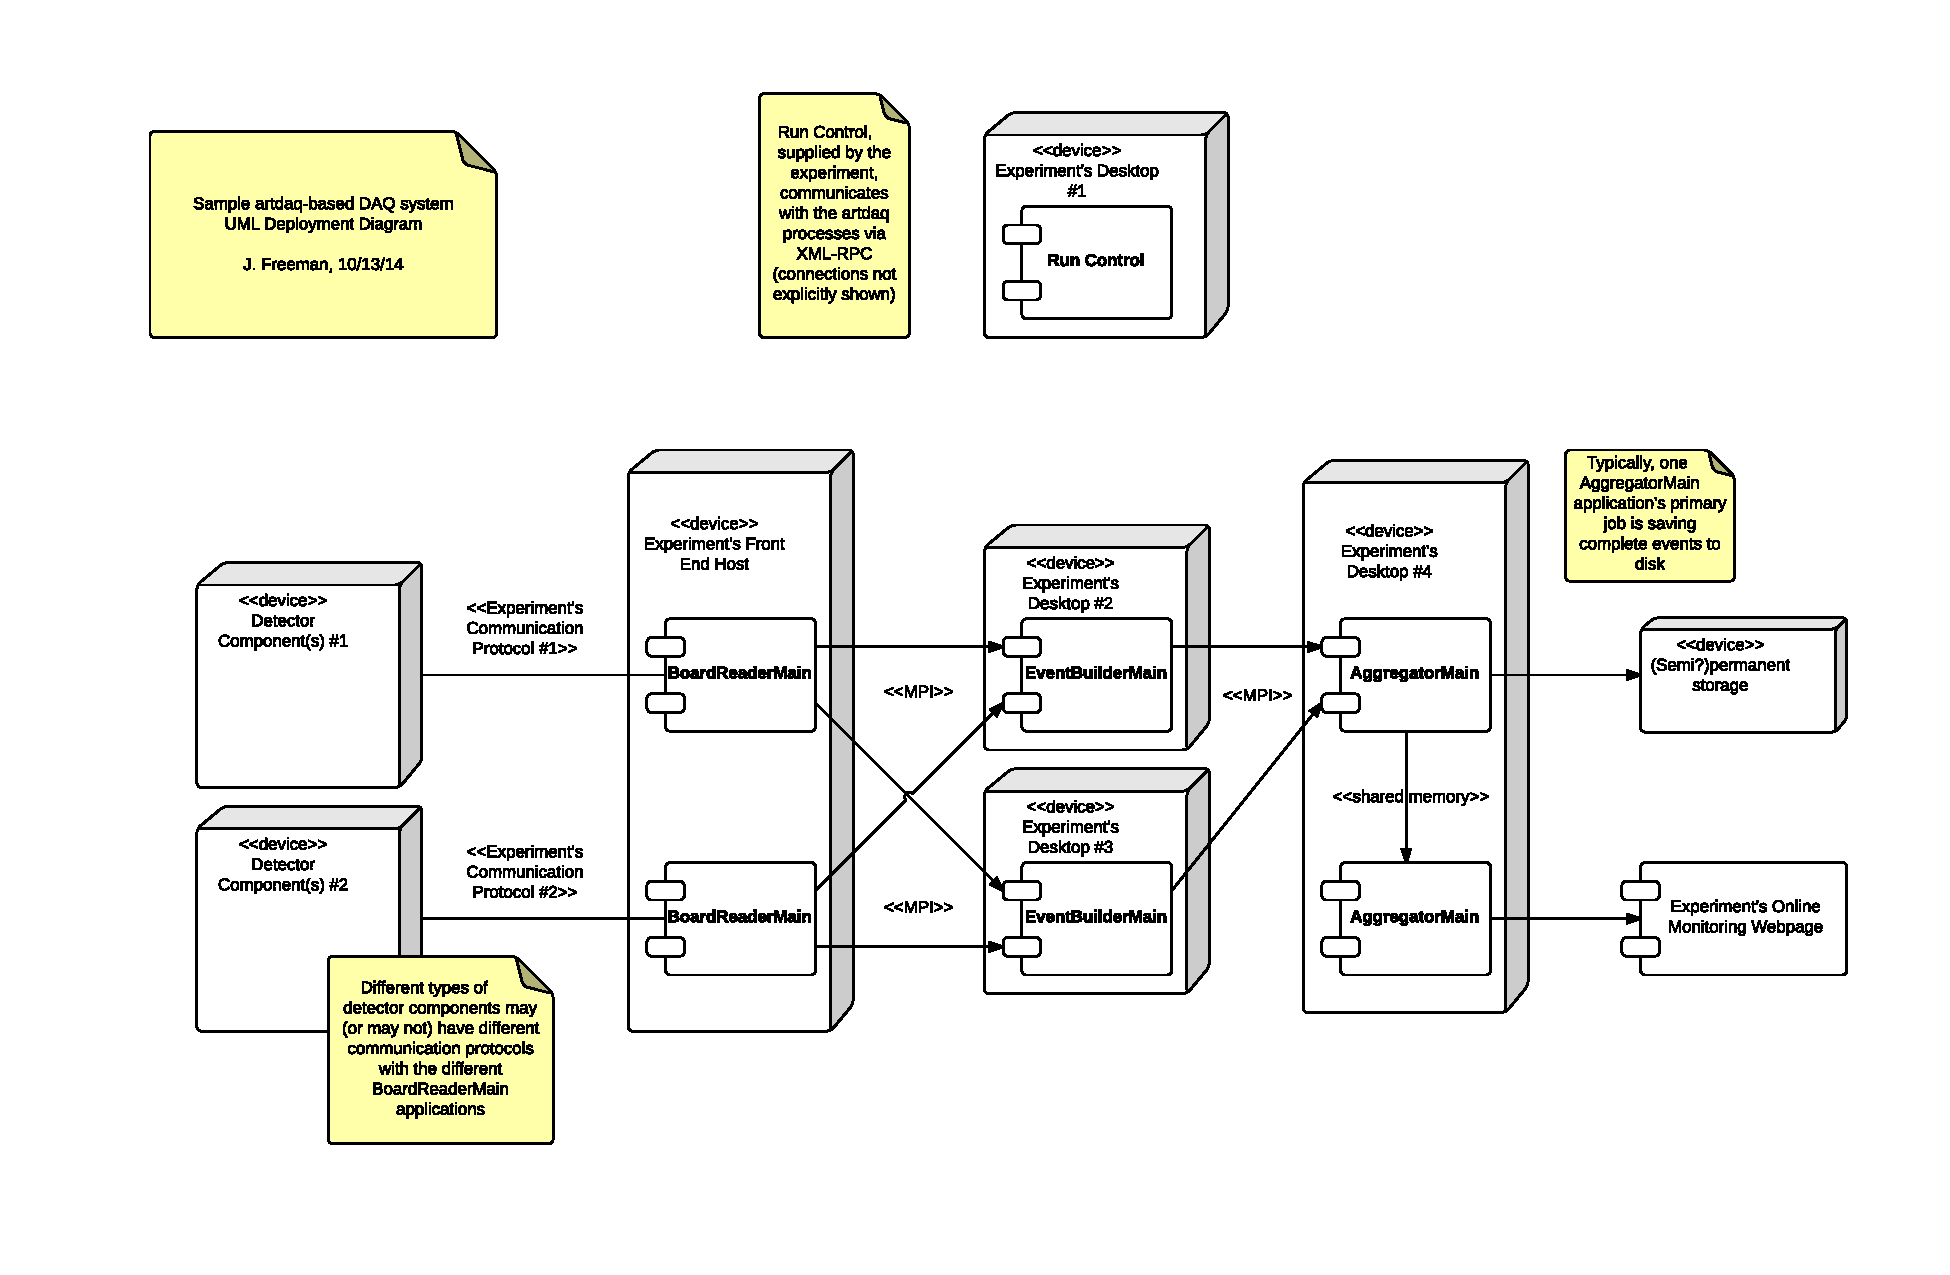
\includegraphics[width=16cm]{artdaqFramework.pdf}
  \caption[The \textit{lbne-artdaq} framework]{Overview of the \textit{lbne-artdaq} framework used for data acquisition by the DUNE 35~ton experiment \cite{Freeman2014}.}
  \label{fig:lbne-artdaq}
\end{figure}

Data flows from left to right and pass through components common to most DAQ systems.  Closest to the detector components (i.e. the RCEs, SSPs and PTB) are the board readers which take the output from the firmware and send it downstream to the event builders.  There exists a board reader for each of the detector components (totalling 24), with each is unaware of the existence of the others.  It is the job of the event builders to assemble a full `event' from these individual `fragments' passed on from each of the detector elements.  An event is complete once composed of a full set of fragments and the event builders will wait to receive them all before sending the data onwards to the aggregators.

There are two aggregators which take the full events but process them in very different ways.  All the data passes through only the first aggregator, whose function it is to write the output to disk and thus end processing by the DAQ.  The second aggregator receives no events but instead has access to the shared memory occupied by the data as it passes through the first aggregator; it is thus designed specifically for the purpose of monitoring and in no way affects the data or the output from the first aggregator.  This will be discussed futher in Chapter~\ref{chap:OnlineMonitoring}.

The 35~ton DAQ was designed to be `triggerless', with the ability to perform continuous readout.  This is an important feature of the far detector DAQ which is required to ensure data may be recorded safely for non-neutrino beam events, such as nucleon decay or a supernova burst.  This requires high levels of suppression to ensure rapid movement of data through the system.  In particular, zero suppression for the TPC has been designed such that only ADC values around a window of interest will be kept, vastly reducing the amount of data for the framework to handle.  The DAQ was additionally designed to run is various `modes', such as `scope mode', which focusses on a single channel during running, and `burst mode', designed to collect a sample of data from all channels for a given time upon receiving a trigger.

%----------------------------------------------------------------------------------------------------------------------------------------------------------------------------
\subsection{The Sheffield Camera System}\label{sec:SheffieldCameras}

There are many motivations for developing a camera system which operates at cryogenic temperatures as interest in experiments utilising LAr and LXe (as many dark matter experiments, such as Lux-Zeplin \cite{LZCDR2015}, are considering) progresses.  These include visual monitoring of the cryostat after sealing, including observing the cooldown and filling with cryogenic liquids, and to monitor HV discharge problems.  This latter issue has become cause for concern as LArTPC experiments with very large voltages are being developed; for example, DUNE will require a cathode HV of $-190$~kV.  Understanding the dielectric properties of LAr is therefore of paramount importance, with recent research suggesting breakdowns occurring at only 40~kV/cm \cite{Blatter2014}.  An additional aim of the 35~ton Phase~II experiment was to study the effects of HV and to search for evidence of HV breakdown of the LAr which may be used to influence the design of future LArTPC experiments in order to mitigate against these effects.  This is the primary motivation of the camera system deployed in the 35~ton cryostat \cite{35tonCameras2017}, designed at the University of Sheffield and described in this section.

The 35~ton was instrumented with eight cameras; six to monitor high-field locations within the cryostat and for detecting visual sparks from HV breakdowns, and two for diagnosis of different cryogenic systems including the cooldown sprayer and the phase separator.  The fields of view of each of the cameras are demonstrated in the calibration images shown in Figure~\ref{fig:35tonCamerasImages}.

\begin{figure}
  \centering
  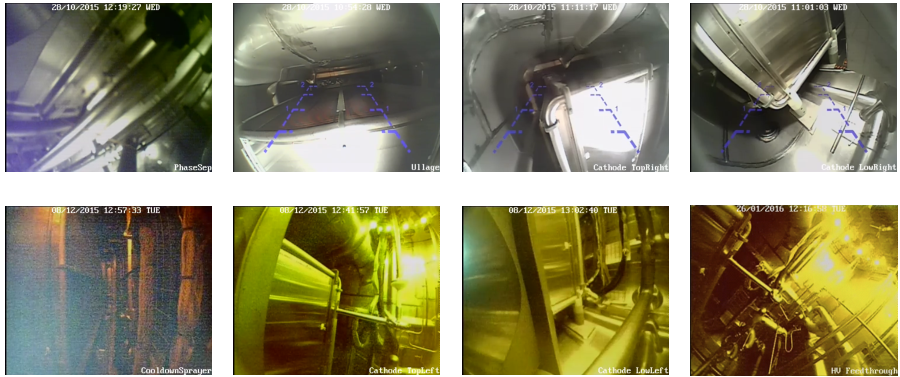
\includegraphics[width=15cm]{35tonCamerasImages.pdf}
  \caption{The calibration images for the 8 cameras in the system.  Upper (left to right): phase separator, ullage, cathode top right, cathode bottom right.  Lower (left to right) cooldown sprayers, cathode top left, cathode bottom left and high voltage feedthrough.  The upper images were taken with a halogen light illuminating the cryostat, prior to it being sealed up.  The lower images were taken with the LED ring light on, with the cryostat sealed up. All images are left-right inverted due to software.  Taken from \cite{35tonCameras2017}.}
  \label{fig:35tonCamerasImages}
\end{figure}

%----------------------------------------------------------------------------------------------------------------------------------------------------------------------------
\subsubsection{The Camera System}\label{sec:35tonCameraSystem}

Previous cameras designed to study cryogenic liquids have either been placed outside the volume or been maintained in a heated vessel for protection from the cold surroundings.  A system which operates directly in cryogenic temperatures is desirable when applying the technology to larger-scale cryostats and for possible use in the detection of secondary scintillation light.  Achieving this without an actively heated region in the cryostat is also advantageous to avoid boiling and disturbing the LAr in close proximity.  The camera system developed utilised Complementary Metal-Oxide Semiconductor (CMOS) cameras contained within a module alongside a temperature sensor and small resistive heater.  This is demostrated in Figure~\ref{fig:35tonCamera}.

\begin{figure}
  \centering
  \begin{subfigure}[t]{0.48\linewidth}
    \centering
    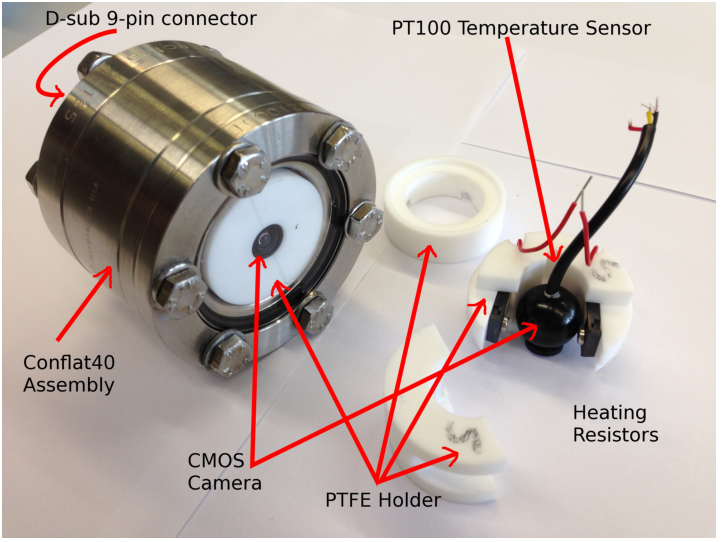
\includegraphics[width=0.98\textwidth]{35tonCameraPhoto.pdf}
    \caption{Photograph.}
    \label{fig:35tonCameraPhoto}
  \end{subfigure}
  \hfill
  \begin{subfigure}[t]{0.48\linewidth}
    \centering
    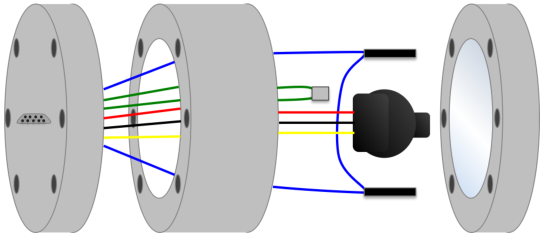
\includegraphics[width=0.98\textwidth]{35tonCameraSchematic.pdf}
    \caption{Schematic.}
    \label{fig:35tonCameraSchematic}
  \end{subfigure}
  \caption[An example camera module developed for the 35~ton Sheffield camera system.]{An example camera module developed for the 35~ton Sheffield camera system, taken from \cite{35tonCameras2017}.  Figure~\ref{fig:35tonCameraPhoto} shows a sealed camera module and the components of such a module.  Figure~\ref{fig:35tonCameraSchematic} demonstrates schematically the composition of a camera module: from left to right a CF40 flange with 9-pin D-sub feedthrough, double sided CF40 flange, PT100 sensor (green wires), camera (red, black and yellow wires), two heating resistors (blue wires) on either side of the camera connected in series, optical viewport on CF40 flange.}
  \label{fig:35tonCamera}
\end{figure}

The cameras are commerically sold as car-reversing cameras and are rated by the manufacturer down to $-40^{\circ}$C (233~K).  A wide range of cameras were tested and those which consistently performed well in tests whilst at cryogenic temperatures (submerged in liquid nitrogen) were selected.  Around half of these were found to reliably endure power cycling when cold (the inconsistency arising from operating the cameras outside of the recommendations) and it was these which were included in the modules used in the 35~ton.  The heating elements were included as a failsafe mechanism in case the cameras developed a requirement of warmer local temperatures to turn on after sustained periods in the cold.

Each camera contains 712~$\times$~486~pixels and has a roller shutter rate of 50~frames per second.  Their resolution at 10~mm was found to be $(2.0\pm0.5)$~mm at room temperature and $(1.5\pm0.5)$~mm at 77~K, with the improvement at lower temperatures due to a higher refractive index of LN$_2$ resulting in the light becoming less diffuse.  The minimum measurable light pulse, in both the warm and the cold, was observed to be 20~ns.  One notable change when operating the cameras at cryogenic temperatures was the chrominance output of the video signal.  The usual colour signal is observed as monochromatic when in the cold, possibly due to partial failures on the on-board encoding electronics.

Before installation, the response of the cameras to sparks was characterised by applying a HV across a printed circuit board (PCB) in LAr until breakdown was observed.  The discharge was between 40 and 60~ms and the cameras showed localised sparks persisting over multiple frames of exposure.  The trigger system, which relies on a percentage change in the number of different pixels between successive frames, was also able to successfully detect and automatically record on occurence of the sparks.

%----------------------------------------------------------------------------------------------------------------------------------------------------------------------------
\subsubsection{Operation and Outcomes of 35~ton Camera System}\label{sec:35tonCameraSystemOperation}

The camera modules were mounted on the existing piping from the cryogenic system within the 35~ton.  An example is shown in the photograph in Figure~\ref{fig:35tonCameraMounted}.  Data acquisition, operation and control was performed using a rack-based system containing a power supply, a temperature sensor reader, DAQ and computer control system.  Full details of the entire arrangement and all the interconnects are available in Figure~\ref{fig:35tonCameraDiagram}.

\begin{figure}
  \centering
  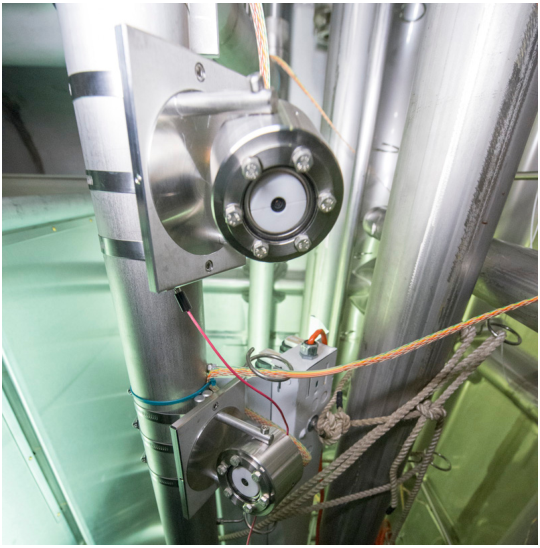
\includegraphics[width=8cm]{35tonCameraMounted.pdf}
  \caption[Two camera modules mounted on cryo piping in the 35~ton cryostat.]{Two camera modules mounted on cryo piping in the 35~ton cryostat.  Taken from \cite{35tonCameras2017}.}
  \label{fig:35tonCameraMounted}
\end{figure}

\begin{figure}
  \centering
  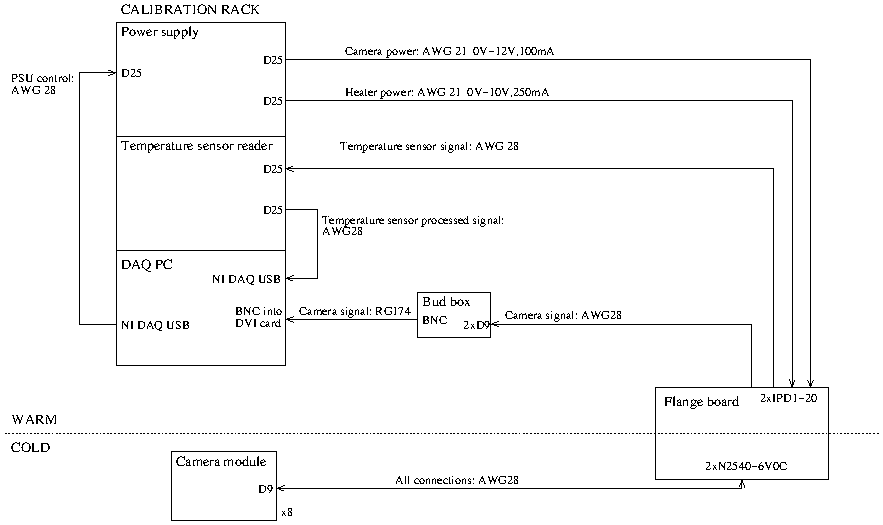
\includegraphics[width=12cm]{35tonCameraDiagram.pdf}
  \caption[Full system block diagram for the camera modules in the DUNE 35~ton prototype.]{Full system block diagram for the camera modules in the DUNE 35~ton prototype.  Taken from \cite{35tonCameras2017}.}
  \label{fig:35tonCameraDiagram}
\end{figure}

The cameras were characterised in room temperature following installation and the software trigger tested on the Xe flash light from the purity monitors (described in Section~\ref{sec:PurityMonitoring}).  The system ran continuously throughout the 10~weeks of the 35~ton Phase~II cooldown.  It was heavily utilised during cooldown and filling to monitor the inside of the cryostat and observe the rising liquid level (an excellent video of the LAr when level with one camera module is available at Reference~\cite{35tonCameraVideo}).  The entire system was power cycled successfully three times during TPC debugging and following the FNAL site wide power outage on 4rd March 2016.  The downtime ranged from 30~minutes to 9~days, with the cameras turned on without assistance each time.

The picture quality was observed to degrade noticeably over time, demonstrated in Figure~\ref{fig:35tonCamerasDegredation}, with significant variation between different camera modules.  When in darkness, a greater number of saturated or noisy pixels is observed across the cameras and when illuminated by the LED ring, the noise increase is noticable with a decreased colour depth.  This is likely due to signal transmission length, power cycling and increased prologure in the cold.

\begin{figure}
  \centering
  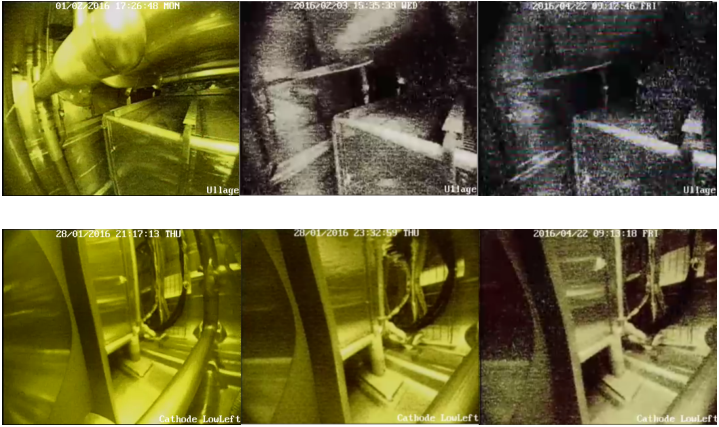
\includegraphics[width=12cm]{35tonCamerasDegredation.pdf}
  \caption[The variation in picture quality degradation in the 35~ton camera system is illustrated by the changes in Camera~1 and Camera~4 over time.]{The variation in picture quality degradation is illustrated by the changes in Camera~1 (upper) and Camera~4 (lower) over time. Left: prior to cooldown, centre: immediately post-cooldown, right: after 10 weeks submerged in LAr.  The field of view changes due to the change in refractive index.  Note that these are full colour images with no post-processing.  Taken from \cite{35tonCameras2017}.}
  \label{fig:35tonCamerasDegredation}
\end{figure}

Two suspected HV breakdowns occurred during normal operations at 60~kV but the system was unoperational as a result of the power outage during both.  Following the end of running, when testing the HV at 135~kV, four breakdowns occurred with three detected and triggered on by the camera system.  However, the location of the spark could not be determined clearly from the recorded video. This could be due to either the spark occurring outside the cryostat or the field of view of the cameras, an insufficient intensity or duration of the flash or the degredation in picture quality being such that the efficiency and sensitivity of the triggering system were compromised.

The camera system was shown to be successful and a hugely useful aid in 35~ton operations.  Despite not showing HV breakdowns clearly, the modules remained operational during the 35~ton Phase~II run and were valuable for monitoring purposes.  They were shown to trigger successfully on a test bench so it seems reasonable to conclude their inability to do so within the LArTPC was solely due to the degredation in picture quality, which must be improved if such a system were to be used in future LAr experiments.

%----------------------------------------------------------------------------------------------------------------------------------------------------------------------------
\subsection{Phase~II Run}\label{sec:35tonPhaseIIRun}

Following a long period of testing the detector components at FNAL, installation of the TPC and field cage was carried out in October 2015.  This was followed by the final parts of the system, such as the long drift region cathode, the purity monitors, HV feedthrough and cameras, in November 2015.  Following the Fermilab readiness clearance, operations began in December 2015.  This involved piston purging both LAPD and the 35~ton, filling LAPD with LAr delivered from the suppliers, cooling down the 35~ton cryostat and finally transferring the liquid argon from LAPD into the 35~ton.  This was completed by the end of January 2016.

{\color{red} NOTE: I've not added any plots at all from the cooling/filling/piston purge/purity etc etc from the filling stage; it's basically the same as Run I.  I can do if we think it'll be useful though (they are a bit nicer than the Run I ones!)}

The 35~ton Phase~II run officially started on 11th February 2016 upon the final liquid transfer into the cryostat and the starting of the pumps and recirculation of the LAr through the filtration system.  A week later, the HV on the cathode was ramped up to half nominal value: 60~kV, providing a drift field of 250~V/cm.  The intention was to ensure a sufficient amount of collected data was on disk before proceeding with increasing the HV up to the design voltage of 120~kV (500~V/cm) and even up to the maximum of 135~V/cm.

The start of the run was dedicated to many noise tests; it was immediately clear the noise on the TPC channels was much larger than anticipated even after the testing from the previous summer.  These tests involved studying each of the FEMBs separately and considering effects from other non-TPC detector elements by removing power from all systems in the cryostat before reintroducing components iteratively.  An additional `high noise state' was also identified which corresponded to a very high oscillatory noise level instaneously appearing on all channel simultaneously and remaining for up to hours at a time.  The noise problems in the 35~ton Phase~II will be discussed in more detail in Section~\ref{sec:35tonPhaseIIOutcomes}.

This time was also important as the stability of the DAQ was improved.  Near the beginning of data taking, it was uncommon for the DAQ to run for more than a few minutes with even a small subsection of components (RCEs, SSPs, PTB), with issues such as data throughput, disk writing speed and hardware interface issues contributing to a very unstable system.  In the months of installation and commissioning, the DAQ was the subject of much attention and progress on improving the framework progressed in parallel with the final installation, LAr filling and noise hunting.

Following the completion of the designated noise runs and the stabilising of the DAQ, the focus was on collecting as much data as possible before raising the HV, with the plan to run for at least week at 90~kV and 120~kV respectively.  However, the run was unfortunately cut short in the early hours of the morning of 19th March 2016 when a tube, part of the system which was introducing GAr from LAPD to the 35~ton purification network in order to maintain the LAr level, sheared and facilitated the introduction of air directly into the filters.  Within a few minutes, faster than it would have been possible to respond even if this incident had not occurred at 3~a.m., the filters were saturated and the entire volume of LAr in the 35~ton was poisoned.  The offending pipe break is shown in Figure~\ref{fig:35tonPipeBreak}.  This incident effectively concluded the data collection prematurely and meant the design HV could not be tested in good quality LAr and no data could be taken at nominal drift field.

\begin{figure}
  \centering
  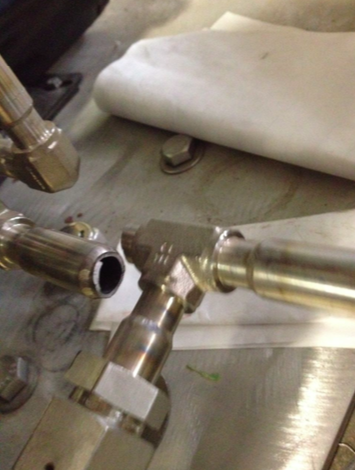
\includegraphics[width=6cm]{35tonPipeBreak.png}
  \caption[The broken pipe, originally part of the framework introducing gaseous argon from LAPD into the 35~ton to maintain LAr levels, which resulted in the poisoning of the whole LAr volume by allowing the introduction of air into the system.]{The broken pipe, originally part of the framework introducing gaseous argon from LAPD into the 35~ton to maintain LAr levels, which resulted in the poisoning of the whole LAr volume by allowing the introduction of air into the system.}
  \label{fig:35tonPipeBreak}
\end{figure}

The run is summarised in Figure~\ref{fig:35tonPhaseIIData}, showing the LAr purity as a function of time and notable incidents.  The bulk of collected data was either side of a site-wide FNAL power outage on 4th March 2016, after which it took a few days to recover the LAr purity.  After recuperating from this incident, an issue with the LN$_2$ values resulted in a cooling failure and the boiling off of a large portion of the LAr in the cryostat.  The pipe break occurred shortly after rectifying this issue.  The high frequency of these complications within such a short space of time motivated the description of this period of running as the `Bad News Period' on the figure.

\begin{figure}
  \centering
  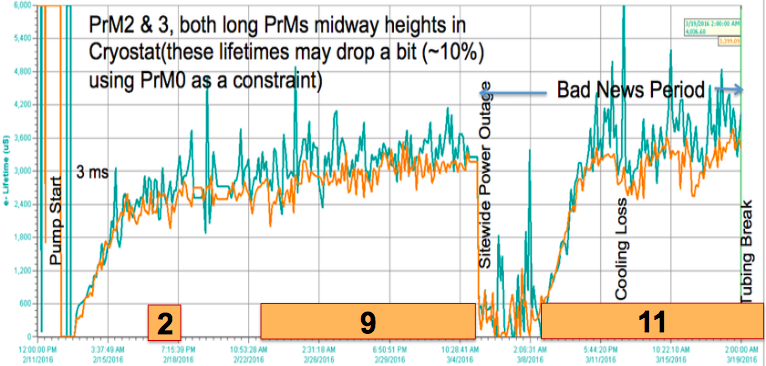
\includegraphics[width=15cm]{35tonPhaseIIData.png}
  \caption[The data taking period of the 35~ton Phase~II experiment.]{The data taking period of the 35~ton Phase~II experiment.  The electron lifetime measured by the two long PrMs in the cryostat is shown as a function of time, with the horizontal axis covering the period 11th~February -- 19th~March~2016.  The numbers within the orange boxes represent the amount of data taken with the drift field of 250~V/cm present, in days.  The major incidents which affected the LAr purity are shown on the figure.}
  \label{fig:35tonPhaseIIData}
\end{figure}

Most of the data taken were triggered using the horizontal muon trigger.  In the last week of running, the telescope trigger was deployed, with a large prescaling due to the high rate of cosmic muons, and the photon detectors were also used to trigger data taking.  Both systems appeared to work as intended but thorough testing proved impossible due to the temporal proximity to the unforseen termination of run.  Throughout data taking, the DAQ recorded data to disk at a rate of 1~Hz.  Because of the electronics noise and small signal/noise ratio, tests of data taking using zero suppression were unable to be performed.

Overall, the run provided 22 days of high quality (good LAr purity, high stable voltage, stable DAQ) data, albeit with much higher noise than anticipated.  An example electromagnetic shower observed in the data with strong signals in all planes is depicted in Figure~\ref{fig:FamousShower}.  The noise problems have resulted in limitations to the analyses possible with the 35~ton data and focus has shifted to studies utilising datasets unique to the 35~ton.  Some such analyses are the subject of Chapter~\ref{chap:35tonAnalysis}.

\begin{figure}
  \centering
  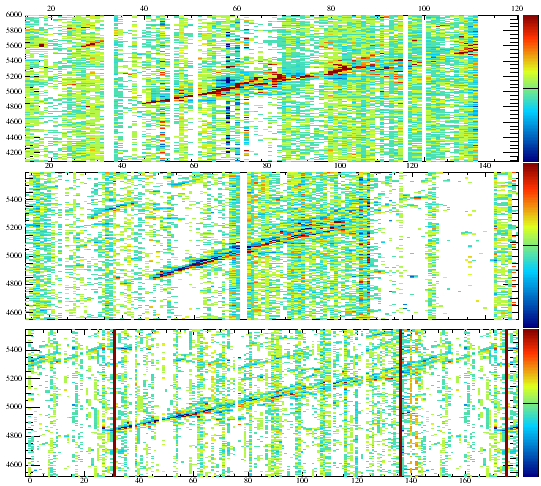
\includegraphics[width=12cm]{FamousShower.png}
  \caption[Event display depicting the charge deposited by an electromagnetic shower during the 35~ton Phase~II run.]{Event display depicting the charge deposited by an electromagnetic shower during the 35~ton Phase~II run.  The three views are, from the top down, the collection plane and the V and U induction planes.  Each shows the wire number on the horizontal axis and time, measured in units of tick ($\equiv$~500~ns) on the vertical axis.  Charge is represented by the colour scale on the $z$-axis.  The shower is clearly visible in all three planes and demonstrates the functionality of the 35~ton detector.}
  \label{fig:FamousShower}
\end{figure}

%----------------------------------------------------------------------------------------------------------------------------------------------------------------------------
\subsection{Outcomes of Phase~II}\label{sec:35tonPhaseIIOutcomes}

The 35~ton Phase~II collaboration successfully design, constructed, installed and ran a small-scale DUNE-style LArTPC and collected data whilst maintaining a good LAr purity, with electron lifetimes consistently reported above the DUNE requirement of 3~ms.  This is the first time a detector has been operated within a membrane cryostat and the integrated system has been strongly validated.  The complete process has been instructive and a great many lessons have been learned alongside the successes of the project.

This section will review all these outcomes and discuss how the experience will influence the DUNE program as it progresses towards the first far detector module.  In general, the experiment was a success with the majority of subsystems achieving or superceeding expectations.  Following the 35~ton Phase~II experience, there is no reason for reservation over ProtoDUNE as rapid development continues to be made.

%----------------------------------------------------------------------------------------------------------------------------------------------------------------------------
\subsubsection{Cryostat and TPC}\label{sec:35tonPhaseIIOutcomesCryostatTPC}

The cryostat and most TPC components behaved as expected and resulted in no unexpected functionality.  When filled with GAr, before the introduction of LAr, the cryostat was leak tested.  When this was performed in Phase~I a few issues were identified and had to be addressed; there were no complications during Phase~II commissioning however.  The pumps were not tested between phases and required a huge current to break them in with the cryostat already filled with LAr; this demonstrates how vital it is to assess all detector components before commissioning.  Other than the failing in the cooling system, all cryogenics performed excellently.  Since this incident occurred not long after the power outage, the alarm system had not been correctly brought back online, resulting in an avoidably large loss of LAr.  These are two of many examples of lessons learned from the 35~ton.

The HV and drift field presented no issues during the course of the run.  No confirmed breakdowns were observed at 60~kV but testing in clean LAr at 120~kV was not possible.  Although a voltage of 135~kV was attained and held for multiple days in contaiminated argon, the impurities are presumed to alter to dielectric properties of the material and therefore complete validation remains unproven.

Results from the purity monitors and temperature sensors suggest a stratification along the height of the LAr volume within the cryostat, similar to observations made during the Phase~I run.  The cause of this is likely due to returning LAr from the purification system being cooled below the `bulk temperature' by the phase separator and reentering near the bottom of the cryostat, resulting in reduced convection and poor mixing.  Resolutions, such as returning warmer LAr to the main volume, are being considered for future LArTPCs in an attempt to mitigate these effects and ensure a good, isotropic purity.

The TPC electronics were the largest source of shortfalls in the experiment and have significantly compromised the utility of the data.  During warm tests over summer 2015, it was evident the intrinsic noise levels in the ASIC electronics were higher than anticipated and an additional issue with the ADC ASIC was observed.  The digitisers are affected by bit-level corruption whereby the six least-significant bits (LSF) or most-significant bits (MSB) are erroneously reported as either 0x0 or 0x3F at a rate between 20\% and 80\% which is strongly dependent on the proximity of the true value to these `sticky' codes, and also on the temperature, the input current and the channel.  Along with this `stuck code' problem are futher issues with `stuck bits', where a particular bit is never set or cleared.  These issues may be somewhat mitigated in software but work is ongoing to rectify concerns before their use in ProtoDUNE.  The multiple problems with coherent and incoherent noise which characterise the 35~ton dataset are discussed further in Section~\ref{sec:35tonPhaseIIOutcomesNoise}.

%----------------------------------------------------------------------------------------------------------------------------------------------------------------------------
\subsubsection{Triggering Systems: Photon Detectors and Muon Counters}\label{sec:35tonPhaseIIOutcomesTriggeringSystems}

The photon detector system and external muon counters also achieved expectations.  Although the counters are unnecessary for the far detector, they proved critical to the success of the 35~ton.  The vast majority of data was recorded whilst triggering on throughgoing muons and, as will be discussed further in Chater~\ref{chap:35tonAnalysis}, all worthwhile analyses rely heavily on counter information.

The photon detection system (PDS) was shown to successfully record data in both externally triggered (when using the muon counters) and self-triggered modes, where the PDS sends a trigger to the PTB upon recieving a sufficient level of scintillation light.  The timing resolution of the detectors was shown to be better than 100~ns with respect to the counter timing, as shown in Figure~\ref{fig:35tonPhotonDetectorsResolution}, with signals as low as a single p.e. detected.  The attenuation length in LAr may be determined by considering the signal size of scintillation flashes, using counter trigger information to determine how far from the detectors the interaction occurred.  This is demonstrated in Figure~\ref{fig:35tonPhotonDetectorsAttenuation} and yields a measurement of $155\pm28$~cm.

Given the noise problems in the TPC data, it was not possible to do joint analyses using the photon detectors as planned.  The system performed well however and validated the concept of using WLS bars with SiPM readout as opposed to PMTs for the DUNE far detector design.

\begin{figure}

  \begin{minipage}[t]{0.48\linewidth}
    \centering
    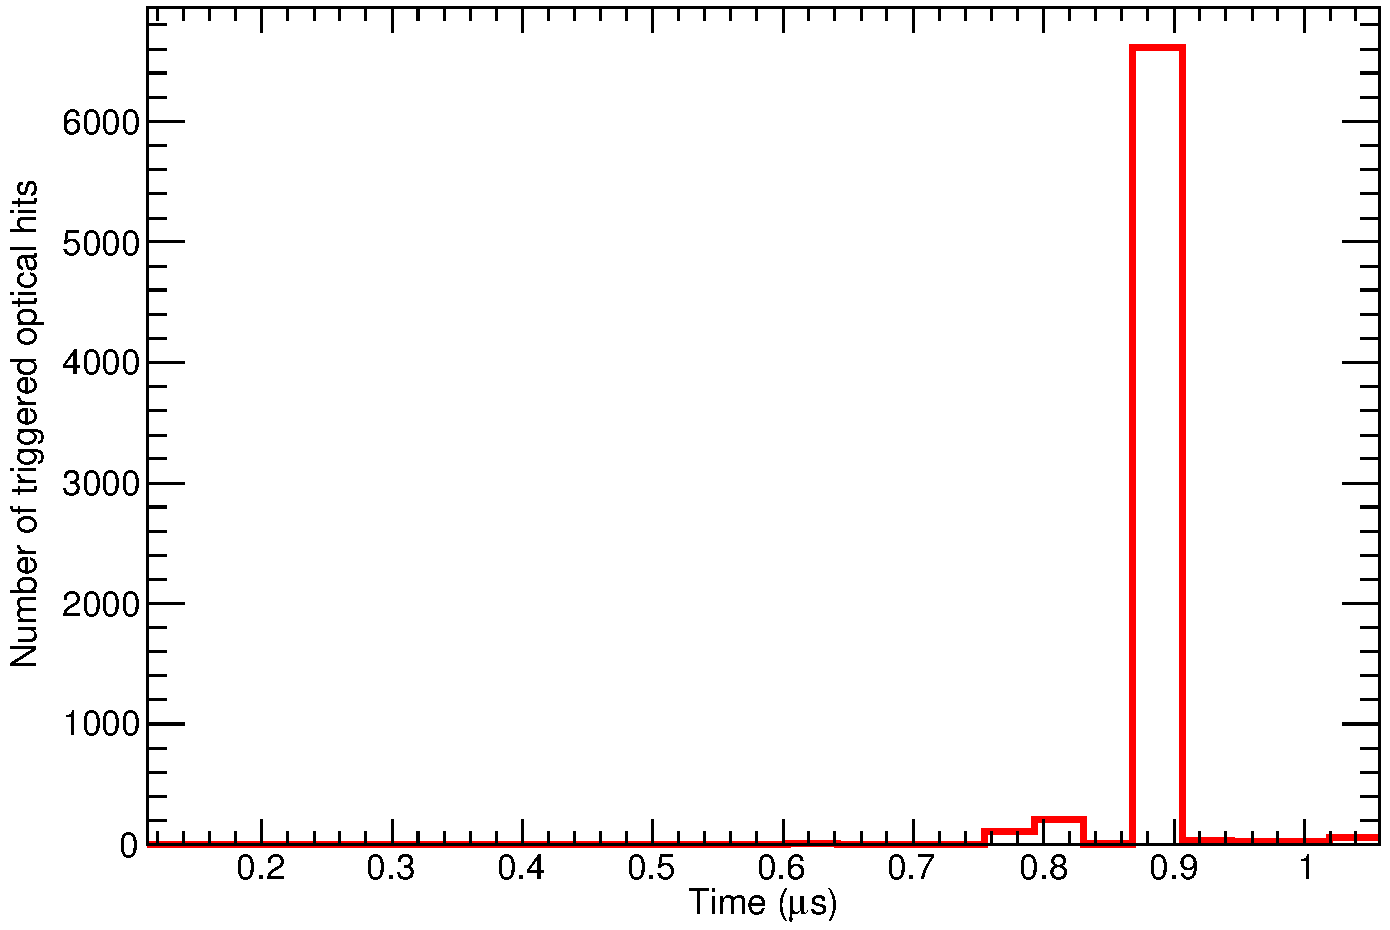
\includegraphics[width=0.9\textwidth]{35tonPhotonDetectorsResolution.pdf}
    \caption[Difference between optical hit peak times and muon counter trigger times for photon detector 3 in the 35~ton photon detection system.]{Difference between optical hit peak times and muon counter trigger times for photon detector 3 in the 35~ton photon detection system. The binning reflects the digitization time of the photon detector electronics.  Taken from \cite{35tonPhotonDetectors}.}
    \label{fig:35tonPhotonDetectorsResolution}
  \end{minipage}
  \hfill
  \begin{minipage}[t]{0.48\linewidth}
    \centering
    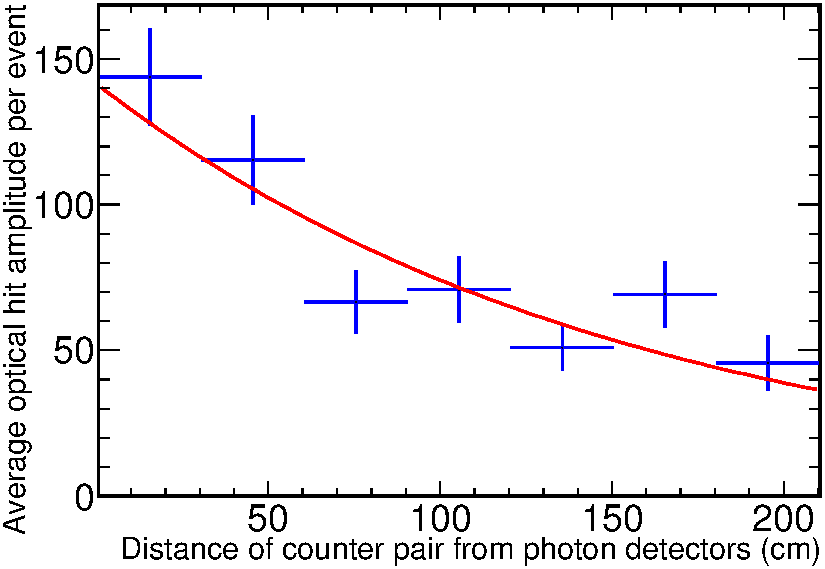
\includegraphics[width=0.9\textwidth]{35tonPhotonDetectorsAttenuation.pdf}
    \caption[Average Optical Hit Amplitude per Event vs. Counter Pair Positions for the 35~ton photon detection system.]{Average Optical Hit Amplitude per Event vs. Counter Pair Positions for the 35~ton photon detection system.  Error bars are statistical errors on mean hit amplitudes per bin.  Taken from \cite{35tonPhotonDetectors}.}
    \label{fig:35tonPhotonDetectorsAttenuation}
  \end{minipage}

\end{figure}

%----------------------------------------------------------------------------------------------------------------------------------------------------------------------------
\subsubsection{DAQ and Computing}\label{sec:35tonPhaseIIOutcomesDAQ}

The DAQ was remarkably consistent throughout data taking following the stabilisation period.  All components could be operated simultaneously with data written to disk at a steady rate, successfully demonstrating continous readout of the detector systems.  In total, $\sim$500k cosmics were recorded during the 35~ton Phase~II data taking, with an impressive capacity on disk of $\sim$30~TB.

It proved imperative to monitor the data during running as detector issues spontaneously arose on a regular basis.  The large volume of data was an additional issue and finding an optimum output file size, balancing number of data files on disk with size of each file and potential for data loss upon a DAQ crash, occupied a sizeable amount of commissioning time.  Additionally, a potentially disastrous failure in the alarm system for one of the computing racks resulting in serious overheating and the loss of all the machines which were running most of the online processes.

Data from the cold electronics were shown to be processed by the RCEs at a rate of 1~Gb/s but a bottle-neck in the framework restricted disk writing to 60~MB/s, resulting in an enforced reduced data flow through the system.  An event rate of 1~Hz was utilised during the run, much smaller than the design rate of 200~Hz.  This could have been improved by employing zero suppression in the TPC data but this was unable to be tested as planned in the 35~ton.  The event rate requires improvement before the far detector DAQ but work is underway and the experience with the 35~ton will be taken forward with most of the existing framework under development for use in ProtoDUNE.

%----------------------------------------------------------------------------------------------------------------------------------------------------------------------------
\subsubsection{Noise Issues}\label{sec:35tonPhaseIIOutcomesNoise}

An example muon track observed in the 35~ton data, along with typical waveforms recorded on the anode wires, is shown alongside an analogous muon track and detector response from simulation in Figure~\ref{fig:DataSimulationNoiseComparison}.  It is clear...

\begin{figure}
  \centering

  \begin{subfigure}[t]{\linewidth}
    \centering
    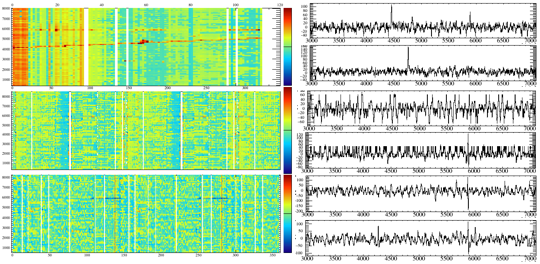
\includegraphics[width=\textwidth]{DataMuonCombined.png}
    \caption{}
    \label{fig:DataMuon}
  \end{subfigure}

  \begin{subfigure}[t]{\linewidth}
    \centering
    %\includegraphics[width=\textwidth]{SimulationMuonCombined.png}
    \caption{}
    \label{fig:SimulationMuon}
  \end{subfigure}

  \caption{}
  \label{fig:DataSimulationNoiseComparison}

\end{figure}

There were multiple sources of noise in the 35~ton detector with distinct `modes': the `normal noise state' (which still contains numerous issues) and the `high noise state' \cite{35tonNoise2016}.  The frequency bands of noise in each state is demonstrated in Figure~\ref{fig:NoiseStates}.

\begin{figure}
  \centering
  \begin{subfigure}[t]{0.48\linewidth}
    \centering
    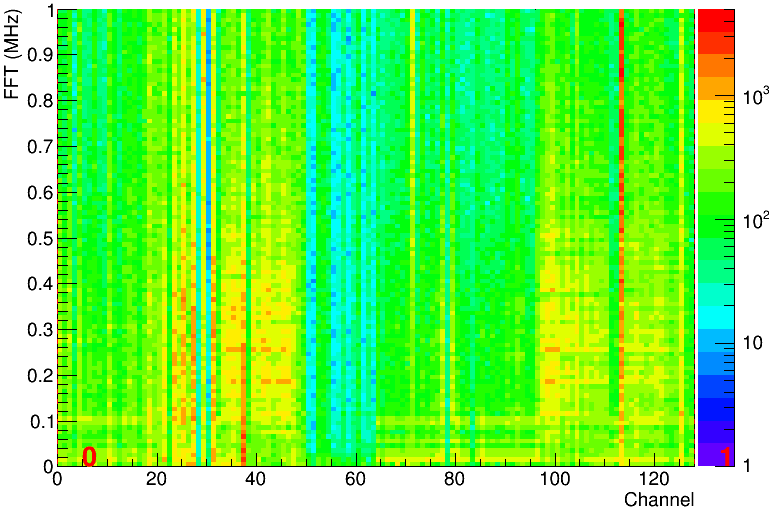
\includegraphics[width=0.98\textwidth]{FFTRun13079.png}
    \caption{Normal noise state, run 13079.}
    \label{fig:NormalNoiseState}
  \end{subfigure}
  \hfill
  \begin{subfigure}[t]{0.48\linewidth}
    \centering
    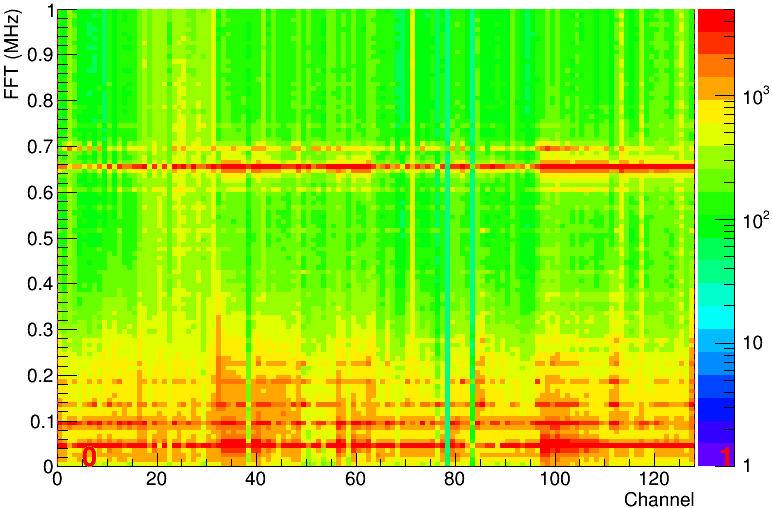
\includegraphics[width=0.98\textwidth]{FFTRun10286.png}
    \caption{High noise state, run 10286.}
    \label{fig:HighNoiseState}
  \end{subfigure}
  \caption[FFT of ADC values for RCE00 for two different noise states.]{FFT of ADC values for RCE00 for two different noise states.  During the normal noise state, the noise band at 11~kHz (faintly visible at 0.011~MHz in Figure~\ref{fig:NormalNoiseState}) is present across all channels in the detector and a lot of channels also see 100~kHz frequency noise.  The high noise state manifests across all channels in the detector as multiple frequency bands and render any collected data useless when present.}
  \label{fig:NoiseStates}
\end{figure}

The normal noise state is characterised by 11~kHz and 100~kHz bands.  The phase of the 11~kHz noise appears to alter every 64 channels, corresponding to the blocks of channels read out by ASICs sharing a common voltage regulator (four 16 channel ASICs).  The correlation between the waveforms observed on the channels maintained by the same regulator is evident in the plot shown Figure~\ref{fig:NoiseCorrelation}.  This was shown to be removed following the run by the addition of a 1~$\Omega$ resistor in series, effectively forming a low pass filter, and can be removed crudely in software using a coherent noise subtractor.  A similar phase shift in the 100~kHz noise is observed at the boundaries between FEMBs, which are each maintained separately by the low voltage power supply.  Again following the completion of the run, close inspection of the cabling found a short between the supply return line for the FE ASICs and the chassis ground for the supply.  Correcting this removed all noise sources and, along with the correlated component from the voltage regulators, explained all prominent noise frequencies in the normal mode.

\begin{figure}
  \centering
  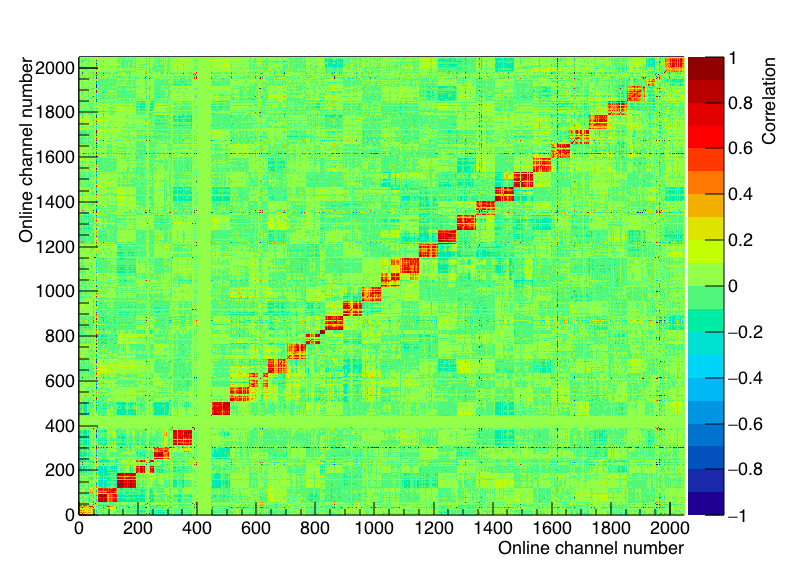
\includegraphics[width=12cm]{NoiseCorrelation.png}
  \caption{}
  \label{fig:NoiseCorrelation}
\end{figure}

The high noise state was entirely unanticipated but was characterised by several features: a very high noise level is observed without saturating the ASICs; multiple frequency bands, most under 300~kHz, are observed simultaneously across all channels in the detector; these frequency bands are consistent for the duration of the high noise state but change each time the state is entered; these frequencies are also observed on a spectrum analyser connected to an APA grid plane; the current draw of the ASICs is observed to drop when in the high noise state.  Furthermore, the high noise state was not observed when the cryostat was at room temperature and so could not be investigated subsequent to the end of the run.  It has been understood as a collective oscillation of all detector components which is spontaneously entered, roughly every few hours, during running.  Often, after a time period on the order of an hour, the system may egress from the state; it was also noted that power cycling the front end ASICs may also return the detector to the normal noise state.  The noise investigations after data taking were unable to definitively identify the conditions of the abnormality but have offered suggestions as to the likely causes.  The frequency of the oscillations, and the inability to induce the state in the warm system, argues stongly against external influences.  The source cannot be the anode wires as this would saturate the front end electronics and, given the necessary power required to sustain the oscillations on the grid plane, the only candidate is the low voltage power supply.  The difference between the 35~ton and MicroBooNE, which uses the same supplies has has not observed similar problems, is the length of cabling used in the 35~ton is around 10 times greater.  This may turn the negative feedback in a remote sense system into a positive feedback loop, causing the circuit to search for the correct voltage settings by overshooting and subsequently undershooting (i.e. oscillating) due to the round trip cable delay being longer than the circuit response time.  The strong frequency bands at 650~kHz, which are always present across all channels whenever the high noise state is entered, unlike the other frequencies, is likely due to the oscillating cable acting as a cable resonator.  During the run, it was observed that APA1 (the short, bottom centre, APA) was most prone to these issues and was actually left unpowered during much of the data taking.  This may be explained by considering the most likely coupling is to the FE electronics for this APA (the only one where these are at the bottom) to the grid plane, which then couples to the cathode on the short drift side and from there is transferred to the other APAs in the detector.  The decreased capacitance of the cable in air than when submerged in LAr explains why this state could not be induced following the end of operations.

Finally, it is observed that the minimum noise in the detector is higher than in MicroBooNE.  Although the induction wires are much longer, there is still an increase greater than could be accounted for by the larger capacitance of the wires.  The noise experts suggest there may be a common mode noise on the supply line which may intensify the overall noise levels without inducing the high noise state; this would enter via the cathode, then the grid planes and then the induction wires and would explain why this plane sees more noise than the collection view.

The noise issues encountered in the 35~ton, though unexpected, have been critical to understanding the issues which may be present in large scale LArTPCs and would be seriously detrimental to the DUNE project if encountered in the far detector.  Every effort has been made to understand the issues with the 35~ton and ensure the eventual success of the experiment.

%----------------------------------------------------------------------------------------------------------------------------------------------------------------------------
\section{Summary}\label{sec:35tonSummary}

The 35~ton experience, while unable to deliver the high quality data anticipated for the purpose of physics analyses, was invaluable to the DUNE strategy.  



















%% % The very first part of my thesis, written June 2015.  I'll leave it here to remember it!

%% %% \section{The DUNE 35ton LAr Prototype}

%% %% The DUNE far detector (see section
%% %% %\ref{sec:DUNEFD})
%% %% has a very large, complicated design including many features which are novel to this experiment. In order to optimise and minimise potential complications during construction an\
%% %% d commissioning, several levels of prototyping are necessary during the design. These include the membrane cryostat, a TPC within such a cryostat, full scale detector elements, \
%% %% installation test and complete vertical slice tests of all electronics. Many of these have been tested with the first of two DUNE prototypes, the 35-ton (ref Far Detector Extern\
%% %% al Review, May 19-20 2015).

%% %% There was a phase 1 run! \cite{LBNE35tonPhase1}

%% %% \subsection{Overview of the 35-ton}

%% %% The 35-ton is a

%% %% The 35~ton consists of a membrane cryostat (Section \ref{sec:35tonCryostat}), designed to be filled with 35 metric tons of liquid argon, and a small-scale DUNE-style detector (Section \ref{sec:35tonDetector}) including a TPC and photon detectors.  It was constructed in 2012 at PC4, a former proton facility in a decomissioned beamline, at Fermilab.  The Phase I run, without a detector, took place between December 2013 and February 2014.  Between February 2014 and September 2015 the detector was constructed and heavily tested at FNAL before being installed inside the cryostat ready for the Phase II run.  This took place between February 2016 and April 2016 (offically starting on 11th February, as I type!).

